
\documentclass[a4paper,DIV=12]{scrreprt}
\usepackage{listings}
\usepackage{underscore}
\usepackage[bookmarks=true]{hyperref}
\usepackage[utf8]{inputenc}
\usepackage[english]{babel}
\usepackage{graphicx}
\usepackage{multirow}
%\documentclass[12pt]{book}
\renewcommand*\familydefault{\sfdefault}
\usepackage{graphicx}
\graphicspath{{Imgs/}}
\usepackage{listings}
\usepackage{color}

\lstloadlanguages{C,C++,csh,Java}
\definecolor{red}{rgb}{0.6,0,0} 
\definecolor{blue}{rgb}{0,0,0.6}
\definecolor{green}{rgb}{0,0.8,0}
\definecolor{cyan}{rgb}{0.0,0.6,0.6}
\lstset{
language=csh,
basicstyle=\footnotesize\ttfamily,
numbers=left,
numberstyle=\tiny,
numbersep=0pt,
tabsize=1,
extendedchars=true,
breaklines=true,
frame=b,
stringstyle=\color{blue}\ttfamily,
showspaces=false,
showtabs=false,
xleftmargin=0pt,
framexleftmargin=0pt,
framexrightmargin=0pt,
framexbottommargin=0pt,
commentstyle=\color{green},
morecomment=[l]{//}, %use comment-line-style!
morecomment=[s]{/*}{*/}, %for multiline comments
showstringspaces=false,
morekeywords={ abstract, event, new, struct,
as, explicit, null, switch,
base, extern, object, this,
bool, false, operator, throw,
break, finally, out, true,
byte, fixed, override, try,
case, float, params, typeof,
catch, for, private, uint,
char, foreach, protected, ulong,
checked, goto, public, unchecked,
class, if, readonly, unsafe,
const, implicit, ref, ushort,
continue, in, return, using,
decimal, int, sbyte, virtual,
default, interface, sealed, volatile,
delegate, internal, short, void,
do, is, sizeof, while,
double, lock, stackalloc,
else, long, static,
enum, namespace, string},
keywordstyle=\color{cyan},
identifierstyle=\color{red}
}

\usepackage{caption}
\DeclareCaptionFont{white}{\color{white}}
\DeclareCaptionFormat{listing}{\colorbox{blue}{\parbox{\textwidth}{\hspace{15pt}#1#2#3}}}
\captionsetup[lstlisting]{format=listing,labelfont=white,textfont=white, singlelinecheck=false, margin=0pt, font={bf,footnotesize}}
\definecolor{cloudwhite}{rgb}{0.9412, 0.9608, 0.8471} 


\hypersetup{
    bookmarks=false,    % show bookmarks bar?
    pdftitle={Software Requirement Specification},    % title
    pdfauthor={Jean-Philippe Eisenbarth},                     % author
    pdfsubject={TeX and LaTeX},                        % subject of the document
    pdfkeywords={TeX, LaTeX, graphics, images}, % list of keywords
    colorlinks=true,       % false: boxed links; true: colored links
    linkcolor=blue,       % color of internal links
    citecolor=black,       % color of links to bibliography
    filecolor=black,        % color of file links
    urlcolor=purple,        % color of external links
    linktoc=page            % only page is linked
}%
\def\myversion{3\textbf{ Revisada.} }
\date{}
%\title
\usepackage{hyperref}

\setlength{\footskip}{330pt}



\begin{document}
\renewcommand\contentsname{Contenido}

\begin{flushright}
    \rule{16cm}{5pt}\vskip1cm
    \begin{bfseries}
        \Huge{REPORTE \\ FINAL}\\
        \vspace{1.9cm}
        para\\
        \vspace{1.9cm}
        Don Cuco's Little Store\\
    
        \LARGE{ }
        \vspace{1.9cm}
		Realizado por \\ 
		
		García García Jonathan Eduardo\\
		García García Yessid Fernando\\
		González Santiesteban Santiago\\
		Guzmán Olvera Jessica\\
        Partida Herrera Alma Karen \\
        
		
		\vspace{1.0cm}
        7CV23 \\
        \vspace{0.5cm}
        Junio 7,2021
        %\today
        \\
    \end{bfseries}
\end{flushright}

\tableofcontents


%\chapter*{Revision History}

%\begin{center}
%    \begin{tabular}{|c|c|c|c|}
%        \hline
%	    Name & Date & Reason For Changes & Version\\
%        \hline
%	    21 & 22 & 23 & 24\\
%        \hline
%	    31 & 32 & 33 & 34\\
%        \hline
%    \end{tabular}
%\end{center}


\chapter{Introducción}

Este documento es  el reporte final para la materia de base de datos. Este contiene la Especificación de Requisitos Software (SRS por sus siglas en ingles). Esta especificación se ha estructurado basándose en las directrices dadas por el estándar IEEE Práctica Recomendada para Especificaciones de Requisitos Software.\\


Los requerimientos especifican qué es lo que el sistema debe hacer (sus
funciones) y sus propiedades esenciales y deseables. La captura de los requerimientos tiene como objetivo principal la comprensión de lo que los clientes y los usuarios esperan que haga el sistema. Un requerimiento expresa el propósito del sistema sin considerar como se va a implantar. En otras palabras, los requerimientos identifican el qué del sistema, mientras que el diseño establece el cómo del sistema.\\
El siguiente SRS está estructurado en cuatro módulos principales y un control de mermas especificados en el índice, cada requerimiento se detalla a continuación en la página y modulo correspondiente.\\


%\section{Propósito}
%$<$Identify the product whose software requirements are specified in this 
%document, including the revision or release number. Describe the scope of the 
%product that is covered by this SRS, particularly if this SRS describes only 
%part of the system or a single subsystem.$>$

%\section{Document Conventions}
%$<$Describe any standards or typographical conventions that were followed when 
%writing this SRS, such as fonts or highlighting that have special significance.  
%For example, state whether priorities  for higher-level requirements are assumed 
%to be inherited by detailed requirements, or whether every requirement statement 
%is to have its own priority.$>$

%\section{Sugerencias de leectura y publico objetivo}
%$<$Describe the different types of reader that the document is intended for, 
%such as developers, project managers, marketing staff, users, testers, and 
%documentation writers. Describe what the rest of this SRS contains and how it is 
%organized. Suggest a sequence for reading the document, beginning with the 
%overview sections and proceeding through the sections that are most pertinent to 
%each reader type.$>$

%\section{Project Scope}
%$<$Provide a short description of the software being specified and its purpose, 
%including relevant benefits, objectives, and goals. Relate the software to 
%corporate goals or business strategies. If a separate vision and scope document 
%is available, refer to it rather than duplicating its contents here.$>$

%\section{References}
%$<$List any other documents or Web addresses to which this SRS refers. These may 
%include user interface style guides, contracts, standards, system requirements 
%specifications, use case documents, or a vision and scope document. Provide 
%enough information so that the reader could access a copy of each reference, 
%including title, author, version number, date, and source or location.$>$


%\chapter{Overall Description}

%\section{Product Perspective}
%$<$Describe the context and origin of the product being specified in this SRS.  
%For example, state whether this product is a follow-on member of a product 
%family, a replacement for certain existing systems, or a new, self-contained 
%product. If the SRS defines a component of a larger system, relate the 
%requirements of the larger system to the functionality of this software and 
%identify interfaces between the two. A simple diagram that shows the major 
%components of the overall system, subsystem interconnections, and external 
%interfaces can be helpful.$>$

%\section{Product Functions}
%$<$Summarize the major functions the product must perform or %must let the user 
%perform. Details will be provided in Section 3, so only a high level summary 
%(such as a bullet list) is needed here. Organize the functions to make them 
%understandable to any reader of the SRS. A picture of the major %groups of 
%related requirements and how they relate, such as a top level data flow diagram 
%or object class diagram, is often effective.$>$

%\section{User Classes and Characteristics}
%$<$Identify the various user classes that you anticipate will use this product.  
%User classes may be differentiated based on frequency of use, %subset of product 
%functions used, technical expertise, security or privilege levels, educational 
%level, or experience. Describe the pertinent characteristics of %each user class.  
%Certain requirements may pertain only to certain user classes. Distinguish the 
%most important user classes for this product from those who are %less important 
%to satisfy.$>$


\setcounter{section}{0}
\setcounter{subsection}{-1}
\section{Entorno Operativo}

\begin{enumerate}
	\item{Sistema operativo:}
		\begin{itemize}
			\item{Windows 7 o superior}	
			\item{Arquitectura $X_{86}$ o $X_{64}$}
		\end{itemize}
\end{enumerate}



\section{Requisitos y dependencias del software}

		\begin{itemize}
			\item{Microsoft .NET Framework 4.7 }	
		\end{itemize}	

\section{Periféricos}
\begin{enumerate}
	\item{Teclado QWERTY (Recomendado)}
	\item{Mouse ó ratón}
	\item{Pantalla de al menos 11.5” x 7.9” x 0.33”}
	\item{Impresora con soporte para hojas tamaño carta (Opcional)}
\end{enumerate}

%\section{Software Interfaces}
%$<$Describe the connections between this product and other specific software 
%components (name and version), including databases, operating systems, tools, 
%libraries, and integrated commercial components. Identify the data items or 
%messages coming into the system and going out and describe the purpose of each.  
%Describe the services needed and the nature of communications. Refer to 
%documents that describe detailed application programming interface protocols.  
%Identify data that will be shared across software components. If the data 
%sharing mechanism must be implemented in a specific way (for example, use of a 
%global data area in a multitasking operating system), specify this as an 
%implementation constraint.$>$

%\section{Communications Interfaces}
%$<$Describe the requirements associated with any communications functions 
%required by this product, including e-mail, web browser, network server 
%communications protocols, electronic forms, and so on. Define any pertinent 
%message formatting. Identify any communication standards that will be used, such 
%as FTP or HTTP. Specify any communication security or encryption issues, data 
%transfer rates, and synchronization mechanisms.$>$


%\chapter{Funcionalidades del Sistema}
%$<$This template illustrates organizing the functional requirements for the 
%product by system features, the major services provided by the product. You may 
%prefer to organize this section by use case, mode of operation, user class, 
%object class, functional hierarchy, or combinations of these, whatever makes the 
%most logical sense for your product.$>$
\newpage
\setcounter{chapter}{1}
\chapter{Módulos}
\setcounter{chapter}{1}
\setcounter{section}{-1}
\setcounter{subsection}{-1}
\section{Módulo ABC2 Productos}

\noindent

\textbf{Tipo de requerimiento:} Funcional / Interfaz\\
\textbf{Prioridad:} Alta\\
\textbf{Descripción:} ABC2 es un método que agiliza los procesos de almacenamiento de los productos. Aquí, se clasifican los productos por categoría.\\
\textbf{Rol:} Administración.
\subsection*{Interfaz/Interacción con el usuario}

Se tiene una ventana con los siguientes componentes: 


\begin{enumerate}
	\item{\textbf{Enlaces o menú de productos:} Se tiene un acceso en la ventana principal hacía las demás interfaces: }
	\begin{itemize}
	    \item Ventas
	    \item Productos
	    \item Clientes
	    \item Usuarios
	    \item Provedores
	    \item Compras
	    \item Entrada
	    \item Salida
	    \item Cerrar sesión 
	\end{itemize}

	\item{\textbf{Botón Cerrar:} Es el botón que cierra la ventana. Esta acción puede ser por medio de un botón o realizarse desde una equis (x) en el extremo superior derecho de la ventana actual.  }
\end{enumerate}

\subsection*{Requerimientos funcionales}
\begin{enumerate}
	\item{Validar que el usuario seleccione una opción de enlace válida, y te lleve hacía la interfaz correcta, o en su caso, si el usuario selecciona cerrar la pestaña, se cierre correctamente la ventana de ABC2 de Productos.}
	\item{Enlaces dentro de ABC2 de Productos. }
	
\begin{table}[ht]
\scalebox{1}[0.8]{%
\begin{tabular}{|c|c|}
\hline
\multirow{5}{*}{ABC2 de Productos} & Alta de productos           \\ \cline{2-2} 
                                   & Baja de productos           \\ \cline{2-2} 
                                   & Modificación de   productos \\ \cline{2-2} 
                                   & Entrada de producto         \\ \cline{2-2} 
                                   & Salida de producto          \\ \hline
\end{tabular}%
}
\end{table}

	\item{Que al presionar el botón de cerrar, se cierre la pestaña sin ningún problema. }
	
\end{enumerate}

\newpage
\setcounter{chapter}{1}
\setcounter{section}{1}
\setcounter{subsection}{-1}
\subsection{Alta de Productos}
\noindent
\textbf{Tipo de requerimiento:} Funcional / Interfaz\\
\textbf{Prioridad:} Alta\\

\textbf{Descripción:} El alta de productos, sirve para agregar los productos nuevos que ingresan por primera vez al inventario. Al darlos de alta, deben estar disponibles para todas las operaciones que los involucran como baja de productos, modificación de productos, entrada de productos, salida de productos.\\

\textbf{Rol:} Administración.

\subsection*{Interfaz/Interacción con el usuario}

Se tiene una ventana con los siguientes componentes: 

\begin{enumerate}
	\item{\textbf{Campo de id:} Este campo permitirá tener un identificador único a cada producto ingresado al inventario. }
	\item{\textbf{Nombre de producto:}  Campo de texto. Permitirá el ingreso del nombre del producto que se está dando de alta en el inventario. }
	\item{\textbf{Descripción:}Campo de texto. Permitirá el ingreso de una descripción al producto que se está dando de alta en el inventario. }
	\item{\textbf{Adjuntar imagen:} Se usará, para poder agregar una imagen del producto que se está dando de alta en el inventario. }
	\item{\textbf{Proveedor:} Campo de texto. Servirá para poder ingresar el nombre del proveedor del producto.}
	\item{\textbf{Botón de confirmación:} Servirá para poder confirmar que se está de acuerdo con los datos ingresados y se procederá a guardar el producto en el inventario. Dar un clic significará aceptar.}
	
	\item{\textbf{Botón Cerrar:} Es el botón que cierra la ventana. Esta acción puede ser por medio de un botón o realizarse desde una equis (x) en el extremo superior derecho de la ventana actual.}
	%\item{\textbf{Botón Ayuda:} Es el botón que te ofrece ayuda contextual del manual del usuario, necesaria para aprender a usar el Sistema de Inventario.}

\end{enumerate}
\newpage

\subsection*{Requerimientos funcionales}

\begin{enumerate}

	\item{Validar que la información ingresada sea correcta. En caso de presentar algún error, se debe mostrar un cuadro de diálogo con el mensaje según sea el caso: }
	
	\begin{itemize}
		\item{El nombre del producto esta vacío. }
		\item{La descripción del producto esta vacía.}
		\item{No se adjunto ninguna imagen del producto}
		\item{El nombre del proveedor esta vacío.}
	\end{itemize}
	\item{Verificar que los productos ingresados aquí, se suban correctamente en la base de datos del sistema.}
	\item{Validar campos de productos:}
	\begin{itemize}
		\item {Eliminar espacios al frente y al final que no sean necesarios}
		\item {Que no contega simbolos ni caracterés especiales}
		\item {Si se adjunta una imagen verificar que sea un formato de imagen valido}
	\end{itemize}
	
	\item{Verificar al presionar el botón de cerrar, se cierre la pestaña sin ningún problema. }
	\item{Validar no este registrado ningun producto con el Id o nombre, en caso de que ya se encuentre registrado:}
	\begin{itemize}
		\item {Mostrar un mensaje con el texto "Ya está registrado estre producto en el sistema."}
	\end{itemize} 
\end{enumerate}

\newpage
\setcounter{subsection}{-1}
\setcounter{chapter}{1}
\setcounter{section}{2}
\subsection{Baja de Productos}
\noindent
\textbf{Tipo de requerimiento:} Funcional / Interfaz\\
\textbf{Prioridad:} Alta\\
\textbf{Descripción:} La baja de productos, sirve para quitar los productos necesarios, anteriormente ingresados, al inventario. Al darlos de baja, ya no deben de estar visibles para todas las operaciones que los involucran como: alta de productos, modificación de productos, entrada de productos.\\
\textbf{Rol:} Administración.
\subsection*{Interfaz/Interacción con el usuario}

Se tiene una ventana con los siguientes componentes: 

\begin{enumerate}
	\item{\textbf{Cuadro de búsqueda:} Es un cuadro de búsqueda de productos, que permitirá realizar una búsqueda dentro de todo el inventario, remarcando y mostrando los que coindicen con la búsqueda, o mostrar un mensaje donde indique que no coincide ninguna búsqueda con lo ingresado.  }	
	\begin{itemize}
		\item{\textbf{Botón de Ordenar:} Es un filtro que permitirá ordenar los productos en el sistema, lo hará por todos los campos disponibles, id, alfabéticamente, según el nombre del proveedor. }
	\end{itemize}
	
	\item{En una tabla se muestran los siguientes campos:}
	\begin{table}[ht]
		\scalebox{0.9}[1]
		%\resizebox{\textwidth}{!}
		{%
		\begin{tabular}{|l|l|l|l|l|l|l|}
		\hline
		\multicolumn{1}{|c|}{\begin{tabular}[c]{@{}c@{}}Código de  producto\end{tabular}} & 
		\multicolumn{1}{c|}{\begin{tabular}[c]{@{}c@{}}Nombre de  producto\end{tabular}} & 
		\multicolumn{1}{c|}{\begin{tabular}[c]{@{}c@{}}Categoría  del  producto\end{tabular}} & 
		\multicolumn{1}{c|}{\begin{tabular}[c]{@{}c@{}}Proveedor\end{tabular}} & 
		\multicolumn{1}{c|}{\begin{tabular}[c]{@{}c@{}}Casilla de selección\end{tabular}} \\ \hline
		Alfanumérico                                                                       
		& Texto                                                                              
		& Texto 
		& Numérico flotante                                                                                                                                                                  
		& Verdadero/Falso                                                                                                                                                                                               \\ \hline
		\end{tabular}%
		}
		\end{table}

	
	
	\item{\textbf{Casilla de selección:} Permitirá elegir algún, o algunos productos para posteriormente darlos de baja}
	\item{\textbf{Cuadro de Diálogo:} Servirá para poder confirmar que se está de acuerdo con el o los productos que se desean dar de baja en ese momento. Se mostrará “¿Desea dar de baja (el nombre del o los productos) seleccionado(s)? y dos opciones de botón, aceptar y cancelar. Al aceptar, se procederá a dar de baja el o los productos en el inventario. Al cancelar, se cerrará el cuadro de dialogo.}
	\item{\textbf{Botón Cerrar:} Es el botón que cierra la ventana. Esta acción puede ser por medio de un botón o realizarse desde una equis (x) en el extremo superior derecho de la ventana actual.}	
	\item{\textbf{Botón Ayuda:} Es el botón que te ofrece ayuda contextual del manual del usuario, necesaria para aprender a usar el Sistema de Inventario.}

\end{enumerate}

\subsection*{Requerimientos funcionales}
\begin{enumerate}
	\item{Verificar que él, o los productos dados de baja, no aparezcan visibles en todas las operaciones que los involucran como en alta de productos, modificación de productos, entrada de productos.}
	\item{Verificar al presionar el botón de cerrar, se cierre la pestaña sin ningún problema. 
}

\end{enumerate}

\newpage
\setcounter{subsection}{-1}
\setcounter{chapter}{1}
\setcounter{section}{3}
\subsection{Modificación de Productos}
\noindent
\textbf{Tipo de requerimiento:} Funcional / Interfaz\\
\textbf{Prioridad:} Alta\\
\textbf{Descripción:} La modificación de productos sirve para hacer cambios en los datos ingresados a los productos en el inventario. Al hacer una modificación, esta debe mostrarse ya actualizada correctamente en todas las operaciones que los involucran como: alta de productos, baja de productos, entrada de productos, salida de productos.\\
\textbf{Rol:} Administración\\
\subsection*{Interfaz/Interacción con el usuario}

Se tiene una ventana con los siguientes componentes: 

\begin{enumerate}

	\item{\textbf{Cuadro de búsqueda:} Es un cuadro de búsqueda de productos, que permitirá realizar una búsqueda dentro de todo el inventario, remarcando y mostrando los que coindicen con la búsqueda, o mostrar un mensaje donde indique que no coincide ninguna búsqueda con lo ingresado.  }	
	\begin{itemize}
		\item{\textbf{Botón de Ordenar:} Es un filtro que permitirá ordenar los productos en el sistema, lo hará por todos los campos disponibles, id, alfabéticamente, según el nombre del proveedor. }
	\end{itemize}

	\item{\textbf{Campo de id:} Este campo no se podrá modificar, pues es un número asignado únicamente para ese producto.}
	\item{\textbf{Campo de texto:} Permitirá modificar el ingreso del nombre del producto que se dio de alta en el inventario.}
	\item{\textbf{Campo de texto:} Permitirá modificar el ingreso de una descripción al producto que se dio de alta en el inventario. }
	\item{\textbf{Adjuntar imagen:} Se usará, para poder modificar la imagen agregada del producto que se dio de alta en el inventario.}
	\item{\textbf{Campo de texto:} Servirá para poder editar el nombre del proveedor del producto.}
	\item{\textbf{Botón de confirmación:} Servirá para poder confirmar que se está de acuerdo con los cambios ingresados y se procederá a guardar el producto en el inventario. Dar un clic significará aceptar.}
	\item{\textbf{Cuadro de búsqueda:} Es un cuadro de búsqueda de productos, que permitirá realizar una búsqueda dentro de todo el inventario, remarcando y mostrando los que coindicen con la búsqueda, o mostrar un mensaje donde indique que no coincide ninguna búsqueda con lo ingresado.}
	\item{\textbf{Botón Cerrar:} Es el botón que cierra la ventana. Esta acción puede ser por medio de un botón o realizarse desde una equis (x) en el extremo superior derecho de la ventana actual.}
	%\item{\textbf{Botón Ayuda:} Es el botón que te ofrece ayuda contextual del manual del usuario, necesaria para aprender a usar el Sistema de Inventario.}

\end{enumerate}

\subsection*{Requerimientos funcionales}
\begin{enumerate}
	\item{Verificar que las modificaciones realizadas, se actualicen y visualicen correctamente en la base de datos del sistema.}
	\item{Validar campos de productos:}
	\begin{itemize}
		\item {Eliminar espacios al frente y al final que no sean necesarios}
		\item {Que no contega simbolos ni caracterés especiales}
		\item {Si se adjunta una imagen verificar que sea un formato de imagen valido}
	\end{itemize}
    \item{Verificar al presionar el botón de cerrar, se cierre la pestaña sin ningún problema.}
\end{enumerate}

\newpage
\setcounter{subsection}{-1}
\setcounter{chapter}{1}
\setcounter{section}{4}
\subsection{Entrada de Productos}
\noindent
\textbf{Tipo de requerimiento:} Funcional / Interfaz\\
\textbf{Prioridad:} Alta\\
\textbf{Descripción:} En este módulo se ingresan nuevas cantidades de producto al inventario.\\
\textbf{Rol:} Administración\\
\subsection*{Interfaz/Interacción con el usuario}
Se tiene una ventana con los siguientes componentes: 

\begin{enumerate}
	\item{\textbf{Cuadro de búsqueda:} Es un cuadro de búsqueda de productos, que permitirá realizar una búsqueda dentro de todo el inventario, remarcando y mostrando los que coindicen con la búsqueda, o mostrar un mensaje donde indique que no coincide ninguna búsqueda con lo ingresado.  }	
	\begin{itemize}
		\item{\textbf{Botón de Ordenar:} Es un filtro que permitirá ordenar los productos en el sistema, lo hará por todos los campos disponibles, id, alfabéticamente, según el nombre del proveedor. }
	\end{itemize}

	\item{\textbf{Campo de código:} Este campo permite tener una visualización de un identificador único a cada producto ingresado al inventario.}	
	\item{\textbf{Campo de texto:} Permitirá visualizar el nombre del producto, que se dio de alta en el inventario.}			
		
		
	\item{\textbf{Campo de texto:} Servirá para visualizar el número de los productos actuales en sistema.}	
	\item{\textbf{Campo de texto:} Servirá para visualizar el número posterior al movimiento de los productos actuales en sistema.}	
	
	\item{\textbf{Botón Cerrar:} Es el botón que cierra la ventana. Esta acción puede ser por medio de un botón o realizarse desde una equis (x) en el extremo superior derecho de la ventana actual.}	
\end{enumerate}

\subsection*{Requerimientos funcionales}
\begin{enumerate}
	\item{Validar que la información ingresada sea correcta. En caso de presentar algún error, se debe mostrar un cuadro de diálogo con el mensaje según sea el caso:}
	\begin{itemize}
		\item{La cantidad de ingreso esta vacía.}
		\item{No se ha ingresado una fecha y hora de entrada de productos.}
		\item{No se ingresó un número de lote de los productos, ¿desea continuar?}
	\end{itemize}
	\item{Verificar que las cantidades y los datos ingresados aquí, se suban correctamente en la base de datos del sistema y esta se actualice.}	
	\item{Verificar que le fecha sea una fecha preferentemente del día actual. Verificar la hora coincida con la hora actual.}
	\item{Verificar que ninguna de las opciones anteriores marque error y cada una realicé lo que se indiqué que debe hacer.}
	\item{Verificar al presionar el botón de cerrar, se cierre la pestaña sin ningún problema.}
	\item{Verificar que el botón de ayuda, muestre la ayuda requerida en la ventana de “Entrada de productos”:}	
			
\end{enumerate}


\newpage
\setcounter{subsection}{-1}
\setcounter{chapter}{1}
\setcounter{section}{5}
\subsection{Salida de Productos}
\noindent
\textbf{Tipo de requerimiento:} Funcional / Interfaz\\
\textbf{Prioridad:} Alta\\
\textbf{Descripción:} En este módulo se dismunirán las cantidades de producto que se tienen en inventario.\\
\textbf{Rol:} Administración\\
\subsection*{Interfaz/Interacción con el usuario}

Se tiene una ventana con los siguientes componentes: 

\begin{enumerate}
	\item{\textbf{Cuadro de búsqueda:} Es un cuadro de búsqueda de productos, que permitirá realizar una búsqueda dentro de todo el inventario, remarcando y mostrando los que coindicen con la búsqueda, o mostrar un mensaje donde indique que no coincide ninguna búsqueda con lo ingresado.  }	
	\begin{itemize}
		\item{\textbf{Botón de Ordenar:} Es un filtro que permitirá ordenar los productos en el sistema, lo hará por todos los campos disponibles, id, alfabéticamente }
	\end{itemize}

	\item{\textbf{Campo de texto:} Permitirá visualizar el nombre del producto, que se dio de alta en el inventario.}			
	
	\item{\textbf{Selector de concepto:} Servirá para poder escribir el motivo por el cual se está dando salida del inventario, el o los productos.}
				
	\item {\textbf{Campo de texto:} Permitirá visualizar las observaciones sobre el producto}
	\item{\textbf{Botón Cerrar:} Es el botón que cierra la ventana. Esta acción puede ser por medio de un botón o realizarse desde una equis (x) en el extremo superior derecho de la ventana actual.}	
			
\end{enumerate}

\subsection*{Requerimientos funcionales}
\begin{enumerate}
	\item{Verificar que él, o los productos dados salida, no aparezcan en ninguna ventana ni en la base da datos del sistema de inventario.}		
	\item{Verificar al presionar el botón de cerrar, se cierre la pestaña sin ningún problema. }		
	\item{Verificar que el botón de ayuda, muestre la ayuda requerida en la ventana de “Salida de productos”:  }				
\end{enumerate}
%%%%%%%%%%%%%%%%%%%%%%%%%%%%%%%%[REPORTES]%%%%%%%%%%%%%%%%%%%%%%%%%%%%%%%%
\newpage
\setcounter{chapter}{2}
\setcounter{section}{-1}
\setcounter{subsection}{-1}
\section{Módulo de reportes}
\noindent
\textbf{Tipo de requerimiento:} Funcional / Interfaz\\
\textbf{Prioridad:} Alta\\
\textbf{Descripción:} Este módulo se encarga de presentar la información contenida en el sistema de forma ordenada en formato pdf.\\
\textbf{Rol:} Administración.

\subsection*{Interfaz/Interacción con el usuario}

\textbf{Ventana para seleccionar el rango de fechas}\\
Se tiene una ventana con los siguientes componentes: \\
\begin{enumerate}
	\item{\textbf{Titulo:} Nuevo reporte}
	\item{\textbf{Campo tipo fecha} con el formato \textit{dd/mm/yyyy}, en la parte superior de este campo se mostrara el texto "Fecha inicial"}
	\item{\textbf{Campo tipo fecha} con el formato \textit{dd/mm/yyyy}, en la parte superior de este campo se mostrara el texto "Fecha final"}		
		\item{\textbf{Botón de confirmación},un botón en color verde con el texto "Confirmar" que ejecutara la acción de generar$_{[1]}$ y abrir$_{[2]}$ el reporte}	
\end{enumerate}
\subsection*{Requerimientos funcionales}
\begin{enumerate}
	\item{Se impide que sean seleccionados rangos de fecha inválidos como son los siguientes casos:}
	\begin{itemize}
		\item{La fecha inicial es mayor que la fecha final}
		\item{La fecha final es un día que aún no llega}
	\end{itemize}	
	\item{El reporte en formato pdf se abre en la aplicación predeterminada del sistema $_{[2]}$}
	
	\item{El reporte se genera de la siguiente forma: $_{[1]}$}	
	\begin{itemize}
	 	\item{La plantilla de reporte contiene los siguientes datos:}
	 	\begin{itemize}
	 		\item{\textbf{Titulo:} [Se especifica según el tipo de reporte]}
	 		\item{\textbf{Subtitulo:} Rango de fechas con el formato: (Fecha inicial) - (Fecha final) , ambas con el formato: \textit{dd/mm/yyy} }
	 		\item{\textbf{Contenido:} Tabla que muestra la siguiente información que esta entre el rango de fechas seleccionadas ordenada por número de movimiento creciente.\\ El contenido de esta tabla varia según el tipo de reporte}		

	 	\end{itemize}
	\end{itemize}
	
\end{enumerate}

\newpage
\setcounter{section}{1}
\setcounter{subsection}{-1}
\subsection{Reporte de movimientos}
\noindent
\textbf{Tipo de requerimiento:} No Funcional \\
\textbf{Prioridad:} Alta\\
\textbf{Descripción:}Permite ver al usuario los movimientos de entrada y salida que se han efectuado en el sistema entre un rango de fechas.\\
\textbf{Rol:} Administración.
\subsection*{Interfaz/Interacción con el usuario}
Al seleccionar este reporte se muestra la \textbf{ventana para seleccionar el rango de fechas} especificada en el punto \textbf{2.0 "Módulo de reportes"}
\subsection*{Requerimientos funcionales}
\begin{enumerate}
	\item{\textbf{Titulo:} Reporte de movimientos}
	\item{Contenido de la tabla de reporte}
	\begin{table}[ht]
\scalebox{0.9}[1]
%\resizebox{\textwidth}{!}
{%
\begin{tabular}{|l|l|l|l|l|}
\hline
\multicolumn{1}{|c|}{\begin{tabular}[c]{@{}c@{}}Fecha\end{tabular}} & \multicolumn{1}{c|}{\begin{tabular}[c]{@{}c@{}}Usuario\end{tabular}} & \multicolumn{1}{c|}{\begin{tabular}[c]{@{}c@{}}Operación\end{tabular}} & \multicolumn{1}{c|}{\begin{tabular}[c]{@{}c@{}}Tipo\end{tabular}} & \multicolumn{1}{c|}{\begin{tabular}[c]{@{}c@{}}Tipo \\ de \\ movimiento\end{tabular}} \\ \hline
Date                                                                                 & Texto                                                                       & Texto                                                                              & Texto                                                                                     & Texto                                                                                  \\ \hline
\end{tabular}%
}
\end{table}
\end{enumerate}
\newpage
\setcounter{section}{1}
\setcounter{subsection}{0}
\subsection{Reporte de existencias}
\noindent
\textbf{Tipo de requerimiento:} No Funcional \\
\textbf{Prioridad:} Alta\\
\textbf{Descripción:}
Permite ver al usuario un resumen total de los productos en el inventario.\\
\textbf{Rol:} Administración.
\subsection*{Interfaz/Interacción con el usuario}
Al seleccionar este reporte se muestra la \textbf{ventana para seleccionar el rango de fechas} especificada en el punto \textbf{2.0 "Módulo de reportes"}
\subsection*{Requerimientos funcionales}
\begin{enumerate}
	\item{\textbf{Titulo:} Reporte de entradas}
	\item{Contenido de la tabla de reporte}
	\begin{table}[ht]
\scalebox{0.9}[1]
%\resizebox{\textwidth}{!}
{%
\begin{tabular}{|l|l|l|l|l|l|l|}
\hline
\multicolumn{1}{|c|}{\begin{tabular}[c]{@{}c@{}}Código\end{tabular}} &

\multicolumn{1}{c|}{\begin{tabular}[c]{@{}c@{}}Nombre\end{tabular}} &

\multicolumn{1}{c|}{\begin{tabular}[c]{@{}c@{}}Existencia\end{tabular}} &

\multicolumn{1}{c|}{\begin{tabular}[c]{@{}c@{}}Mínimo\end{tabular}} &

\multicolumn{1}{c|}{\begin{tabular}[c]{@{}c@{}}Máximo\end{tabular}} &

\multicolumn{1}{c|}{\begin{tabular}[c]{@{}c@{}} Status \end{tabular}} 

 \\ \hline
Alfanumerico                                                                                 & Texto                                                                       & Alfanumerico                                                                              & Alfanumerico                                                                                     & Alfanumerico                                                                                 & Alfanumerico                                                                                                                                                 \\ \hline
\end{tabular}%
}
\end{table}
\end{enumerate}
\newpage
\setcounter{section}{1}
\setcounter{subsection}{1}
\subsection{Reporte de Ventas}
\noindent
\textbf{Tipo de requerimiento:} No Funcional \\
\textbf{Prioridad:} Alta\\
\textbf{Descripción:}
Permite ver al usuario los movimientos de venta que se han efectuado en el sistema entre un rango de fechas.\\
\textbf{Rol:} Administración.
\subsection*{Interfaz/Interacción con el usuario}
Al seleccionar este reporte se muestra la \textbf{ventana para seleccionar el rango de fechas} especificada en el punto \textbf{2.0 "Módulo de reportes"}
\subsection*{Requerimientos funcionales}
\begin{enumerate}
	\item{\textbf{Titulo:} Reporte de salidas}
	\item{Contenido de la tabla de reporte}
	\begin{table}[ht]
\scalebox{0.9}[1]
%\resizebox{\textwidth}{!}
{%
\begin{tabular}{|l|l|l|l|l|l|l|}
\hline
\multicolumn{1}{|c|}{\begin{tabular}[c]{@{}c@{}}Fechas\end{tabular}} & 
\multicolumn{1}{c|}{\begin{tabular}[c]{@{}c@{}}Ticket\end{tabular}} & 
\multicolumn{1}{c|}{\begin{tabular}[c]{@{}c@{}}Vendedor\end{tabular}} & 
\multicolumn{1}{c|}{\begin{tabular}[c]{@{}c@{}}Cliente\end{tabular}} & 
\multicolumn{1}{c|}{\begin{tabular}[c]{@{}c@{}}Importe\end{tabular}} &
\multicolumn{1}{c|}{\begin{tabular}[c]{@{}c@{}}Impuesto\end{tabular}} &
\multicolumn{1}{c|}{\begin{tabular}[c]{@{}c@{}}Total\end{tabular}} \\ \hline
Date                                                                                 & Alfanumérico                                                                       & Texto                                                                              & Numérico flotante                                                                                      & Texto                                                                                 & Numérico flotante                                                                                       & Numérico flotante                                                                                                          \\ \hline
\end{tabular}%
}
\end{table}
\end{enumerate}
\newpage
\setcounter{section}{1}
\setcounter{subsection}{2}
\subsection{Reporte de Existencia}
\noindent
\textbf{Tipo de requerimiento:} No Funcional \\
\textbf{Prioridad:} Alta\\
\textbf{Descripción:}
Permite ver al usuario la existencia actual de cada producto ordenado por linea.\\
\textbf{Rol:} Administración.
\subsection*{Interfaz/Interacción con el usuario}
Al seleccionar este reporte se muestra la \textbf{ventana para seleccionar el rango de fechas} especificada en el punto \textbf{2.0 "Módulo de reportes"}
\subsection*{Requerimientos funcionales}
\begin{enumerate}
	\item{\textbf{Titulo:} Reporte de existencia}
	\item{Contenido de la tabla de reporte}
	\begin{table}[ht]
\scalebox{0.9}[1]
%\resizebox{\textwidth}{!}
{%
\begin{tabular}{|l|l|l|l|l|l|l|}
\hline
\multicolumn{1}{|c|}{\begin{tabular}[c]{@{}c@{}}Fecha ultimo movimiento\end{tabular}} &
\multicolumn{1}{c|}{\begin{tabular}[c]{@{}c@{}}Código de \\ producto\end{tabular}} &
\multicolumn{1}{c|}{\begin{tabular}[c]{@{}c@{}}Nombre de\\  producto\end{tabular}} & \multicolumn{1}{c|}{\begin{tabular}[c]{@{}c@{}}Categoría del \\ producto\end{tabular}} &
\multicolumn{1}{c|}{\begin{tabular}[c]{@{}c@{}}Existencia actual\end{tabular}} \\ \hline
Fecha                                                                                 &
Alfanumérico                                                                          & 
Texto                                                                                 & 
Texto                                                                                 & 
Numérico flotante
\\ \hline
\end{tabular}%
}
\end{table}
\end{enumerate}
\newpage
%%%%%%%%%%%%%%%%%%%%%%%%%%%%%%%%[REPORTES]%%%%%%%%%%%%%%%%%%%%%%%%%%%%%%%%

%%%%%%%%%%%%%%%%%%%%%%%%%%%%%%%%[Seguridad]%%%%%%%%%%%%%%%%%%%%%%%%%%%%%%%
\newpage
\setcounter{chapter}{3}
\setcounter{section}{-1}
\setcounter{subsection}{-1}
\section{Módulo de Seguridad}
\noindent
\textbf{Tipo de requerimiento:} Funcional / Interfaz\\
\textbf{Prioridad:} Alta\\
\textbf{Descripción:}Módulo Seguridad es un método  que da acceso al “ABC de Usuarios/Roles/Privilegios/Contraseñas”  para regular el registro de usuarios y el rol a desempeñar con privilegios definidos por el administrador. Aquí, se clasifican los roles y privilegios a desempeñar por el usuario base. \\
\textbf{Rol:} Administración.
\subsection*{Interfaz/Interacción con el usuario}

Se tiene una ventana con los siguientes componentes: 

\begin{enumerate}
	\item{\textbf{Registro o modificación:} Se tiene un acceso hacia las demás interfaces: }
	\begin{itemize}
		\item{ABC de Usuarios/Roles/Privilegios/Contraseñas}
		\item{Autenticación de Usuario (user/password)}	
	\end{itemize}
	
	\item{\textbf{Visualizador de usuarios base:}Sirve para poder visualizar a todos los usuarios registrados con sus roles y privilegios.}
	\item{\textbf{Botón Terminar:}Es el botón que cierra la ventana. Esta acción puede ser por medio de un botón o realizarse desde una equis (x) en el extremo superior derecho de la ventana actual. Requerimientos funcionales }
\end{enumerate}
\subsection*{Requerimientos funcionales}
\begin{enumerate}
	\item{Validar que el administrador ingrese un nuevo usuario o modifique algún rol o privilegio lleve hacia la interfaz correcta, o en su caso, si el Administrador  selecciona cerrar la pestaña, se cierre correctamente la ventana de Módulo de Seguridad. }
	\item{Enlaces dentro de Módulo Seguridad}
	
\begin{table}[ht]
\scalebox{1}[1]{%
\begin{tabular}{|c|c|}
\hline
\multirow{3}{*}{Módulo de Seguridad} & ABC de Usuarios/Roles/Privilegios/Contraseñas           \\ \cline{2-2} 
                                   & Autenticación de Usuario (user/passwd) \\ \cline{2-2} 
                                   & Control de Roles y Privilegios  \\ \hline
\end{tabular}%
}
\end{table}

	\item{ Que al presionar el botón de cerrar, se cierre la pestaña sin ningún problema. }
	
\end{enumerate}

\newpage
\setcounter{chapter}{3}
\setcounter{section}{1}
\setcounter{subsection}{-1}
\subsection{Control de Roles y Privilegios}
\noindent
\textbf{Tipo de requerimiento:} Funcional / Interfaz\\
\textbf{Prioridad:} Alta\\
\textbf{Descripción:}Asignación de roles y privilegios a los usuarios base. \\
\textbf{Rol:} Administración.
\subsection*{Interfaz/Interacción con el usuario}
Esta interfaz se especifica mas adelante en el punto \textbf{"3.3.0 ABC de Usuarios/Roles/Privilegios/Contraseñas"}
\subsection*{Requerimientos funcionales}
\begin{enumerate}
	\item{1.	Validar que la información ingresada sea correcta.
 En caso de presentar algún error, se debe mostrar un cuadro de diálogo con el mensaje según sea el caso: 
}
	\begin{itemize}
		\item{El nombre del usuario no existe.}
		\item{Rol vacío }
		\item{Sin privilegios (Mensaje diciendo si desea dejar a este usuario sin privilegios )}				
	\end{itemize}
	
	\item{Asignar en la base los nuevos privilegios y rol del usuario además de en caso de haber desmarcado algún privilegio bórralo de la base de ese usuario. }
		
\end{enumerate}

\newpage
\setcounter{section}{1}
\setcounter{subsection}{0}
\subsection{Privilegio Reportes}
\noindent
\textbf{Tipo de requerimiento:} No Funcional\\
\textbf{Prioridad:} Media\\
\textbf{Descripción:}Determina si el usuario puede ó no acceder a el módulo de reportes\\
\textbf{Rol:} Administración/Usuario.
\subsection*{Interfaz/Interacción con el usuario}
\begin{enumerate}
	\item{En caso de no contar con este privilegio al momento de intentar acceder al módulo de reportes se muestra el siguiente mensaje:}
	\begin{itemize}
		\item{\textbf{Titulo:} Acceso denegado}
		\item{\textbf{Texto:} No tiene autorización para usar este módulo}
		\item{\textbf{Imagen:} Icono de advertencia amarillo}
	\end{itemize}
\end{enumerate}
\subsection*{Requerimientos funcionales}
\begin{enumerate}
	\item{Validar que el usuario cuente con este privilegio al intentar acceder a el módulo de reportes}
\end{enumerate}
\newpage
\setcounter{subsection}{1}
\subsection{Privilegio Entradas}
\noindent
\textbf{Tipo de requerimiento:} No Funcional\\
\textbf{Prioridad:} Media\\
\textbf{Descripción:}Determina si el usuario puede ó no ingresar una entrada de inventario al almacén.\\
\textbf{Rol:} Administración/Usuario.
\subsection*{Interfaz/Interacción con el usuario}
\begin{enumerate}
	\item{En caso de no contar con este privilegio al momento de intentar acceder al módulo de entradas se muestra el siguiente mensaje:}
	\begin{itemize}
		\item{\textbf{Titulo:} Acceso denegado}
		\item{\textbf{Texto:} No tiene autorización para usar este módulo}
		\item{\textbf{Imagen:} Icono de advertencia amarillo}
	\end{itemize}
\end{enumerate}
\subsection*{Requerimientos funcionales}
\begin{enumerate}
	\item{Validar que el usuario cuente con este privilegio al intentar acceder a el módulo de entradas}
\end{enumerate}
\newpage
\setcounter{subsection}{2}
\subsection{Privilegio Salidas}
\noindent
\textbf{Tipo de requerimiento:} No Funcional\\
\textbf{Prioridad:} Media\\
\textbf{Descripción:}Determina si el usuario puede ó no acceder a el módulo de salidas\\
\textbf{Rol:} Administración/Usuario.
\subsection*{Interfaz/Interacción con el usuario}
\begin{enumerate}
	\item{En caso de no contar con este privilegio al momento de intentar acceder al módulo de reportes se muestra el siguiente mensaje:}
	\begin{itemize}
		\item{\textbf{Titulo:} Acceso denegado}
		\item{\textbf{Texto:} No tiene autorización para usar este módulo}
		\item{\textbf{Imagen:} Icono de advertencia amarillo}
	\end{itemize}
\end{enumerate}
\subsection*{Requerimientos funcionales}
\begin{enumerate}
	\item{Validar que el usuario cuente con este privilegio al intentar acceder a el módulo de salidas}
\end{enumerate}
\newpage
\setcounter{subsection}{3}
\subsection{Rol solo Lectura}
\noindent
\textbf{Tipo de requerimiento:} No Funcional\\
\textbf{Prioridad:} Media\\
\textbf{Descripción:}Determina si el usuario puede ó no generar tanto entradas como salidas.\\
\textbf{Rol:} Administración/Usuario.
\subsection*{Interfaz/Interacción con el usuario}
\begin{enumerate}
	\item{Si este rol esta activado el usuario no podra generar ninguna entrada ó salida  al momento de intentar acceder al módulo de reportes se muestra el siguiente mensaje:}
	\begin{itemize}
		\item{\textbf{Titulo:} Acceso denegado}
		\item{\textbf{Texto:} No tiene autorización para usar este módulo}
		\item{\textbf{Imagen:} Icono de advertencia amarillo}
	\end{itemize}
\end{enumerate}
\subsection*{Requerimientos funcionales}
\begin{enumerate}
	\item{Validar que el usuario cuente con este privilegio al intentar generar alguna entrada ó salida}
	\item{Si este rol esta activo los permisos \textbf{3.1.2} y \textbf{3.1.3} quedan invalidados en falso}
\end{enumerate}
\newpage
\setcounter{section}{2}
\setcounter{subsection}{-1}
\subsection{Autenticación de Usuario (user/password)}
\noindent
\textbf{Tipo de requerimiento:} Funcional / Interfaz\\
\textbf{Prioridad:} Alta\\
\textbf{Descripción:}Método que regula el acceso a ciertas acciones mencionadas mas adelante.\\
\textbf{Rol:} Administración/Usuario.
\subsection*{Interfaz/Interacción con el usuario}

Se tiene una ventana con los siguientes componentes: 

\begin{enumerate}
	\item{\textbf{Campo Usuario: }Permitirá el ingreso de id del administrador para autenticar el accesos al 
ABC de usuario
}
	\item{\textbf{Campo contraseña: }Ingreso de contenido alfanumérico correspondiente al administrador}
	\item{\textbf{Botón Nuevo-Usuario: }Habilita ventana para ingreso de datos del nuevo usuario base}
		\item{\textbf{Botón confirmación: }para confirmar cambios del usuario}		
\end{enumerate}
Al acceder el programa mostrara cuál de estos privilegios o roles tiene habilitado el usuario en la parte inferiror de la pantalla principal del sistema en color "Violeta oscuro" con hexadecimal "FF650075", el texto en color blanco con el formato: 
"Rol: [Nombre del rol]".
\begin{itemize}
	\item{\textbf{Rol lectura:} para solo ver la documentación }	
	%\item{\textbf{Rol lectura/escritura:} para ver la documentación y/o modificar algún dato en ella.}	
	\item{\textbf{Privilegio Entrada:} Poder validar las entradas de los productos ya validado por ABC2 de Productos}	
	\item{\textbf{Privilegio Salida:} Poder validar salida de productos ya validado por ABC2 de Productos}	
	\item{\textbf{Privilegio Reportes:} Permiso para poder levantar reportes de salida o entrada de productos devolución o cancelación del mismo.}		
\end{itemize}

\subsection*{Requerimientos funcionales}
\begin{enumerate}
	\item{Validar que la información ingresada sea correcta.
 En caso de presentar algún error, se debe mostrar un cuadro de diálogo con el mensaje según sea el caso: 
 }
	\begin{itemize}
		\item{El nombre del usuario no existe }
		\item{El campo contraseña está vacío. }
		\item{Contraseña no valida }
	\end{itemize}
	\item{Verificar que los datos ingresados aquí, se comparen con la base de datos del sistema para así validar privilegios y rol del usuario.  }
	\item{Verificar que los campos cuenten con lo requerido en cuanto a espacio o formatos. }	
\end{enumerate}
\newpage

\setcounter{section}{3}
\setcounter{subsection}{-1}
\subsection{ABC de Usuarios/Roles/Privilegios/Contraseñas}
\noindent
\textbf{Tipo de requerimiento:} Funcional / Interfaz\\
\textbf{Prioridad:} Alta\\
\textbf{Descripción:}Método que regula el registro de usuarios y el rol a desempeñar con privilegios definidos por el administrador. Aquí, se clasifican los roles y privilegios a desempeñar por el usuario base.\\
\textbf{Rol:} Administración.
\subsection*{Interfaz/Interacción con el usuario}

Se tiene una ventana con los siguientes componentes: 

\begin{enumerate}
	\item{\textbf{Campo usuario: }
	Nombre del nuevo usuario 
}
	\item{\textbf{Campo contraseña: }Contraseña del nuevo usuario}
	\item{\textbf{Campo nombre : }Permitirá el ingreso de nombre del nuevo usuario base establecido por el administrador }
	
	\item{\textbf{Menú de Checkbox : }Asignados a cada rol o privilegio para habilitaros o deshabilitarlos }
	\begin{itemize}
		\item{Rol lectura }	
		\item{Rol lectura/escritura}	
		\item{Privilegio Entrada}		
		\item{Privilegio Salida}	
		\item{Privilegio Reportes}					
	\end{itemize}
	%\item{\textbf{Botón Nuevo-Usuario: }Habilita ventana para ingreso de datos del nuevo usuario base}

	\item{\textbf{Botón confirmación: }para confirmar cambios del usuario}
	%\item{\textbf{Botón  Roles y privilegios: }Habilita ventana para administrar los roles y privilegios de cada usuario que solo pueden ser por al administrador o usuario con privilegios altos.}
	\item{\textbf{Botón cerrar: }Para que así el administrador pueda proseguir al haber terminado de modificar o dar de alta un nuevo usuario}		
\end{enumerate}

\subsection*{Requerimientos funcionales}
\begin{enumerate}
	\item{Validar que la información ingresada sea correcta.
 En caso de presentar algún error, se debe mostrar un cuadro de diálogo con el mensaje según sea el caso: 
 }
	\begin{itemize}
		\item{El nombre del usuario ya asignado. }
		\item{El campo contraseña está vacío. }
		\item{Contraseña no valida }
	\end{itemize}
	\item{Verificar que los nuevos usuarios ingresados aquí, se suban correctamente en la base de datos del sistema. }
	\item{Verificar que los campos cuenten con lo requerido en cuanto a espacio o formatos. }	
\end{enumerate}


\newpage
%%%%%%%%%%%%%%%%%%%%%%%%%%%%%%%%[Seguridad]%%%%%%%%%%%%%%%%%%%%%%%%%%%%%%%

%%%%%%%%%%%%%%%%%%%%%%%%%%[Módulo de Alertas]%%%%%%%%%%%%%%%%%%%%%%%%%%%%%%%
\newpage
\setcounter{chapter}{4}
\setcounter{section}{-1}
\setcounter{subsection}{-1}
\section{Módulo de Alertas}
\noindent
\textbf{Tipo de requerimiento:} Funcional / Interfaz\\
\textbf{Prioridad:} Media\\
\textbf{Descripción:}Este módulo se encarga de presentar en la pantalla los mensajes de advertencia que estos puedan llegar a tener. \\
\textbf{Rol:} Administración/Usuario.

\subsection*{Interfaz/Interacción con el usuario}
En la ventana principal se muestra una ventana emergente con el texto en letras blancas y la leyenda:
"[ALERTA]" seguida de el movimiento que se está realizando para dar aviso y generar una confirmación:\\

%\newpage
%\setcounter{section}{3}
%\setcounter{subsection}{-1}
%\subsection{Alerta de caducidad con 3 meses anticipación}
%\noindent
%\textbf{Tipo de requerimiento:} Funcional / Interfaz\\
%\textbf{Prioridad:} Baja\\
%\textbf{Descripción:} Se menciona que el producto que está en el inventario está próximo a caducar
%\\
%\textbf{Rol:} Administración/Usuario.
%\subsection*{Requerimientos funcionales}
%\begin{enumerate}
	%\item{Valida la información que lee de la base de datos y da alerta al usuario en curso qué hay productos que se están próximo a caducar en el inventario.
%}
%\end{enumerate}
%%%%%%%%%%%%%%%%%%%%%%%%%%[Módulo de Alertas]%%%%%%%%%%%%%%%%%%%%%%%%%%%%%%%

%%%%%%%%%%%%%%%%%%%%%%%%%%[Módulo de Clientes]%%%%%%%%%%%%%%%%%%%%%%%%%%%%%%%
\newpage
\setcounter{chapter}{5}
\setcounter{section}{-1}
\setcounter{subsection}{-1}
\section{Módulo de Clientes}
\noindent
\textbf{Tipo de requerimiento:} Funcional / Interfaz\\
\textbf{Prioridad:} Alta\\
\textbf{Descripción:}El módulo de clientes es donde se puede registrar, borrar o ver los clientes existentes, con el fin de agilizar los procesos requeridos. \\
\textbf{Rol:} Administración.

\subsection*{Interfaz/Interacción con el usuario}
Se tiene una ventana con los siguientes componentes: \\

\begin{enumerate}
	\item{Imagen de cliente: Es un campo que sirve para ingresar una imagen para poder trabajar con un cliente más fácilmente:\\}
	
    \item{Nombre: Es un campo de texto que sirve para ingresar el nombre del cliente, el cual vamos a registrar.\\ }
    \item{Notas: Es un cuadro de texto en donde se puede agregar alguna nota de importancia sobre el cliente que se está registrando. \\}
    \item{Botón Cancelar: Es un botón que anula el proceso de registro de cliente, que se está llevando a cabo. \\}
    \item{Botón de Confirmar: Es un botón que ratifica la información introducida del cliente, y la guarda en la Base de Datos.\\}
	\item{Botón Cerrar: Es el botón que cierra la ventana actual. Esta acción se realiza por medio de una equis (x) en el extremo superior derecho de la ventana actual. }
	
\end{enumerate}

\subsection*{Requerimientos funcionales}
\begin{enumerate}
	\item{Validar que el administrador al momento de ingresar los datos del cliente, (foto, nombre, notas), se guarde correctamente en el registro de clientes. \\}
	\item{Validar que “nombre” sea un dato necesario a ingresar, al momento de registrar un cliente de acuerdo a la siguiente lista:\\}
	    \begin{itemize}
	        \item {En caso de estar vacío este campo, mostrar un cuadro de diálogo con un mensaje indicando que falta introducir el dato. }
	         \item {Validar que el “nombre” no contenga símbolos ni caracteres especiales, a excepción de letras con acentos y la letra ñ. }
	          \item {Validar que no esté registrado ningún otro usuario con el mismo nombre. En caso de que ya se encuentre registrado mostrar un mensaje con el texto “Ya está registrado este usuario en el sistema”.}
	    \end{itemize}
	\item{Validar que “imagen de cliente” puede quedar vacía al hacer el registro de un cliente, y no sea necesaria para poder guardar el registro de un cliente.
Si se adjunta una imagen, verificar que se esté adjuntando un formato de imagen válido.
\\}
	\item{Validar que “nota” pueda quedar vacía al hacer el registro de un cliente, y no sea necesaria para poder guardar el registro de un cliente. \\}
	\item{Validar que se pueda hacer la modificación del registro de un cliente ya registrado anteriormente\\}
	\item{Validar que, al presionar el botón de cancelar, se anule el proceso y se cierre la ventana en la que se estaba trabajando\\}
	\item{Validar que, al presionar el botón de cerrar, se cierre la pestaña sin ningún problema. \\}
	\item{Validar que la información ingresada del registro de un cliente, se guarde correctamente en la Base de Datos. \\}
\end{enumerate}
\newpage

%%%%%%%%%%%%%%%%%%%%%%%%%%[Módulo de Clientes]%%%%%%%%%%%%%%%%%%%%%%%%%%%%%%%


%%%%%%%%%%%%%%%%%%%%%%%%%%[Módulo de Ventas]%%%%%%%%%%%%%%%%%%%%%%%%%%%%%%%
\newpage
\setcounter{chapter}{6}
\setcounter{section}{-1}
\setcounter{subsection}{-1}
\section{Módulo de Ventas}
\noindent
\textbf{Tipo de requerimiento:} Funcional / Interfaz\\
\textbf{Prioridad:} Alta\\
\textbf{Descripción:}El módulo de clientes es donde se puede registrar una venta que realizará la tienda de Don Cuco. \\
\textbf{Rol:} Administración/Usuario.

\subsection*{Interfaz/Interacción con el usuario}
Se tiene una ventana la cual estará dividida en dos partes:\\
En la mitad izquierda estarán unos accesos rápidos de categorías de los productos que se venden en la tienda. Al dar clic a la categoría de elección, esta mitad de pantalla cambiará para mostrar los productos que se encuentran dentro de la categoría previamente seleccionada. Al estar dentro de una categoría seleccionada, en la parte superior izquierda, habrá un botón de diga “volver a las categorías” para regresar al menú de categorías.\\ 
En la otra mitad de la pantalla que se tiene del lado derecho, se muestran los siguientes componentes: 
 \\

\begin{enumerate}
	\item{Cliente: Es una lista desplegable, en la cual se puede seleccionar el cliente a quien se le esté realizando una venta. Para hacer más fácil la búsqueda de un cliente ya existente, hay un botón de “lupa” del lado derecho, en donde al dar clic, se puede ingresar el nombre del cliente a buscar. En caso de no existir el nombre en la Base de Datos, se puede agregar un nuevo cliente, dando clic en el botón “más”.\\}
	
    \item{Vendedor: Sirve para seleccionar el nombre del vendedor que en ese momento esté realizando una venta.\\ }
    \item{Etiquetas: Sirve para categorizar los productos y obtener una mejor visualización de ellos \\}
    \item{Venta: Es una sección en donde al seleccionar un producto (de la otra mitad que se mencionó anteriormente), la información de dicho producto se verá reflejada en esta sección. En caso de no querer seleccionar por medio del menú que se muestra en la otra mitad de la pantalla, se cuenta con un campo “search” para poder buscar el producto por su nombre. La búsqueda irá filtrando lo que encuentre registrado en la base de datos con la palabra o las palabras ingresadas. cuenta con los campos de: Imagen, Nombre, Precio, Cantidad y Total.\\
    Los campos de nombre, precio, cantidad y total tienen un filtro para poder acomodar los productos por el orden deseado, de mayor a menor o alfabéticamente según corresponda y según se seleccione. \\
Al hacer una compra de más de 4 productos, estos se mostrarán por “páginas” identificadas al final de la lista, con color azul la que esté seleccionada en ese momento. \\
En el campo de “cantidad” habrá un botón de “menos” rojo y un botón de “más” verde, el cual nos ayudará a agilizar el proceso de una venta de más de 1 producto, así como también habrá un cuadro enfrente en donde se muestra dicha cantidad, en el cual también podrá ingresarse manualmente con el teclado la cantidad del producto deseada para la venta. \\
Al final de “venta” se mostrará en todo momento el total en \$ (MXN) de los productos que se han registrado en la venta. 
\\}
   \item{Botón Cobrar: Es un botón que confirma los datos de la venta que se está realizando. \\}
	
\end{enumerate}

\subsection*{Requerimientos funcionales}
\begin{enumerate}
	
	\item{1.	Validar que, al momento de dar clic en la lista desplegable de clientes, muestre el nombre de un cliente previamente ya registrado. De igual forma validar que el nombre se encuentre al hacer una búsqueda en el botón de búsqueda.\\ 
Si el cliente no está registrado y se registra en ese momento, validar que haga correctamente el registro, tomando en cuenta que: 
\\}
	    \begin{itemize}
	 \item{“nombre” sea un dato necesario a ingresar, al momento de registrar un cliente. En caso de estar vacío este campo, mostrar un cuadro de diálogo con un mensaje indicando que falta introducir el dato. \\}
    \item{Validar que el “nombre” no contenga símbolos ni caracteres especiales, a excepción de letras con acentos y la letra ñ. \\}
    \item{Validar que no esté registrado ningún otro usuario con el mismo nombre. En caso de que ya se encuentre registrado mostrar un mensaje con el texto “Ya está registrado este usuario en el sistema”.\\}
    \item{Validar que “imagen de cliente” puede quedar vacía al hacer el registro de un cliente, y no sea necesaria para poder guardar el registro de un cliente. Si se adjunta una imagen, verificar que se esté adjuntando un formato de imagen válido.\\}
    \item{Validar que “nota” pueda quedar vacía al hacer el registro de un cliente, y no sea necesaria para poder guardar el registro de un cliente. \\}
    \item{Validar que se pueda hacer la modificación del registro de un cliente ya registrado anteriormente.\\}
    \item{Validar que, al presionar el botón de cancelar, se anule el proceso y se cierre la ventana en la que se estaba trabajando\\}
    \item{Validar que, al presionar el botón de cerrar, se cierre la pestaña actual de registro de cliente, sin ningún problema. \\}
    \item{Validar que la información ingresada del registro de un cliente, se guarde correctamente en la Base de Datos. \\}
	         
	    \end{itemize}
	    
	\item{Validar que, al seleccionar un vendedor, se muestre en pantalla dicho nombre del vendedor quien está realizando la venta. \\}
	\item{Validar que los productos que se seleccionen, aparezcan en la sección de “venta”. \\}
	\item{Validar que el cuadro de “search” haga una búsqueda de cualquier producto deseado, que exista dentro de la Base de Datos. \\}
	\item{Validar que “nombre, precio, cantidad y total” hagan el filtrado que se seleccione según la preferencia indicada por el usuario. \\}
	\item{Validar que en “cantidad” se aumenten o disminuyan correctamente las cantidades deseadas. Así mismo, verificar que, en caso requerido, también se pueda ingresar la cantidad deseada en el cuadro de texto directamente. \\}
	\item{Validar que todos los productos agregados se visualicen en “venta”, no importando la cantidad de productos, puesto que como se mencionó anteriormente, al ser más de 4 productos en una venta, cada 4 productos se irán creando páginas nuevas. \\}
	\item{Validar que “total” muestre la cantidad en MXN, de todos los productos que se están agregando a la venta. \\}
	\item{Validar que el botón “cobrar” registre correctamente la venta, y los cambios correspondientes, se vean reflejados en la Base de Datos.\\}
	\item{Validar que, al estar en las categorías generales de los productos, se pueda ingresar a cualquiera de ellos. \\}
	\item{Validar que, al estar en alguna categoría específica, al hacer clic en el botón de “volver a categorías” te regrese a la ventana de categorías generales. \\}

\end{enumerate}
\newpage

%%%%%%%%%%%%%%%%%%%%%%%%%%[Módulo de Ventas]%%%%%%%%%%%%%%%%%%%%%%%%%%%%%%%
%%%%%%%%%%%%%%%%%%%%%%%%%%[Control de mermas]%%%%%%%%%%%%%%%%%%%%%%%%%%%%%%%
\newpage

\newpage
\setcounter{chapter}{7}
\setcounter{section}{-1}
\setcounter{subsection}{-1}
\section{Pantalla principal}
\noindent
\textbf{Tipo de requerimiento:} Interfaz\\
\textbf{Prioridad:} Alta\\
\textbf{Descripción:} Desde esta pantalla se tiene acceso a todos los modulos del sistema.\\
\textbf{Rol:} Administración/Usuario.
\subsection*{Requerimientos de Interfaz}
\begin{enumerate}
	\item Conjunto de acciones para productos
	\begin{itemize}
		\item  Botón de acceso a \textbf{Alta}
		\item  Botón de acceso a \textbf{Baja}
		\item  Botón de acceso a \textbf{Modificar}
		\item  Botón de acceso a \textbf{Entrada}
		\item  Botón de acceso a \textbf{Salida}
	\end{itemize}
	
	
	\item Conjunto de acciones para usuarios
	\begin{itemize}
		\item  Botón de acceso a \textbf{Usuarios, Clientes, Provedores}
		\item  Botón de acceso a \textbf{Cerrar sesión}
	\end{itemize}	


    \item Apartado de ventas
    \begin{itemize}
        \item Matriz de productos con \textbf{Nombre, categorias y descuentos}
        \item Interfaz de cobro con \textbf{Cliente, Vendedor, Etiquetas}
        \item Tabla de registro de la venta en proceso
    \end{itemize}
Desde este pantalla se puede activar el modo oscuro
\end{enumerate}
%%%%%%%%%%%%%%%%%%%%%%%%%%[Control de mermas]%%%%%%%%%%%%%%%%%%%%%%%%%%%%%%%	
\newpage
%\setcounter{chapter}{2}
%\setcounter{subsection}{-1}

%\chapter{Arquitectura de la aplicación}
%\begin{figure}[!htb]
%	\centering
%	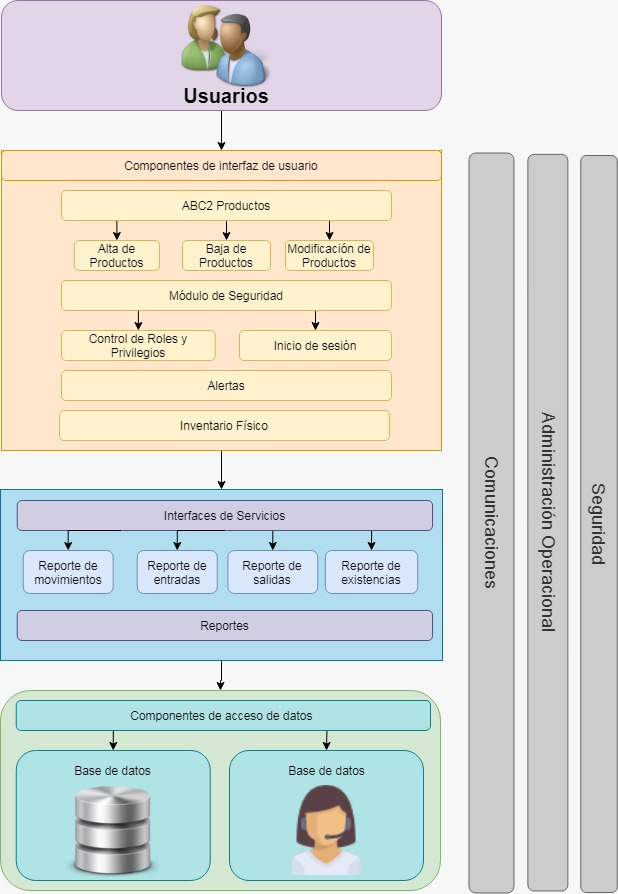
\includegraphics[height=17cm]{ArquitecturaA.jpeg}
%	\caption{Arquitectura a bloques de la aplicación}
%\end{figure}

%\newpage

%\section{Arquitectura de datos}
%\begin{figure}[!htb]
%	\centering
%	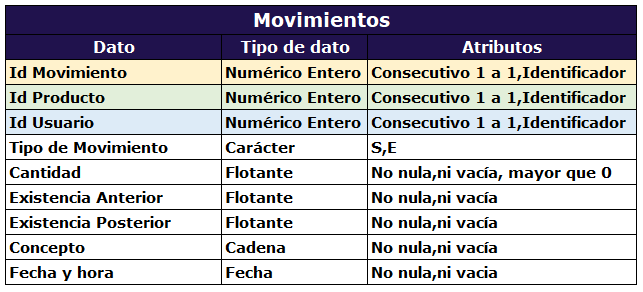
\includegraphics[height=4cm]{MOVIMIENTOS.PNG}
%\end{figure}

%%	\centering
%	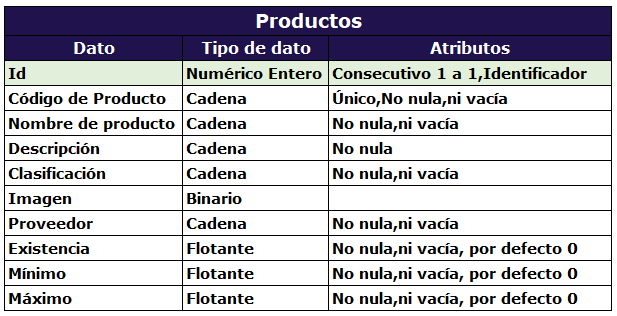
\includegraphics[height=5cm]{PRODUCTOS.PNG}
%\end{figure}

%\begin{figure}[!htb]
%	\centering
%	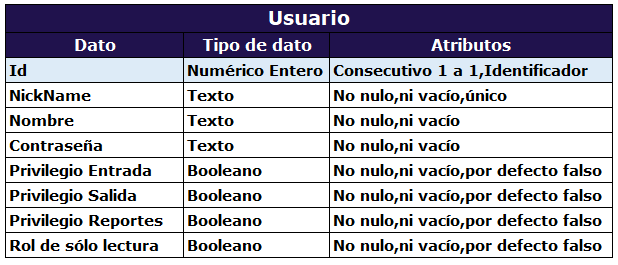
\includegraphics[height=4cm]{USUARIO.PNG}
%\end{figure}

%\begin{figure}[!htb]
%	\centering
%	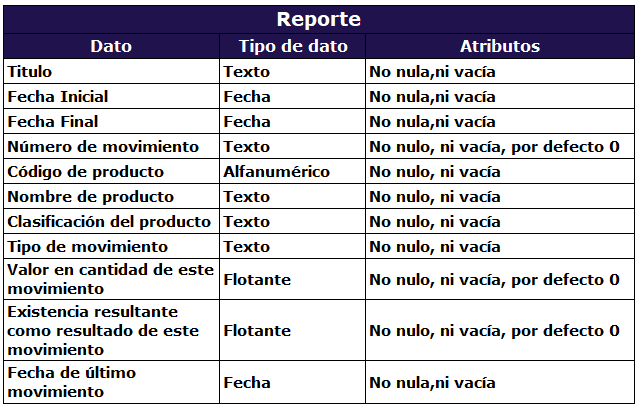
\includegraphics[height=5cm]{REPORTE.PNG}
%\end{figure}

%\newpage

%\section{Prototipos de la aplicación}

%\subsection{Inicio de sesión}
%\begin{figure}[!htb]
%	\centering
%	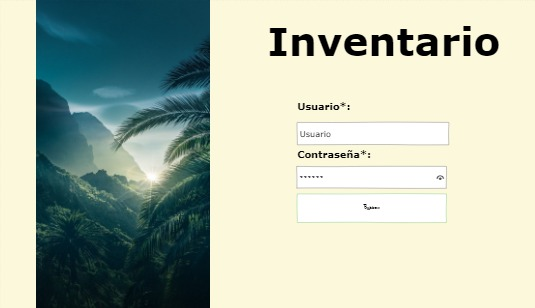
\includegraphics[height=8cm]{Login.jpeg}
%\end{figure}

%\subsection{Pantalla principal de la aplicación}
%%	\centering
%	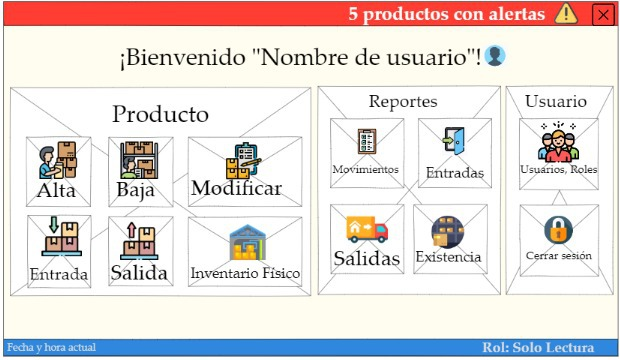
\includegraphics[height=8cm]{Pagina.jpeg}
%\end{figure}

%\newpage
%\subsection{Módulo de seguridad}
%\textbf{Altas,bajas y cambios de usuarios}
%\begin{figure}[!htb]
%	\centering
%	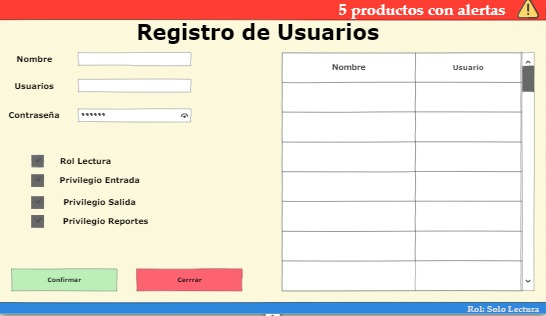
\includegraphics[height=8cm]{AltaUsuarios.jpeg}
%\end{figure}

%\subsection{ABC2 Productos}
%\textbf{Altas,bajas y cambios de productos}
%\begin{figure}[!htb]
%	\centering
%	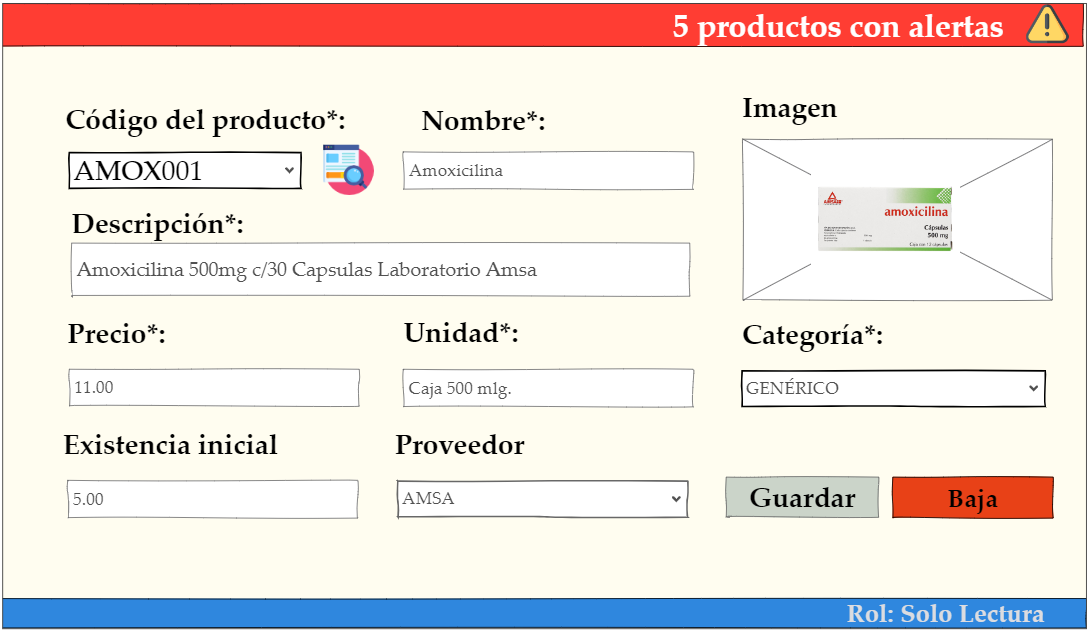
\includegraphics[height=8cm]{Alta.png}
%\end{figure}

%\newpage

%%\textbf{Buscador de productos}
%\begin{figure}[!htb]
%	\centering
%	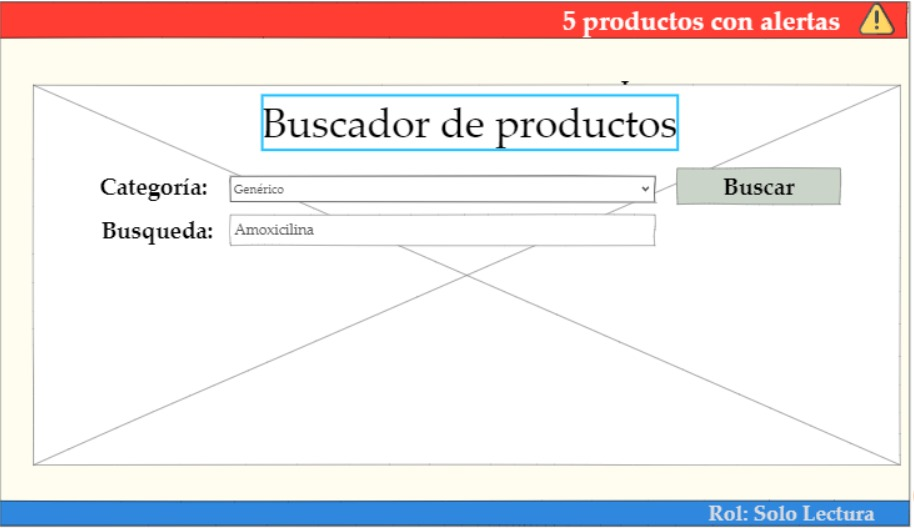
\includegraphics[height=8cm]{Buscador.jpeg}
%\end{figure}


%\subsection{Entrada/Salida de productos}
%\begin{figure}[!htb]
%	\centering
%	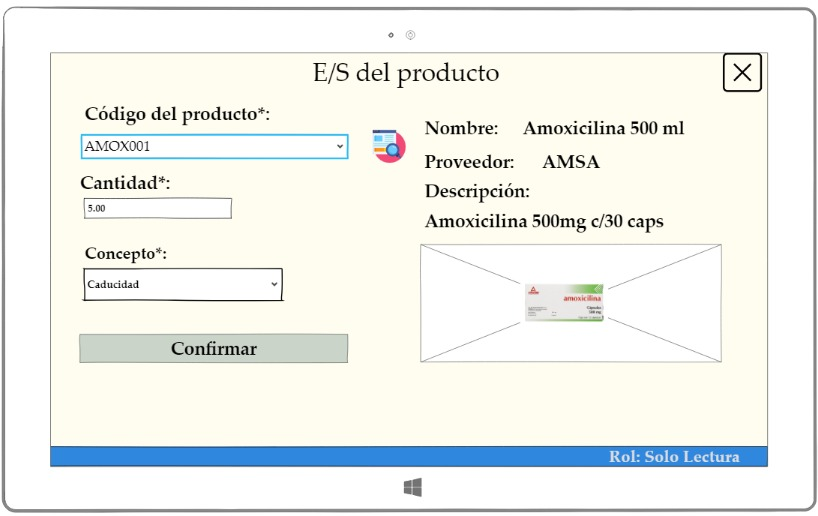
\includegraphics[height=8cm]{ESalidas.jpeg}
%\end{figure}

%\newpage

%\subsection{Inventario Físico vs Teórico}
%\begin{figure}[!htb]
%	\centering
%	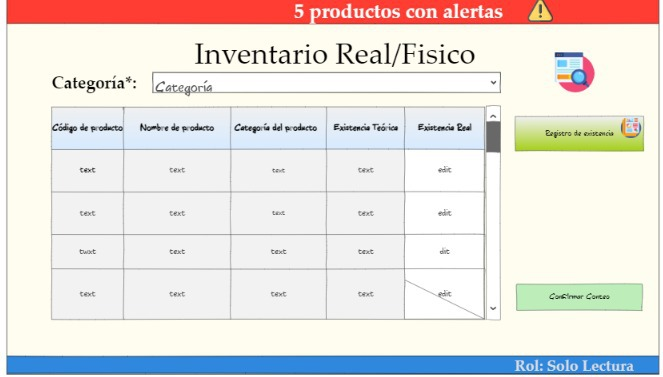
\includegraphics[height=8cm]{Inventario.jpeg}
%\end{figure}
\newpage
\setcounter{chapter}{8}
\setcounter{section}{-1}
\setcounter{subsection}{-1}
\section{Diseños}
\noindent
El diseño del proyecto es el proceso de elaboración de la propuesta de trabajo de acuerdo
a pautas y procedimientos sistemáticos como ya se mencionó, un buen diseño debe identificar a
los beneficiarios y actores claves; establecer un diagnóstico de la situación problema; definir
estrategias posibles para enfrentarla y la justificación de la estrategia asumida; objetivos del
proyecto (generales y específicos); resultados o productos esperados y actividades y recursos
mínimos necesarios.\\
Al mismo tiempo, la propuesta o diseño debe contemplar la definición de indicadores para
realizar el seguimiento y verificación de los resultados que se obtienen, y establecer los factores
externos que garantizan su factibilidad y éxito.\\
Cada uno de los conceptos mencionados: objetivos; estrategia; resultados; productos,
actividades, recursos, indicadores y factores externos, se irán describiendo y analizando por separado, a lo largo del desarrollo del documento y en la medida que avancemos en la elaboración del proyecto.\\
\setcounter{section}{1}
\setcounter{subsection}{-1}
\subsection{Diseño lógico}
El diseño lógico es el proceso de construir un esquema de la información que utiliza la empresa, basándose en un modelo de base de datos específico, independiente del SGBD concreto que se vaya a utilizar y de cualquier otra consideración física.\\
\begin{figure}[!htb]
    \centering
	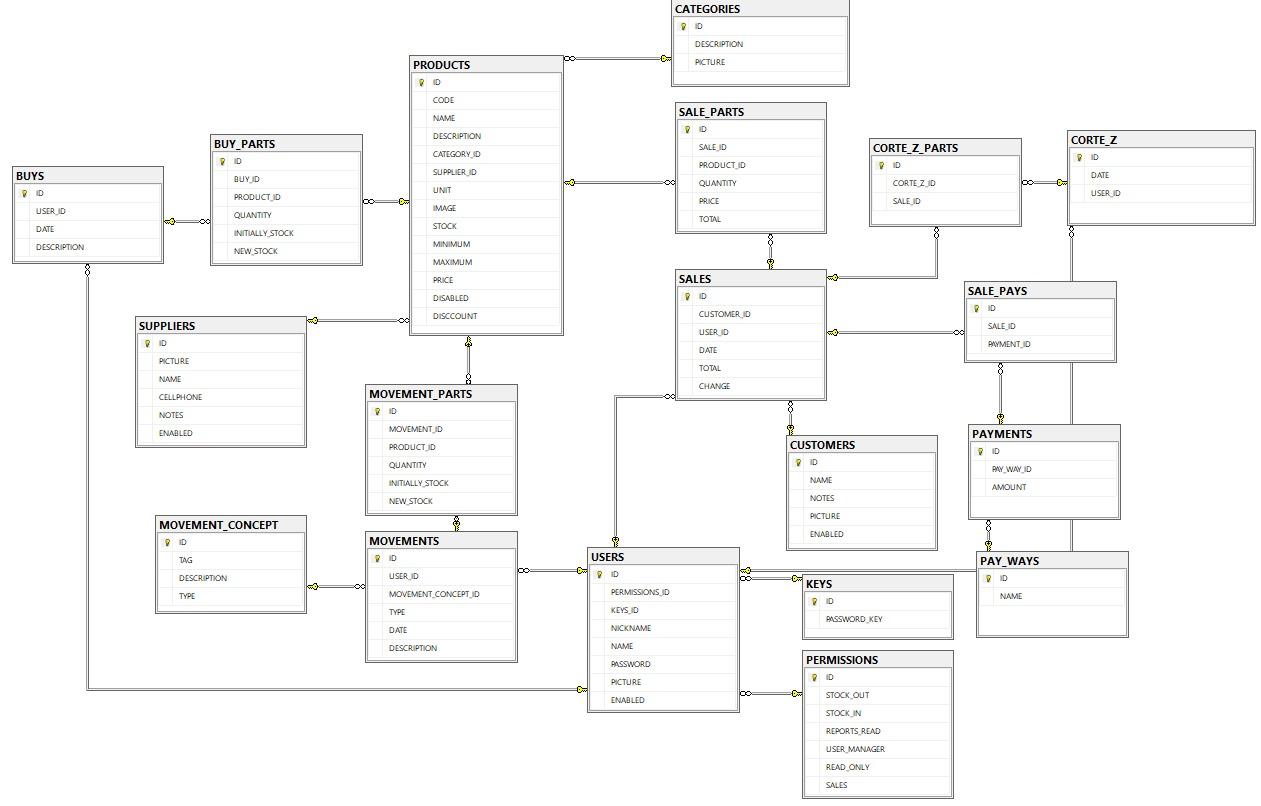
\includegraphics[height=11cm]{Dislogico.jpeg}
\end{figure}
\newpage

\begin{lstlisting}[language={SQL}]
    /* CREA UNA BASE DE DATOS EN BLANCO*/
    CREATE DATABASE DON_CUCO
    GO
    /* UTILIZA ESTA NUEVA BASE DE DATOS*/
    USE DON_CUCO
    GO
    /*ALMACENA LA INFORMACIÓN SOBRE LAS CATEGORIAS DE PRODUCTOS*/
    CREATE TABLE CATEGORIES
    (
      ID INT PRIMARY KEY IDENTITY(1,1),
      DESCRIPTION VARCHAR(100) NOT NULL UNIQUE,
      PICTURE VARCHAR(MAX)
    );
    /*INFORMACIÓN DE PROVEEDORES*/
    CREATE TABLE SUPPLIERS(
        ID INT PRIMARY KEY IDENTITY(1,1),
        PICTURE VARCHAR(MAX),
        NAME VARCHAR(100) NOT NULL,
        CELLPHONE VARCHAR(100),
        NOTES VARCHAR(MAX),
        ENABLED BIT NOT NULL DEFAULT 0
    
    );
    /*INFORMACIÓN DE PRODUCTOS*/
    CREATE TABLE PRODUCTS(
        ID INT PRIMARY KEY IDENTITY(1,1),
        CODE VARCHAR(100) UNIQUE NOT NULL,
        NAME VARCHAR(100) NOT NULL,
        DESCRIPTION VARCHAR(MAX),
        CATEGORY_ID INT FOREIGN KEY REFERENCES CATEGORIES NOT NULL,
        SUPPLIER_ID INT FOREIGN KEY REFERENCES SUPPLIERS NOT NULL,
        UNIT VARCHAR(100) NOT NULL,
        IMAGE VARCHAR(MAX),
        STOCK REAL NOT NULL DEFAULT 0,
        MINIMUM REAL NOT NULL DEFAULT 0,
        MAXIMUM REAL NOT NULL DEFAULT 0,
        PRICE REAL NOT NULL DEFAULT 0,
        DISABLED BIT NOT NULL DEFAULT 0,
        DISCCOUNT INTEGER NOT NULL DEFAULT 0
    );
    /*INFORMACIÓN/MATRIZ DE PERMISOS DE USUARIO*/
    CREATE TABLE PERMISSIONS
    (
        ID INT PRIMARY KEY IDENTITY (1,1),
        STOCK_OUT BIT DEFAULT 0,
        STOCK_IN BIT DEFAULT 0,
        REPORTS_READ BIT DEFAULT 0,
        USER_MANAGER BIT DEFAULT 0,
        READ_ONLY BIT DEFAULT 0,
        SALES BIT DEFAULT 0,
    );
    /* LLAVES,TOKENS DE SEGURIDAD PARA DESENCRIPTAR CONTRASEÑAS DE USUARIO*/
    CREATE TABLE KEYS(
        ID INT PRIMARY KEY IDENTITY(1,1),
        PASSWORD_KEY VARCHAR(37) DEFAULT NEWID()
    );
    /*INFORMACIÓN SOBRE USUARIOS DEL SITEMA */
    CREATE TABLE USERS(
        ID INT PRIMARY KEY IDENTITY(1,1),
        PERMISSIONS_ID INT FOREIGN KEY REFERENCES PERMISSIONS NOT NULL,
        KEYS_ID INT FOREIGN KEY REFERENCES KEYS NOT NULL,
        NICKNAME VARCHAR(100) NOT NULL UNIQUE,
        NAME VARCHAR(100) NOT NULL,
        PASSWORD VARBINARY(MAX) NOT NULL,
        PICTURE VARCHAR(MAX) DEFAULT NULL,
        ENABLED BIT NOT NULL DEFAULT 0
    );
    /*LISTADO DE CONCEPTOS DE MOVIMIENTOS*/
    CREATE TABLE MOVEMENT_CONCEPT
    (
        ID INT PRIMARY KEY IDENTITY(1,1),
        TAG VARCHAR(10) NOT NULL,
        DESCRIPTION VARCHAR(100),
        TYPE VARCHAR(1)
    );
    /*CABECERA DE LA COMPRA*/
    CREATE TABLE BUYS( --1 para que te de el id de movement
        ID INT PRIMARY KEY IDENTITY(1,1),
        USER_ID INT FOREIGN KEY REFERENCES USERS NOT NULL,
        DATE DATETIME NOT NULL DEFAULT GETDATE(),
        DESCRIPTION VARCHAR(100)
    );
    /*PARTIDAS DE LA COMPRA*/
    CREATE TABLE BUY_PARTS(  
        ID INT PRIMARY KEY IDENTITY(1,1),
        BUY_ID INT FOREIGN KEY REFERENCES BUYS NOT NULL,
        PRODUCT_ID INT FOREIGN KEY REFERENCES PRODUCTS NOT NULL,
        QUANTITY REAL NOT NULL DEFAULT 0,
        INITIALLY_STOCK REAL NOT NULL,
        NEW_STOCK REAL NOT NULL
    );
    /*CABECERA DE EL MOVIMIENTO (E/S)*/
    CREATE TABLE MOVEMENTS( --1 para que te de el id de movement
        ID INT PRIMARY KEY IDENTITY(1,1),
        USER_ID INT FOREIGN KEY REFERENCES USERS NOT NULL,
        MOVEMENT_CONCEPT_ID INT FOREIGN KEY REFERENCES MOVEMENT_CONCEPT NOT NULL,
        TYPE VARCHAR(1) NOT NULL,
        DATE DATETIME NOT NULL DEFAULT GETDATE(),
        DESCRIPTION VARCHAR(100)
    );
    /*PARTIDAS DEL MOVIMIENTO*/
    CREATE TABLE MOVEMENT_PARTS(  
        ID INT PRIMARY KEY IDENTITY(1,1),
        MOVEMENT_ID INT FOREIGN KEY REFERENCES MOVEMENTS NOT NULL,
        PRODUCT_ID INT FOREIGN KEY REFERENCES PRODUCTS NOT NULL,
        QUANTITY REAL NOT NULL DEFAULT 0,
        INITIALLY_STOCK REAL NOT NULL,
        NEW_STOCK REAL NOT NULL
    );
    /*REGISTRO DE CLIENTES*/
    CREATE TABLE CUSTOMERS(
        ID INT PRIMARY KEY IDENTITY(1,1),
        NAME VARCHAR(100) NOT NULL,
        NOTES VARCHAR(MAX),
        PICTURE VARCHAR(MAX),
        ENABLED BIT NOT NULL DEFAULT 0
    );
    /*LISTADO DE LAS FORMAS DE PAGO DISPONIBLES*/
    CREATE TABLE PAY_WAYS(	
        ID INT PRIMARY KEY IDENTITY(1,1),
        NAME VARCHAR(50)
    );
    /*LISTADO DE PAGOS RECIBIDOS */
    CREATE TABLE PAYMENTS
    (
        ID INT PRIMARY KEY IDENTITY(1,1),
        PAY_WAY_ID INT FOREIGN KEY REFERENCES PAY_WAYS,
        AMOUNT FLOAT NOT NULL DEFAULT 0
    );
    /*CABECERA DE UNA VENTA*/
    CREATE TABLE SALES(
        ID INT PRIMARY KEY IDENTITY(1,1),
        CUSTOMER_ID INT FOREIGN KEY REFERENCES CUSTOMERS NOT NULL,
        USER_ID INT FOREIGN KEY REFERENCES USERS NOT NULL,
        DATE DATETIME DEFAULT GETDATE(),
        TOTAL REAL,
        CHANGE REAL
    );
    /*PARTIDAS DE UNA VENTA*/
    CREATE TABLE SALE_PARTS(
        ID INT PRIMARY KEY IDENTITY(1,1),
        SALE_ID INT FOREIGN KEY REFERENCES SALES NOT NULL,
        PRODUCT_ID INT FOREIGN KEY REFERENCES PRODUCTS NOT NULL,
        QUANTITY REAL,
        PRICE REAL,
        TOTAL REAL
    );
    /*PAGOS REALIZADOS EN UNA VENTA ESPECIFICA*/
    CREATE TABLE SALE_PAYS(
        ID INT PRIMARY KEY IDENTITY(1,1),
        SALE_ID INT FOREIGN KEY REFERENCES SALES NOT NULL,
        PAYMENT_ID INT FOREIGN KEY REFERENCES PAYMENTS
    );
    GO
    /*REGISTRO DE CORTE DE CAJA DE CIERRE*/
    CREATE TABLE CORTE_Z(
        ID INT PRIMARY KEY IDENTITY(1,1),
        DATE DATETIME,
        USER_ID INT FOREIGN KEY REFERENCES USERS NOT NULL);
    GO
    /*LISTADO DE VENTAS POR CORTE DE CAJA*/
    CREATE TABLE CORTE_Z_PARTS(
        ID INT PRIMARY KEY IDENTITY(1,1),
        CORTE_Z_ID INT FOREIGN KEY REFERENCES CORTE_Z NOT NULL,
        SALE_ID INT FOREIGN KEY REFERENCES SALES NOT NULL,
    );
    GO
    /*REALIZA UN NUEVO CORTE DE CAJA, INSERTA LA LLAVE DE LAS VENTAS QUE PARTICIPAN EN ESTE CORTE*/
    CREATE PROCEDURE SP_CORTE_Z(@USER_ID INT)
    AS
    BEGIN
        DECLARE @CORTE_Z_ID INT
        INSERT INTO CORTE_Z(DATE,USER_ID) VALUES(GETDATE(),@USER_ID);
        SELECT @CORTE_Z_ID=SCOPE_IDENTITY();
        INSERT INTO CORTE_Z_PARTS(CORTE_Z_ID,SALE_ID) SELECT @CORTE_Z_ID,ID FROM SALES WHERE NOT EXISTS 
        (SELECT ID FROM CORTE_Z_PARTS CZ WHERE CZ.SALE_ID=SALES.ID)
        SELECT @CORTE_Z_ID
    END;
    GO
    /*RETORNA UNA VISTA DE LAS VENTAS QUE AÚN NO ESTAN AGRUPADAS EN ALGÚN CORTE DE CAJA*/
    CREATE VIEW VIEW_GETCORTEZ_SALES
    AS
    select SALES.ID,SALES.DATE as 'Fecha',SALES.TOTAL,
    SALES.CHANGE,USERS.NAME as 'User',CUSTOMERS.NAME as 'Customers' 
    From sales
    inner join USERS ON USERS.ID=SALES.USER_ID
    inner join CUSTOMERS ON CUSTOMERS.ID=SALES.CUSTOMER_ID
    WHERE NOT EXISTS 
    (SELECT ID FROM CORTE_Z_PARTS CZ WHERE CZ.SALE_ID=SALES.ID)
    GO
    /*RETORNA UN LISTADO DE LOS PRODUCTOS DE LAS VENTAS QUE AÚN NO ESTAN AGRUPADAS EN ALGÚN CORTE DE CAJA*/
    CREATE VIEW VIEW_GETCORTEZ_PRODUCTS
    AS
    select SALE_ID,NAME,QUANTITY,SALE_PARTS.PRICE,
    TOTAL/1.16 AS 'IMPUESTO',
    TOTAL-TOTAL/1.16 AS 'IMPORTE',
    TOTAL
    From SALE_PARTS
    INNER JOIN PRODUCTS ON PRODUCTS.ID=SALE_PARTS.PRODUCT_ID
    WHERE NOT EXISTS 
    (SELECT ID FROM CORTE_Z_PARTS CZ WHERE CZ.SALE_ID=SALE_PARTS.SALE_ID)
    GO
    /*RETORNA UN LISTADO DE TODOS LOS PAGOS QUE SE HICIERON EN LAS VENTAS QUE AÚN NO ESTAN AGRUPADAS EN ALGÚN CORTE DE CAJA*/
    CREATE VIEW VIEW_PAYMENTS_CORTE_Z
    AS
    select SALE_ID,NAME,AMOUNT
    From SALE_PAYS
    INNER JOIN PAYMENTS ON PAYMENTS.ID=SALE_PAYS.PAYMENT_ID
    INNER JOIN PAY_WAYS ON PAY_WAYS.ID=PAYMENTS.PAY_WAY_ID
    WHERE NOT EXISTS 
    (SELECT ID FROM CORTE_Z_PARTS CZ WHERE CZ.SALE_ID=SALE_PAYS.SALE_ID)
    GO
    /*INSERTA LA CABECERA DE UNA VENTA NUEVA Y RETORNA SU ID*/
    CREATE PROCEDURE SP_SAVE_SALE (@CUSTOMER_ID INT ,@USER_ID INT,@TOTAL FLOAT,@CHANGE FLOAT)
    AS
    BEGIN
    INSERT INTO SALES(CUSTOMER_ID,USER_ID,DATE,TOTAL,CHANGE) VALUES (@CUSTOMER_ID,@USER_ID,GETDATE(),@TOTAL,@CHANGE);
    SELECT SCOPE_IDENTITY();
    END
    GO
    /*INSERTA UNA PARTIDA DE UNA VENTA NUEVA Y RETORNA SU ID*/
    CREATE PROCEDURE SP_SAVE_SALE_PART
    (@SALE_ID INT ,@PRODUCT_ID INT,@PRICE FLOAT,@QUANTITY FLOAT,@TOTAL FLOAT)
    AS
    BEGIN
    --UPDATE PRODUCTS SET STOCK-=@QUANTITY WHERE ID=@PRODUCT_ID 
    INSERT INTO SALE_PARTS
    (SALE_ID,PRODUCT_ID,QUANTITY,PRICE,TOTAL) 
    VALUES (@SALE_ID,@PRODUCT_ID,@QUANTITY,@PRICE,@TOTAL);
    SELECT SCOPE_IDENTITY();
    END
    GO
    /*INSERTA LOS MÉTODOS DE PAGO DE UNA VENTA NUEVA*/
    CREATE PROCEDURE SP_SAVE_SALE_PAYS(@SALE_ID INT,@PAYMENT_ID FLOAT)
    AS
    BEGIN
    INSERT INTO SALE_PAYS(SALE_ID,PAYMENT_ID) VALUES (@SALE_ID,@PAYMENT_ID);
    END
    GO
    /*INSERTA LA CANTIDAD EN DINERO DE UN MÉTODO DE PAGO DE UNA VENTA NUEVA*/
    CREATE PROCEDURE SP_SAVE_PAYMENT(@PAY_WAY_ID INT,@AMOUNT FLOAT)
    AS
    BEGIN
    INSERT INTO PAYMENTS(PAY_WAY_ID,AMOUNT) VALUES (@PAY_WAY_ID,@AMOUNT);
    SELECT SCOPE_IDENTITY();
    END
    GO
    --INSERTA LOS TIPOS DE PAGO POR DEFECTO
    INSERT INTO PAY_WAYS (NAME) VALUES('Cash');
    INSERT INTO PAY_WAYS (NAME) VALUES('Vale');
    INSERT INTO PAY_WAYS (NAME) VALUES('Card');
    --Loguea al usuario pidiendo como parametros Nickname y Password y desencriptando a su vez la contraseña para validarla 
    GO
    CREATE PROCEDURE SP_LOGIN (@NICKNAME VARCHAR(100), @PASSWORD NVARCHAR(50))
    AS
    BEGIN
            DECLARE @USER_ID INT;
            SELECT @USER_ID=ID FROM USERS WHERE NICKNAME=@NICKNAME
            IF(@USER_ID>0)
                BEGIN
                  DECLARE @PASSWORD_KEY VARCHAR(37);
                  DECLARE @REAL_PASSWORD VARCHAR(50);
                  DECLARE @KEY_ID INT;
                  SELECT @KEY_ID=KEYS_ID FROM USERS WHERE ID=@USER_ID
    
                  SELECT @PASSWORD_KEY=PASSWORD_KEY FROM KEYS WHERE ID=@KEY_ID
                  
                  SELECT @REAL_PASSWORD=CONVERT(NVARCHAR(MAX), DECRYPTBYPASSPHRASE(@PASSWORD_KEY, PASSWORD)) FROM USERS WHERE ID=@USER_ID
                  IF (@REAL_PASSWORD=@PASSWORD)
                  BEGIN
                    SELECT 1 AS 'LOGIN_STATUS';
                    RETURN;
                  END
                END
                SELECT 0 AS 'LOGIN_STATUS';
        END;
    GO
    --Registra y/o Actualiza al usuario pidiendo como parametros nickname,contraseña,Nobre y una imagen. 
    --- Encripta la contraseña por seguridad del ususario
    CREATE PROCEDURE SP_REGISTER(@NICKNAME VARCHAR(100), @PASSWORD NVARCHAR(50),@NAME VARCHAR(100),@PICTURE VARCHAR(MAX),@ENABLED BIT,@ID INT)
    AS
    BEGIN
        IF(@ID<=0)
        BEGIN
        DECLARE @PERMISSIONS_ID INT;
        DECLARE @KEY_ID INT;
        DECLARE @KEY VARCHAR(MAX);
        DECLARE @ENCRYPTED_PASSWORD VARBINARY(MAX);
    
        INSERT INTO PERMISSIONS DEFAULT VALUES
        SELECT @PERMISSIONS_ID=SCOPE_IDENTITY();
    
        INSERT INTO KEYS DEFAULT VALUES
        SELECT @KEY_ID=SCOPE_IDENTITY();
        SELECT @KEY =PASSWORD_KEY FROM KEYS WHERE ID=@KEY_ID
    
        SELECT @ENCRYPTED_PASSWORD = ENCRYPTBYPASSPHRASE(@KEY, @PASSWORD);
            
        INSERT INTO USERS(PERMISSIONS_ID,KEYS_ID,NICKNAME,NAME,PASSWORD,PICTURE,ENABLED)
        VALUES(@PERMISSIONS_ID,@KEY_ID,@NICKNAME,@NAME,@ENCRYPTED_PASSWORD,@PICTURE,@ENABLED)
        END ELSE
        BEGIN
    
        SELECT @KEY_ID=KEYS_ID FROM USERS WHERE ID=@ID
        SELECT @KEY =PASSWORD_KEY FROM KEYS WHERE ID=@KEY_ID
        SELECT @ENCRYPTED_PASSWORD = ENCRYPTBYPASSPHRASE(@KEY, @PASSWORD);
        UPDATE USERS SET NICKNAME=@NICKNAME,NAME=@NAME,PASSWORD=@ENCRYPTED_PASSWORD,PICTURE=@PICTURE,ENABLED=@ENABLED
        WHERE ID=@ID
    
        END
    END;
    GO
    
    -------PRODUCTS--------
    GO
    --Obtiene la existencia de un producto mendante su Id
    CREATE PROCEDURE SP_GETSTOCK(@ID INT)
    AS
    BEGIN
    SELECT STOCK FROM PRODUCTS WHERE ID=@ID
    END;
    GO
    ---Obtiene los productos donde DISABLED sea igual a cero y ordnandolos por su nombre
    CREATE PROCEDURE SP_GET_PRODUCTS
    AS
    BEGIN
        SELECT * FROM PRODUCTS WHERE DISABLED=0 ORDER BY NAME
    END;
    GO
    ---Obtiene los productos por su codigo,donde DISABLED sea igual a cero y ordnandolos por su nombre
    CREATE PROCEDURE SP_FIND_PRODUCT(@CODE VARCHAR(100))
    AS
    BEGIN
        SELECT * FROM PRODUCTS WHERE DISABLED=0 AND CODE=@CODE ORDER BY NAME
    END;
    GO
    ---Obtiene todos los productos de la tabla Products
    CREATE PROCEDURE SP_GET_PRODUCT_BY_ID (@ID INT)
    AS
    BEGIN
        SELECT *FROM PRODUCTS WHERE ID=@ID
    END
    GO
    ---Procedure para la busqueda de un producto donde el patrón del codigo o del nombre coincida
    CREATE PROCEDURE SP_SEARCH_PRODUCT(@SEARCH VARCHAR(200))
    AS
    BEGIN
        SELECT * FROM PRODUCTS WHERE DISABLED=0 AND CODE LIKE '%'+@SEARCH+'%' OR NAME LIKE '%'+@SEARCH+'%' ORDER BY NAME
    END;
    GO
    ---Obtiene los productos de una categoria 
    CREATE PROCEDURE SP_GET_PRODUCTS_BY_CATEGORY(@CATEGORY_ID INT)
    AS
    BEGIN
    SELECT * FROM PRODUCTS WHERE DISABLED=0 AND CATEGORY_ID=@CATEGORY_ID ORDER BY NAME
    END;
    GO
    ---Obtiene los productos por la categoria buscada 
    CREATE PROCEDURE SP_GET_PRODUCTS_BY_CATEGORY_FIND(@CATEGORY_ID INT,@SEARCH VARCHAR(MAX))
    AS
    BEGIN
    SELECT * FROM PRODUCTS WHERE DISABLED=0 AND CATEGORY_ID=@CATEGORY_ID AND NAME LIKE '%'+@SEARCH+'%' ORDER BY NAME
    END;
    GO
    --Obtiene las categorias y las ordena por su descripcion
    CREATE PROCEDURE SP_GET_CATEGORIES
    AS
    BEGIN
        SELECT *FROM CATEGORIES order by DESCRIPTION
    END;
    GO
    --Busca las categorias donde el patrón de la descripción categoria o de la descripción del producto coincida ordenandolos por su descripción
    CREATE PROCEDURE SP_FIND_CATEGORIES (@SEARCH VARCHAR(MAX)) 
    AS
    BEGIN
        SELECT DISTINCT CATEGORIES.ID,CATEGORIES.DESCRIPTION FROM CATEGORIES 
        INNER JOIN PRODUCTS ON PRODUCTS.CATEGORY_ID=CATEGORIES.ID
        WHERE CATEGORIES.DESCRIPTION LIKE '%'+@SEARCH+'%' OR PRODUCTS.DESCRIPTION LIKE '%'+@SEARCH+'%' order by CATEGORIES.DESCRIPTION,CATEGORIES.ID
    END;
    GO
    ---Obtiene los categoria por la descripción 
    CREATE PROCEDURE SP_GET_CATEGORY_BY_NAME (@NAME VARCHAR(100))
    AS
    BEGIN
        SELECT *FROM CATEGORIES WHERE DESCRIPTION=@NAME
    END;
    GO
    ---Obtiene los categoria por el Id 
    CREATE PROCEDURE SP_GET_CATEGORY_BY_ID (@ID INT)
    AS
    BEGIN
        SELECT *FROM CATEGORIES WHERE ID=@ID
    END;
    GO
    ---Obtiene todos los provedores de la tabla SUPPLIERS
    CREATE PROCEDURE SP_GET_SUPPLIERS
    AS
    BEGIN
        SELECT *FROM SUPPLIERS
    END;
    GO
    ---Registra y actualizacion de productos con los paramentros de id en caso de actulizar,codigo,nombre,etc...
    CREATE PROCEDURE SP_ABC_PRODUCT (@ID INT,@CODE VARCHAR(100),@NAME VARCHAR(100),@DESCRIPTION VARCHAR(MAX),
    @CATEGORY_ID INT,@SUPPLIER_ID INT,@UNIT VARCHAR(100),@IMAGE VARCHAR(MAX),@STOCK REAL,@MINIMUM REAL,@MAXIMUM REAL,
    @PRICE REAL,@DISABLED BIT,@DISCCOUNT REAL)
    AS
    BEGIN
        IF(@ID<=0)
        BEGIN
            INSERT INTO PRODUCTS (CODE,NAME,DESCRIPTION,CATEGORY_ID,SUPPLIER_ID,UNIT,IMAGE,STOCK,MINIMUM,MAXIMUM,PRICE,DISABLED,DISCCOUNT)
            VALUES(@CODE,@NAME,@DESCRIPTION,@CATEGORY_ID,@SUPPLIER_ID,@UNIT,@IMAGE,@STOCK,@MINIMUM,@MAXIMUM,@PRICE,@DISABLED,@DISCCOUNT)
        END ELSE
        BEGIN
            UPDATE PRODUCTS SET CODE=@CODE,NAME=@NAME,DESCRIPTION=@DESCRIPTION,CATEGORY_ID=@CATEGORY_ID,
            SUPPLIER_ID=@SUPPLIER_ID,UNIT=@UNIT,IMAGE=@IMAGE,STOCK=@STOCK,MINIMUM=@MINIMUM,MAXIMUM=@MAXIMUM,PRICE=@PRICE,DISABLED=@DISABLED,DISCCOUNT=@DISCCOUNT
            WHERE ID=@ID
        END
    END;
    GO
    ---Registra y actualizacion de categosrias con los paramentros de id en caso de actulizar,descripción e imagen
    CREATE PROCEDURE SP_ABC_CATEGORY (@ID INT,@DESCRIPTION VARCHAR(100),@PICTURE VARCHAR(MAX))
    AS
    BEGIN
        IF(@ID<=0)
        BEGIN
            INSERT INTO CATEGORIES(DESCRIPTION,PICTURE) VALUES(@DESCRIPTION,@PICTURE) 
        END ELSE
        BEGIN
            UPDATE CATEGORIES SET DESCRIPTION=@DESCRIPTION,PICTURE=@PICTURE WHERE ID=@ID
        END
    END;
    GO
    ------ALERTS-------
    CREATE VIEW VIEW_OVERSTOCKED
    AS
    SELECT * FROM PRODUCTS WHERE STOCK>=MAXIMUM;
    GO
    CREATE VIEW VIEW_UNDERSTOCKED
    AS
    SELECT * FROM PRODUCTS WHERE STOCK<=MINIMUM;
    GO
    CREATE VIEW VIEW_ALL_ALERTS
    AS
    SELECT * FROM PRODUCTS WHERE STOCK >= MAXIMUM OR STOCK <= MINIMUM;
    GO
    -----MOVEMENTS-----
    GO
    ---Obtiene todos las compras de la tabla BUYS mediante su Id
    CREATE PROCEDURE SP_GET_BUY_BY_ID(@ID INT)
    AS
    BEGIN
    SELECT * FROM BUYS WHERE ID =@ID;
    END;
    GO
    ---Obtiene todos los movimientos de la tabla MOVEMENTS
    CREATE PROCEDURE SP_GET_MOVEMENT(@ID INT)
    AS
    BEGIN
    SELECT * FROM MOVEMENTS WHERE ID =@ID;
    END;
    GO
    ---Obtiene todos las partes de los movimientos de la tabla MOVEMENT_PARTS
    CREATE PROCEDURE SP_GET_MOVEMENTPART_BY_ID(@ID INT)
    AS
    BEGIN
    SELECT * FROM MOVEMENT_PARTS WHERE ID=@ID;
    END;
    GO
    ---Obtiene todos las partes de las compras de la tabla BUY_PARTS
    CREATE PROCEDURE SP_GET_BUY_PART_BY_ID(@ID INT)
    AS
    BEGIN
    SELECT * FROM BUY_PARTS WHERE ID=@ID;
    END;
    GO
    ---Obtiene todos las partes de las compras de la tabla BUY_PARTS ????????? Esta repetido?
    CREATE PROCEDURE SP_GET_BUY_PARTS_BY_ID(@ID INT)
    AS
    BEGIN
    SELECT * FROM BUY_PARTS WHERE BUY_ID=@ID;
    END;
    GO
    ---Obtiene todos las partes de los movimientos de la tabla MOVEMENT_PARTS DADO UN ID DE MOVIMIENTO
    CREATE PROCEDURE SP_GET_MOVEMENTPART(@ID INT)
    AS
    BEGIN
    SELECT * FROM MOVEMENT_PARTS WHERE MOVEMENT_ID=@ID;
    END;
    GO
    ---Obtiene todos los conceptos de la tabla MOVEMENT_CONCEPT 
    CREATE PROCEDURE SP_GET_MOVEMENTCONCEPT(@ID INT)
    AS
    BEGIN
    SELECT * FROM MOVEMENT_CONCEPT WHERE ID =@ID;
    END;
    GO
    ---Registra las compras con los paramentros de id del usuario,fecha y descripción
    CREATE PROCEDURE SP_ADD_BUY(
    @USER_ID INT,
    @DATE DATETIME,
    @DESCRIPTION VARCHAR(100))
    AS
    BEGIN
        INSERT INTO BUYS (USER_ID,DATE,DESCRIPTION)
        VALUES(@USER_ID,@DATE,@DESCRIPTION);
        SELECT SCOPE_IDENTITY();
    END;
    GO
    ---Registra las partes de las compras con los paramentros de id del movimeinto,id del producto y cantidad
    --ademas de que ajusta la existencia de los productos que s even afectados por los movimientos 
    CREATE PROCEDURE SP_ADD_BUY_PARTS(
    @BUY_ID INT,
    @PRODUCT_ID INT,
    @QUANTITY REAL)
    AS
    BEGIN
        DECLARE @INITIALLY_STOCK REAL
        DECLARE @NEW_STOCK REAL
        SELECT @INITIALLY_STOCK = STOCK FROM PRODUCTS WHERE ID=@PRODUCT_ID 
        SELECT @NEW_STOCK=@INITIALLY_STOCK+@QUANTITY
        INSERT INTO BUY_PARTS (BUY_ID,PRODUCT_ID,QUANTITY,INITIALLY_STOCK,NEW_STOCK)
        VALUES(@BUY_ID,@PRODUCT_ID,@QUANTITY,@INITIALLY_STOCK,@NEW_STOCK);
        SELECT SCOPE_IDENTITY();
    END;
    GO
    ---Registra los movimentos con los paramentros de id del usuario,id del concepto,tipo,fecha y descripción
    CREATE PROCEDURE SP_ADD_MOVEMENT(
    @USER_ID INT,
    @MOVEMENT_CONCEPT_ID INT,
    @TYPE VARCHAR(1),
    @DATE_M DATETIME,
    @DESCRIPTION VARCHAR(100))
    AS
    BEGIN
        INSERT INTO MOVEMENTS (USER_ID,MOVEMENT_CONCEPT_ID,TYPE,DATE,DESCRIPTION)
        VALUES(@USER_ID,@MOVEMENT_CONCEPT_ID,@TYPE,@DATE_M,@DESCRIPTION);
        SELECT SCOPE_IDENTITY();
    END;
    GO
    ---Registra las partes de los  movimentos con los paramentros de id del movimeinto,id del producto y cantidad
    --ademas de que ajusta la existencia de los productos que s even afectados por los movimientos 
    CREATE PROCEDURE SP_ADD_MOVENT_PARTS(
    @MOVEMENT_ID INT,
    @PRODUCT_ID INT,
    @QUANTITY REAL,
    @TYPE VARCHAR(1))
    AS
    BEGIN
        DECLARE @INITIALLY_STOCK REAL
        DECLARE @NEW_STOCK REAL
        SELECT @INITIALLY_STOCK = STOCK FROM PRODUCTS WHERE ID=@PRODUCT_ID 
        IF(@TYPE='S')
        BEGIN
            SELECT @QUANTITY=@QUANTITY*-1
        END
        SELECT @NEW_STOCK=@INITIALLY_STOCK+@QUANTITY
        UPDATE PRODUCTS SET STOCK=@NEW_STOCK WHERE ID=@PRODUCT_ID 
        INSERT INTO MOVEMENT_PARTS (MOVEMENT_ID,PRODUCT_ID,QUANTITY,INITIALLY_STOCK,NEW_STOCK)
        VALUES(@MOVEMENT_ID,@PRODUCT_ID,@QUANTITY,@INITIALLY_STOCK,@NEW_STOCK);
        SELECT SCOPE_IDENTITY();
    END;
    GO
    ---Registra los conceptos de movimientos con los paramentros de tag,descripción y tipo
    CREATE PROCEDURE SP_ADD_MOVEMENTCONCEPT(
    @TAG VARCHAR(10),
    @DESCRIPTION VARCHAR(100),
    @TYPE VARCHAR(1))
    AS
    BEGIN
    INSERT INTO MOVEMENT_CONCEPT (TAG,DESCRIPTION,TYPE)
        VALUES(@TAG,@DESCRIPTION,@TYPE);
    END;
    GO
    ---Obtiene todos las compras de la tabla BUYS
    CREATE VIEW VIEW_GET_ALL_BUYS
    AS
    SELECT * FROM BUYS ;
    GO
    ---Obtiene todos los movimientos de la tabla MOVEMENTS
    CREATE VIEW VIEW_GETALLMOVEMENTS
    AS
    SELECT * FROM MOVEMENTS ;
    GO
    ---Obtiene todos los conceptos de movimientos de la tabla MOVEMENT_CONCEPT
    CREATE VIEW VIEW_GETALLMOVEMENTCONCEPT
    AS
    SELECT * FROM MOVEMENT_CONCEPT ;
    GO
    GO
    ---Obtiene todos las partes de los movimientos de la tabla MOVEMENT_PARTS
    CREATE VIEW VIEW_GETALLMOVEMENTPART
    AS
    SELECT * FROM MOVEMENT_PARTS ;
    -----CUSTOMER-----
    GO
    ---Registra y actualizacion de categosrias con los paramentros de id en caso de actulizar,notas e imagen ademas de enabled para eliminar al cliente
    CREATE PROCEDURE SP_ABC_CUSTOMER (@ID INT, @NAME VARCHAR(100),@NOTES VARCHAR(MAX),@PICTURE VARCHAR(MAX),@ENABLED BIT)
    AS
    BEGIN
        IF(@ID<=0)
        BEGIN
            INSERT INTO CUSTOMERS(NAME,NOTES,PICTURE,ENABLED ) VALUES(@NAME,@NOTES,@PICTURE,@ENABLED ) 
        END ELSE
        BEGIN
            UPDATE CUSTOMERS SET NAME= @NAME,NOTES=@NOTES,PICTURE=@PICTURE,ENABLED=@ENABLED  WHERE ID=@ID
        END
    END;
    GO
    ---Obtiene los clientes de la tabla CUSTOMERS mediante su id
    CREATE PROCEDURE SP_SEARCHCUSTOMER(@ID INT)
    AS
    BEGIN
    SELECT * FROM CUSTOMERS WHERE ID= @ID;
    END;
    
    GO
    ---Obtiene todos los clientes de la tabla CUSTOMERS que no esten eliminados
    CREATE VIEW VIEW_GETALL
    AS
    SELECT * FROM CUSTOMERS WHERE ENABLED= 0;
    
    
    -----Supplier----
    GO
    ------Registra y actualizacion de proveedores con los paramentros de id en caso de actulizar,nombre,telefono,etc...
    CREATE PROCEDURE SP_ABC_SUPPLIERS(@ID INT,@NAME VARCHAR(100),@CELLPHONE VARCHAR(100),@NOTES VARCHAR(MAX),@PICTURE VARCHAR(MAX),@ENABLED BIT)
    AS
    BEGIN
        IF(@ID<=0)
        BEGIN
            INSERT INTO SUPPLIERS(NAME,CELLPHONE,NOTES,PICTURE,ENABLED) VALUES (@NAME,@CELLPHONE,@NOTES,@PICTURE,@ENABLED)
        END ELSE
        BEGIN
            UPDATE SUPPLIERS SET NAME=@NAME,CELLPHONE=@CELLPHONE,NOTES=@NOTES,PICTURE=@PICTURE,ENABLED=@ENABLED WHERE ID=@ID;
        END
    END;
    GO
    ---Obtiene a todos los proveedores de la tabla SUPPLIERS
    CREATE VIEW VIEW_GETALLSUPPLIERS
    AS
    SELECT * FROM SUPPLIERS WHERE ENABLED=0;
    GO
    ---Obtiene a  los proveedores de la tabla SUPPLIERS mediante su Id
    CREATE PROCEDURE SP_GETIDSUPPLIERS(@ID INT)
    AS
    SELECT * FROM SUPPLIERS WHERE ID=@ID;
    GO
    /*INSERTA O ACTUALIZA UN DETERMINADO REGISTRO DE PERMISOS GUIANDOSE POR SU ID*/
    CREATE PROCEDURE SP_ABC_PERMISSIONS
    ( @ID INT,@STOCK_OUT BIT,@STOCK_IN BIT ,@REPORTS_READ BIT,@USER_MANAGER BIT,@READ_ONLY BIT,@SALES BIT)
    AS
    BEGIN
    IF(@ID<=0)
    BEGIN
        INSERT INTO PERMISSIONS (STOCK_OUT,STOCK_IN,REPORTS_READ,USER_MANAGER,READ_ONLY,SALES)VALUES(@STOCK_OUT,@STOCK_IN ,@REPORTS_READ ,@USER_MANAGER,
        @READ_ONLY,@SALES)
    END ELSE
    BEGIN
        UPDATE PERMISSIONS SET STOCK_OUT=@STOCK_OUT,STOCK_IN=@STOCK_IN,REPORTS_READ=@REPORTS_READ,USER_MANAGER=@USER_MANAGER,READ_ONLY=@READ_ONLY,SALES=@SALES
        WHERE ID=@ID
    END
    END;
    GO
    /*RECUPERA UN REGISTRO DE PERMISOS POR SU ID*/
    CREATE PROCEDURE GET_PERMISSIONS_BY_ID  (@ID INT)
    AS
    BEGIN
        SELECT *fROM PERMISSIONS WHERE ID=@ID
    END;
    ----USERS-----
    GO
    /*OBTIENE LA INFORMACIÓN UN USUARIO POR SU NICKNAME*/
    CREATE PROCEDURE GET_USER_BY_NICKNAME  (@NICKNAME VARCHAR(100))
    AS
    BEGIN
    
     DECLARE @USER_ID INT;
     SELECT @USER_ID=ID FROM USERS WHERE NICKNAME=@NICKNAME
     DECLARE @PASSWORD_KEY VARCHAR(37);
     DECLARE @REAL_PASSWORD VARCHAR(50);
     DECLARE @KEY_ID INT;
     SELECT @KEY_ID=KEYS_ID FROM USERS WHERE ID=@USER_ID
     SELECT @PASSWORD_KEY=PASSWORD_KEY FROM KEYS WHERE ID=@KEY_ID
     SELECT @REAL_PASSWORD=CONVERT(NVARCHAR(MAX), DECRYPTBYPASSPHRASE(@PASSWORD_KEY, PASSWORD)) FROM USERS WHERE ID=@USER_ID
     SELECT ID,PERMISSIONS_ID,KEYS_ID,NICKNAME,NAME,@REAL_PASSWORD,PICTURE,ENABLED 
     FROM USERS WHERE ID=@USER_ID
    END;
    GO
    /*OBTIENE LA INFORMACIÓN UN USUARIO POR SU ID*/
    CREATE PROCEDURE GET_USER_BY_ID (@ID INT)
    AS
    BEGIN
     DECLARE @PASSWORD_KEY VARCHAR(37);
     DECLARE @REAL_PASSWORD VARCHAR(50);
     DECLARE @KEY_ID INT;
     SELECT @KEY_ID=KEYS_ID FROM USERS WHERE ID=@ID
     SELECT @PASSWORD_KEY=PASSWORD_KEY FROM KEYS WHERE ID=@KEY_ID
     SELECT @REAL_PASSWORD=CONVERT(NVARCHAR(MAX), DECRYPTBYPASSPHRASE(@PASSWORD_KEY, PASSWORD)) FROM USERS WHERE ID=@ID
     SELECT ID,PERMISSIONS_ID,KEYS_ID,NICKNAME,NAME,@REAL_PASSWORD,PICTURE,ENABLED 
     FROM USERS WHERE ID=@ID
    END;
    GO
    GO
    /*RETORNA TODOS LOS USUARIOS QUE NO HAN SIDO ELIMINADOS*/
    CREATE VIEW VIEW_GETALLUSERS
    AS
    SELECT * FROM USERS	WHERE ENABLED=0;
    GO
    /*RETORNA LA INFORMACIÓN DE NOMBRE Y STOCK DE TODOS LOS PRODUCTOS*/
    CREATE VIEW VIEW_GET_STOCK
    AS
    SELECT 
    code,NAME,stock,MINIMUM,MAXIMUM
    FROM products where DISABLED=0
    GO 
    /*RETORNA UN REPORTE DE VENTAS ENTRE UN RANGO DE FECHAS O BIEN TODOS LOS REGISTROS*/
    CREATE PROCEDURE SALES_REPORT(@BEGIN DATETIME,@END DATETIME,@ALL BIT)
    AS
    BEGIN
    select SALES.ID,SALES.DATE as 'Fecha',SALES.TOTAL,SALES.CHANGE,USERS.NAME as 'User',CUSTOMERS.NAME as 'Customers' 
    From sales
    inner join USERS ON USERS.ID=SALES.USER_ID
    inner join CUSTOMERS ON CUSTOMERS.ID=SALES.CUSTOMER_ID
    WHERE @ALL=1 OR (SALES.DATE>=@BEGIN AND SALES.DATE<=@END)
    END
    GO
    /*RETORNA UN REPORTE DE MOVIMIENTOS POR USUARIO ENTRE UN RANGO DE FECHAS O BIEN TODOS LOS REGISTROS*/
    CREATE PROCEDURE SP_MOVENTS_REGISTER (@BEGIN DATETIME,@END DATETIME,@ALL BIT)
    AS
    BEGIN
    SELECT 'Ticket #'+CAST(SALES.ID AS VARCHAR(MAX)) AS ID,USERS.NAME, DATE AS 'Fecha' ,'Venta'AS TYPE FROM SALES
    INNER JOIN USERS ON USERS.ID=SALES.USER_ID
    WHERE @ALL=1 OR (SALES.DATE>=@BEGIN AND SALES.DATE<=@END)
    UNION 
    SELECT 'Movimiento #'+CAST(MOVEMENTS.ID AS VARCHAR(MAX)) as ID,USERS.NAME, DATE AS 'Fecha',
    IIF(TYPE='S','Salida','Entrada') AS TYPE  
    FROM MOVEMENTS
    INNER JOIN USERS ON USERS.ID=MOVEMENTS.USER_ID
    WHERE @ALL=1 OR (MOVEMENTS.DATE>=@BEGIN AND MOVEMENTS.DATE<=@END)
    UNION 
    SELECT 'Compra #'+CAST(BUYS.ID AS VARCHAR(MAX)) as ID,USERS.NAME, DATE AS 'Fecha','Compra' AS TYPE  
    FROM BUYS
    INNER JOIN USERS ON USERS.ID=BUYS.USER_ID
    WHERE @ALL=1 OR (BUYS.DATE>=@BEGIN AND BUYS.DATE<=@END)
    END;
\end{lstlisting}

\subsection{Ejemplo de llamada a procedimiento}

\begin{lstlisting}[language={[Sharp]C}]
    AppData.SQL.EXEC("SP_ABC_PRODUCT", CommandType.StoredProcedure,
    new SqlParameter("ID", Id),
    new SqlParameter("CODE", Code),
    new SqlParameter("NAME", Name),
    new SqlParameter("DESCRIPTION", Description),
    new SqlParameter("CATEGORY_ID", Category.Id),
    new SqlParameter("SUPPLIER_ID", Supplier.Id),
    new SqlParameter("STOCK", Stock),
    new SqlParameter("UNIT", Unit),
    new SqlParameter("IMAGE", Picture),
    new SqlParameter("MINIMUM", Minimum),
    new SqlParameter("MAXIMUM", Maximum),
    new SqlParameter("PRICE", Price),
    new SqlParameter("DISABLED", Disabled),
    new SqlParameter("DISCCOUNT", Disccount)
    );

    using (IReader reader = AppData.SQL.Read("SP_GET_PRODUCT_BY_ID", CommandType.StoredProcedure, 
    new SqlParameter("ID", Id)))
{
    if (reader.Read())
    {
        producto = new Product()
        {
            Id = Convert.ToInt32(reader[0]),
            Code = Convert.ToString(reader[1]),
            Name = Convert.ToString(reader[2]),
            Description = Convert.ToString(reader[3]),
            Category = Category.GetById(Convert.ToInt32(reader[4])),
            Supplier = Supplier.GetById(Convert.ToInt32(reader[5])),
            Unit = Convert.ToString(reader[6]),
            Picture = reader[7].ToString(),
            Stock = Convert.ToSingle(reader[8]),
            Minimum = Convert.ToSingle(reader[9]),
            Maximum = Convert.ToSingle(reader[10]),
            Price = Convert.ToSingle(reader[11]),
            Disabled = Convert.ToBoolean(reader[12]),
            Disccount = Convert.ToInt32(reader[13])
        };
    }
}
\end{lstlisting}


\newpage
\setcounter{section}{2}
\setcounter{subsection}{-1}
\subsection{Diseño conceptual}

		\begin{figure}[h!]
		\centering
		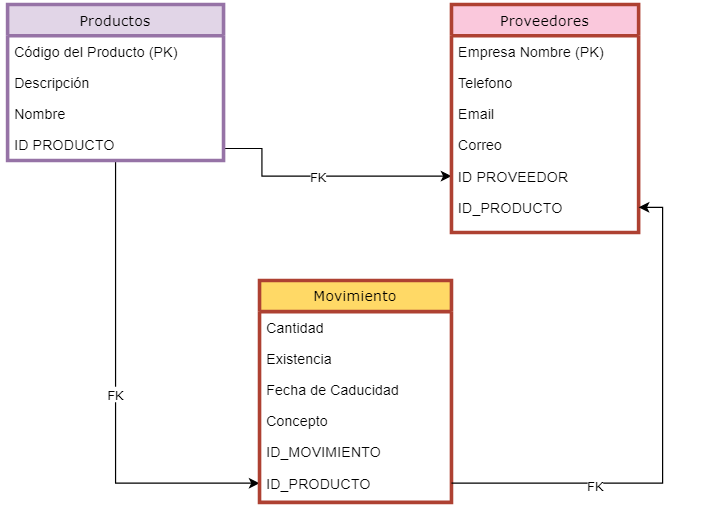
\includegraphics[scale=0.4]{Version 1 tabla.PNG}
		\caption{Primera Versión tabla 1}
		\end{figure}
		
		\begin{figure}[h!]
		\centering
		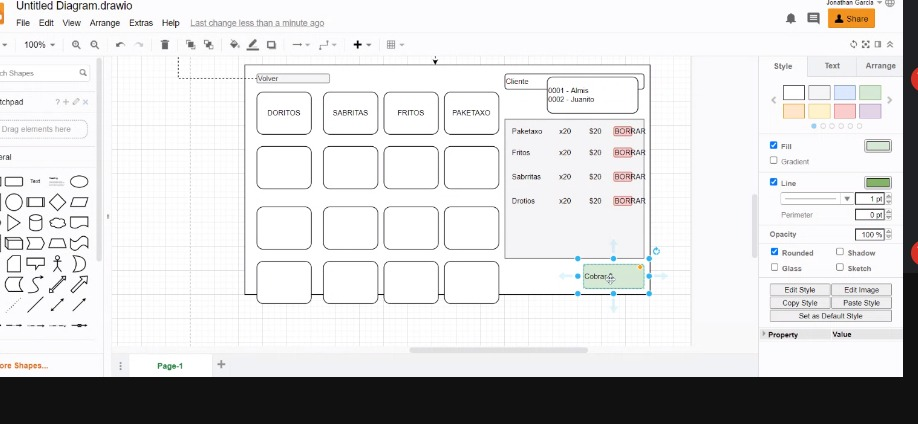
\includegraphics[scale=0.4]{boceto 1.jpg}
		\caption{Boceto Productos}
		\end{figure}
		
		
		\begin{figure}[h!]
		\centering
		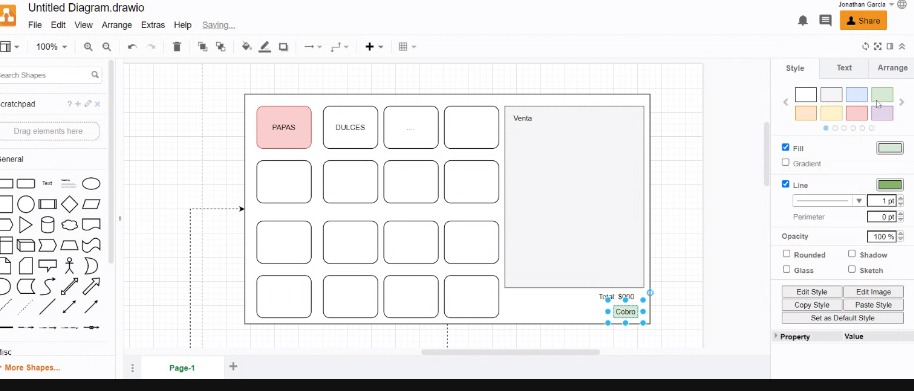
\includegraphics[scale=0.4]{boceto 2.jpg}
		\caption{Boceto Productos}
		\end{figure}
		
		\begin{figure}[h!]
		\centering
		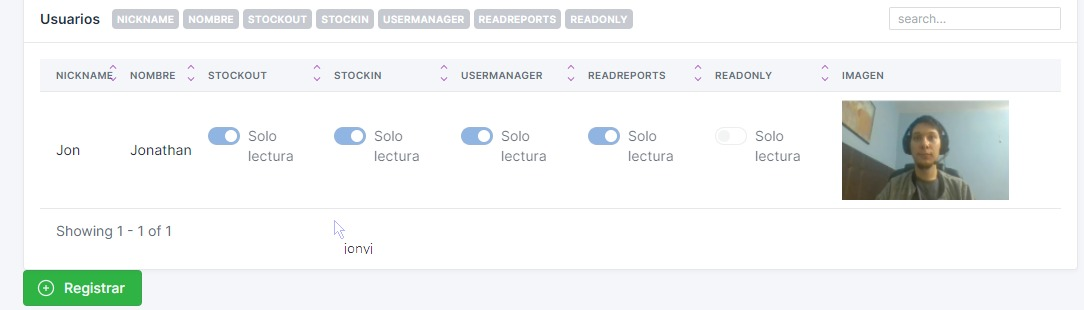
\includegraphics[scale=0.4]{boceto 3.jpg}
		\caption{Boceto final de usuarios}
		\end{figure}



%%%%%%%%%%END DISEÑOS

%%%%%%%%%%%BEGIN MANUALES
\newpage
\setcounter{chapter}{9}
\setcounter{section}{-1}
\setcounter{subsection}{-1}
\section{Manual de usuario}
\noindent

\section{Introducción}


 El aplicativo web es un software que permite a nuestros clientes realizar el almacenamiento y la consulta de los datos registrados en la base de datos. Nos permitirá tomar el control de cada producto que se vaya ingresando de los proveedores, así como los productos que vayan de salida de cada cliente.

\subsection{¿Cómo usar este manual?} La interface principal presenta la opción para que ingrese el nombre, contraseña y tipo de usuario. Entre las opciones principales constarán las siguientes: 
 
\begin{itemize}
    \item Módulo Administrador
    \item Módulo Usuario
\end{itemize}

Cuando se ingresa a cualquiera de las opciones anteriormente mencionadas se podrá escoger entre varias funciones, todo esto referente a la opción escogida. 



\clearpage

\section{Visión general de la aplicación}
\subsection{Entrada al sistema} 
Para poder entrar en la aplicación es obligatorio identificarse, para ello es necesario introducir el usuario y la contraseña.

	\begin{figure}[!htb]
		\centering
		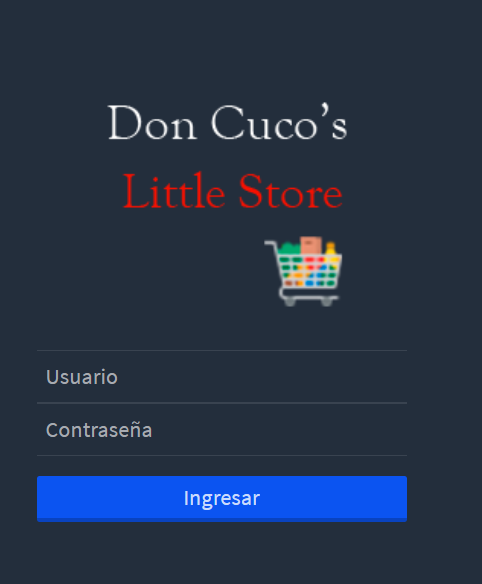
\includegraphics[scale=0.4]{Login.PNG}
		\caption{Ingreso de Usuario y contraseña}
	\end{figure}

 Botones disponibles:\\

Ingresar:  Una vez introducido el usuario y la contraseña, pulsar este botón para acceder al menú principal dónde una vez dentro del sistema se nos desplegara una vista.
\clearpage

\section{Menú del sistema}

	\begin{figure}[!htb]
		\centering
		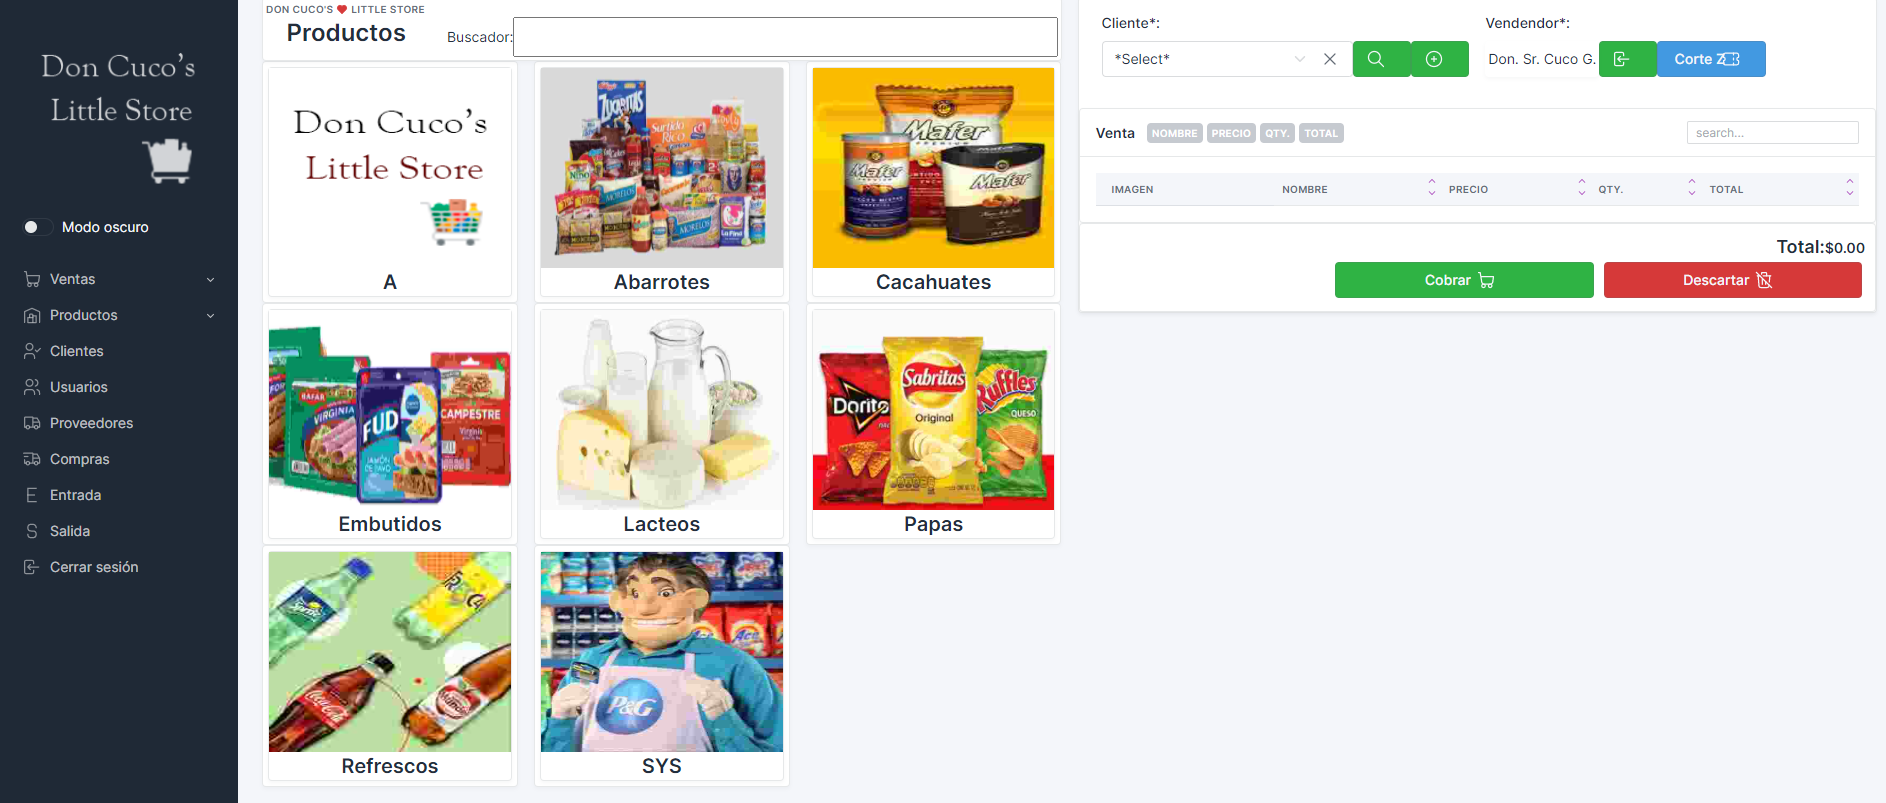
\includegraphics[scale=0.3]{VENTAS.PNG}
		\caption{Menú en la Parte de Productos}
	\end{figure}

	\begin{figure}[!htb]
		\centering
		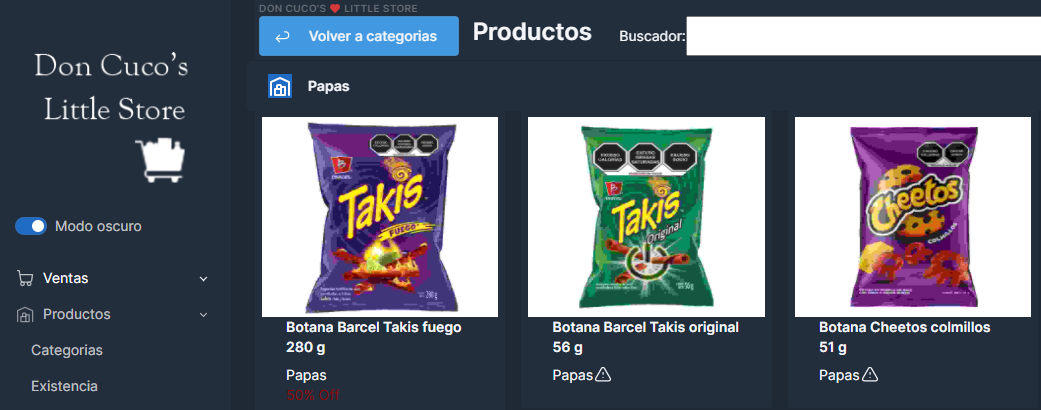
\includegraphics[scale=0.4]{TEMAOSCURO.PNG}
		\caption{Vista de tema oscuro}
	\end{figure}
	
En esta parte podemos ver que tenemos acceso a diferentes partes de la aplicación:\\
\clearpage 

\subsection{Ventas}

	\begin{figure}[!htb]
		\centering
		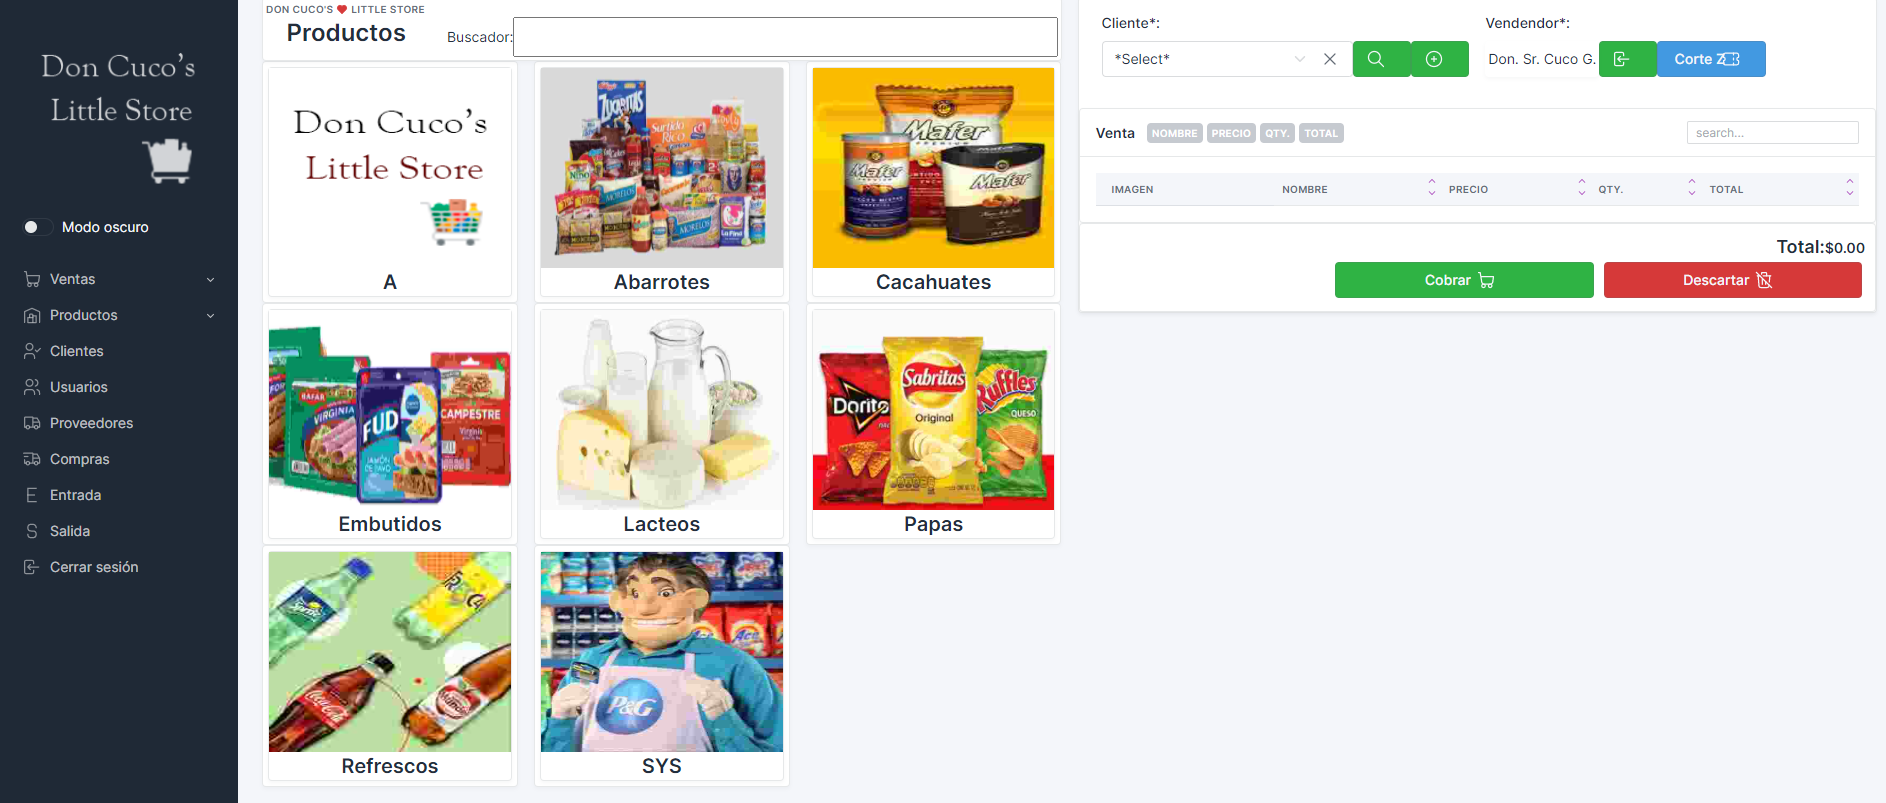
\includegraphics[scale=0.3]{VENTAS.PNG}
		\caption{Vista de ventas}
	\end{figure}
	
Se tiene una ventana la cual estará divida en dos partes:
\begin{itemize}


	\item En una parte se encuentran los accesos de rápido de categorías de los productos que se venden en la tienda. 
	\item Al dar clic a la categoría de elección, esta mitad de pantalla cambiará para mostrar los productos que se encuentran dentro de la categoría previamente seleccionada.
	\end{itemize}
	
	\clearpage
	
	\begin{figure}[!htb]
		\centering
		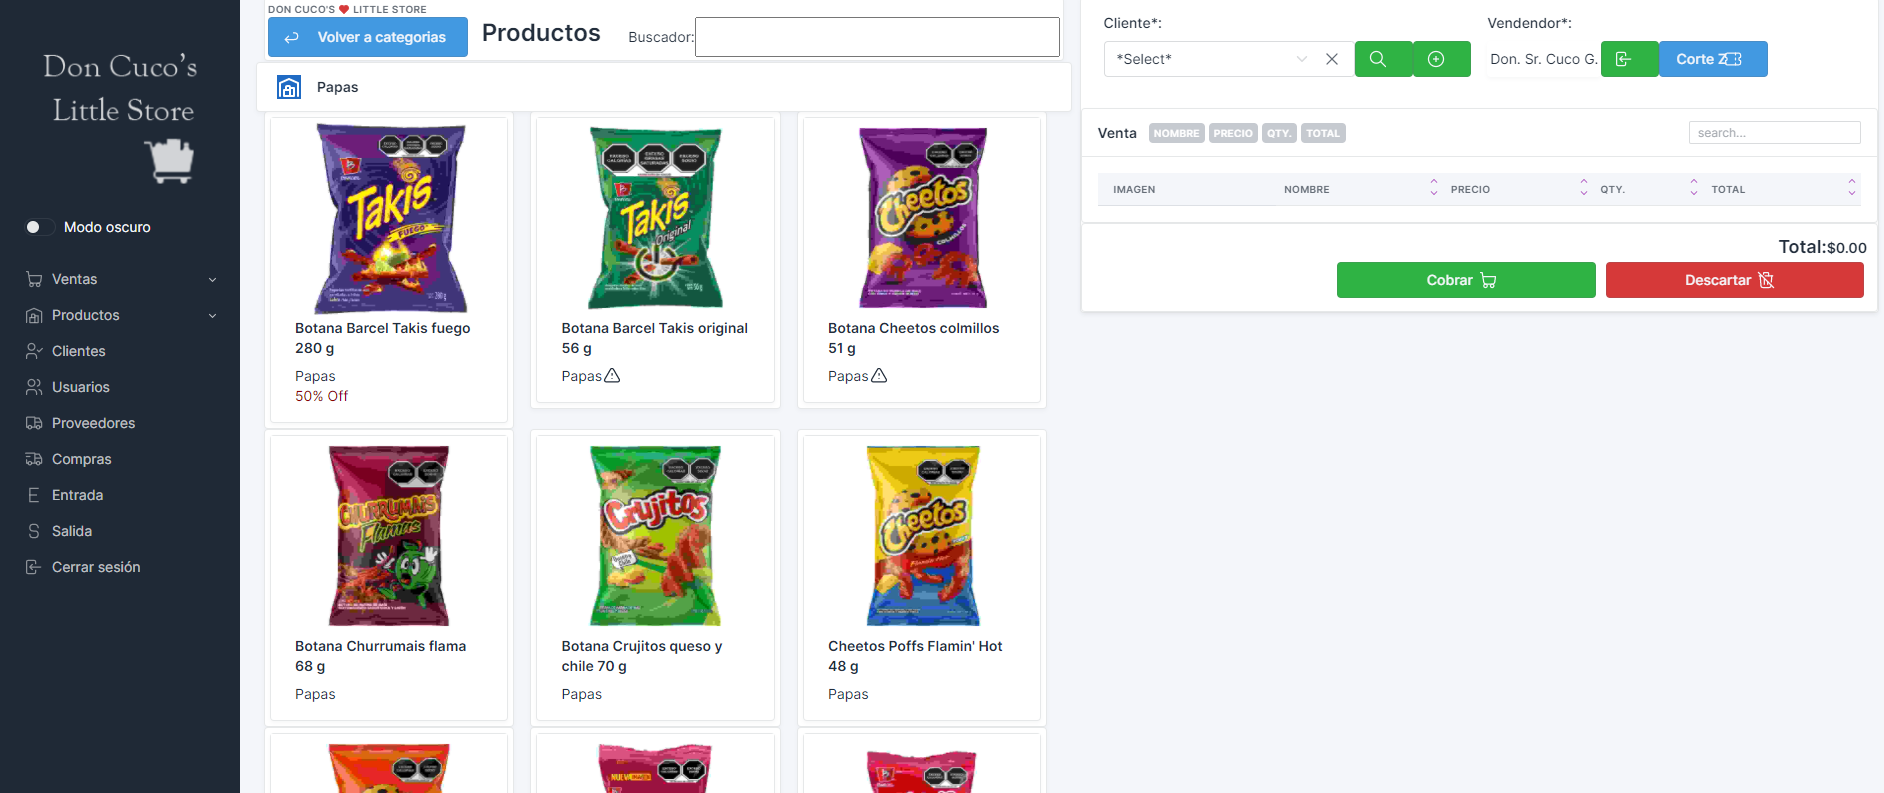
\includegraphics[scale=0.4]{VENTAS1.PNG}
		\caption{Vista de Categoría de Papas}
	\end{figure}
	
	Al estar dentro de una categoría seleccionada, en la parte superior izquierda, habrá un botón de diga “volver a las categorías” para regresar al menú de categorías.\\
	
	\begin{figure}[!htb]
		\centering
		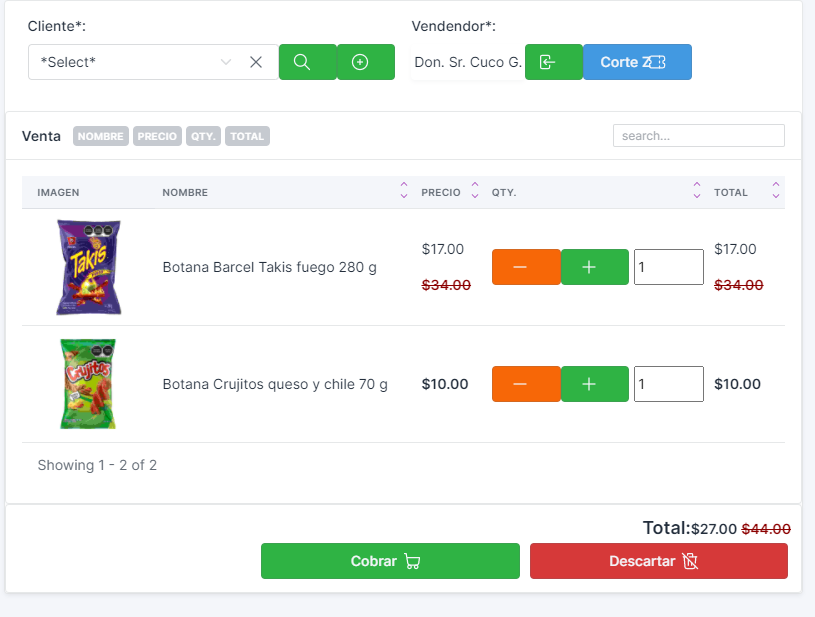
\includegraphics[scale=0.4]{VENTAS2.PNG}
		\caption{Vista de seleccion de productos}
	\end{figure}
	\clearpage
	En esta vista se encuentra: \\
	Cliente: Es una lista desplegable, en la cual se puede seleccionar el cliente a quien se le esté realizando una venta. Para hacer más fácil la búsqueda de un cliente ya existente, hay un botón de “lupa” del lado derecho, en donde al dar clic, se puede ingresar el nombre del cliente a buscar. En caso de no existir el nombre en la Base de Datos, se puede agregar un nuevo cliente, dando clic en el botón “más”.\\
	
     Vendedor: Sirve para seleccionar el nombre del vendedor que en ese momento esté realizando una venta.\\
  
    Venta: Es una sección en donde al seleccionar un producto (de la otra mitad que se mencionó anteriormente), la información de dicho producto se verá reflejada en esta sección. En caso de no querer seleccionar por medio del menú que se muestra en la otra mitad de la pantalla, se cuenta con un campo “search” para poder buscar el producto por su nombre. La búsqueda irá filtrando lo que encuentre registrado en la base de datos con la palabra o las palabras ingresadas. cuenta con los campos de: Imagen, Nombre, Precio, Cantidad y Total.\\

	
	\begin{figure}[!htb]
		\centering
		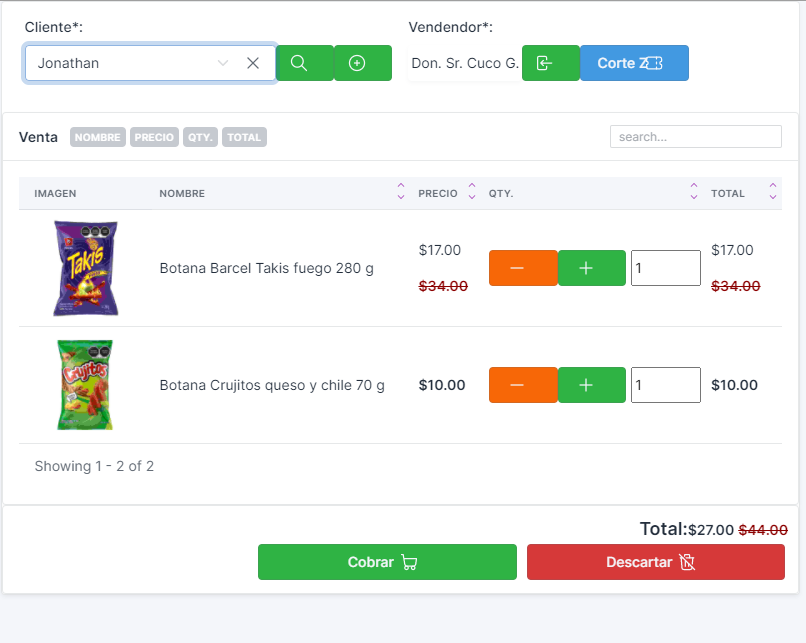
\includegraphics[scale=0.4]{VENTAS3.PNG}
		\caption{Cobro de productos}
	\end{figure}	
	
	\begin{figure}[!htb]
		\centering
		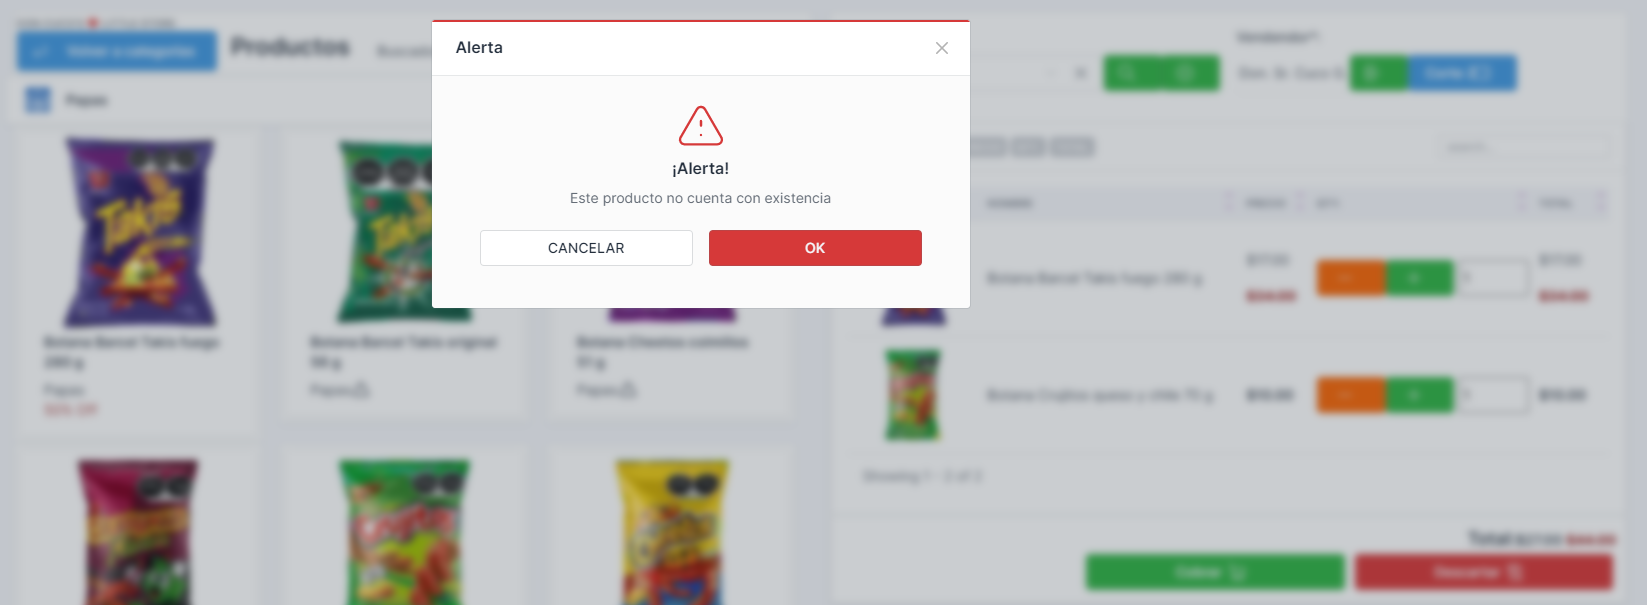
\includegraphics[scale=0.4]{VENTAS4.PNG}
		\caption{Ventana de Alerta}
	\end{figure}
	
	En esta ventana se abrirá cuándo se selecciona un producto que no hay en existencia.\\
	 Aquí se encuentran dos botones:\\
	Cancelar: Cancelara la opción que se haya seleccionado\\
	Ok: Cerrará la ventana \\
	\begin{figure}[!htb]
		\centering
		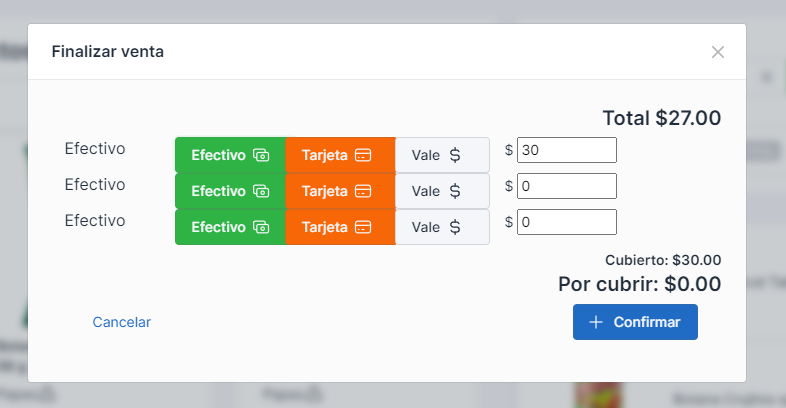
\includegraphics[scale=0.4]{VENTAS8.PNG}
		\caption{Ventana de cobro}
	\end{figure}
	Aquí se abrirá una ventana de confirmación de los productos seleccionados para la venta\\
	\begin{itemize}
	
	\item Tenemos los siguientes botones:
	\item Cancelar: Cancelara la opción de cobro
	\item Confirmar: Confirmará la venta de los productos seleccionados y de cobrará y abrirá lo siguiente:
	    
	\end{itemize}
	
	\begin{figure}[!htb]
		\centering
		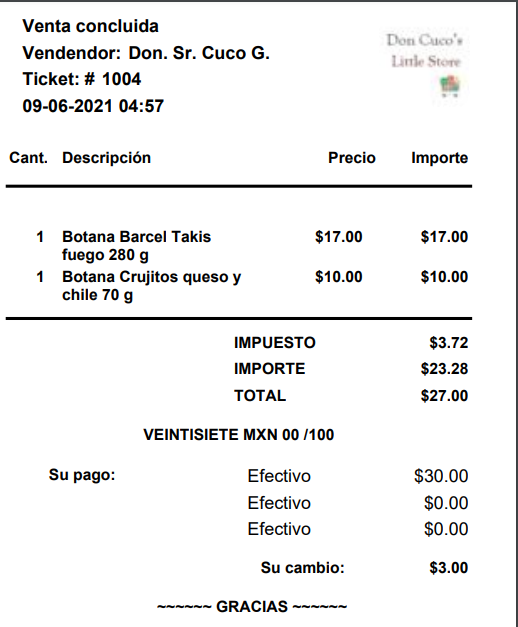
\includegraphics[scale=0.4]{VENTAS9.PNG}
		\caption{Ticket de venta realizada}
	\end{figure}
Se confirma la venta realizada de los productos realizados\\
	
\subsection{Productos}
 Esta parte de la aplicación abrirá la sección de productos y sus categorías que hay de estos mismos.\\
	
	\begin{figure}[!htb]
		\centering
		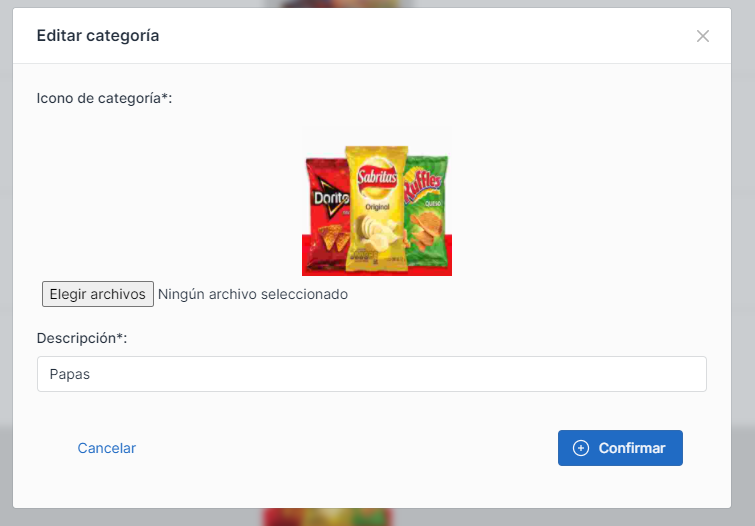
\includegraphics[scale=0.4]{ALTACATEGORIA.PNG}
		\caption{Ventana de Alta de una Categoría}
	\end{figure}
	
	En esta ventana se abrirá cuándo queramos dar de alta una categoría diferente que tengamos en nuestra tienda.\\
	
	Cuenta con las siguientes opciones:\\
	\begin{itemize}
	\item Elegir archivos: Vista previa que tendremos para seleccionar más rápido un producto a la hora de venta
	\item Descripción: Una breve descripción de lo que es la categoría
	\item Cancelar: Cancelará la opción d edar de alta un producto
	\item Confirmar: Se creará la nueva categoría en nuestro sistema
	\end{itemize}
		\begin{figure}[!htb]
		\centering
		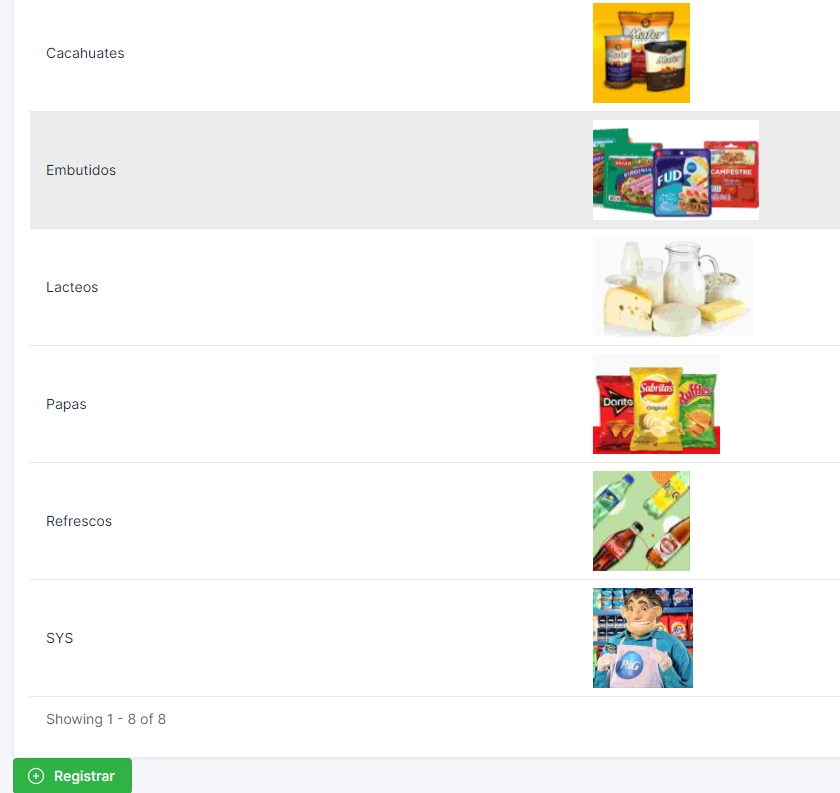
\includegraphics[scale=0.4]{CATEGORIAS.PNG}
		\caption{Categorías de los Productos}
	\end{figure}
	Diferentes productos que podemos tener en nuestra aplicación\\
	
		\begin{figure}[!htb]
		\centering
		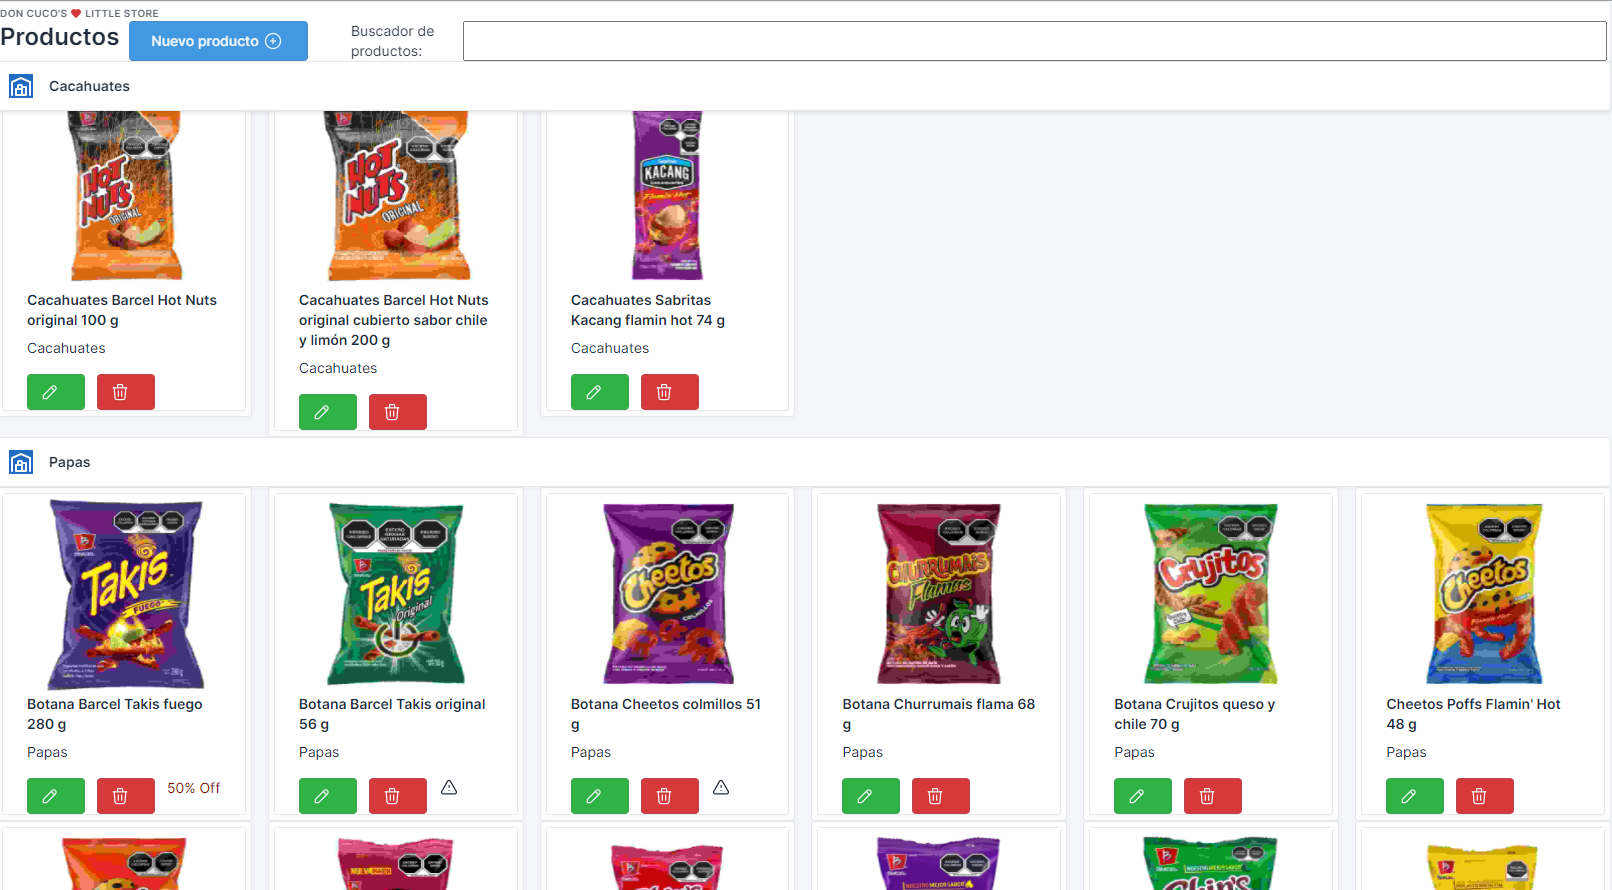
\includegraphics[scale=0.4]{PRODUCTOS1.PNG}
		\caption{Vista de productos seleccionados ya caducados}
	\end{figure}
	
	\clearpage
	
\subsection{Clientes}

	
	\begin{figure}[!htb]
		\centering
		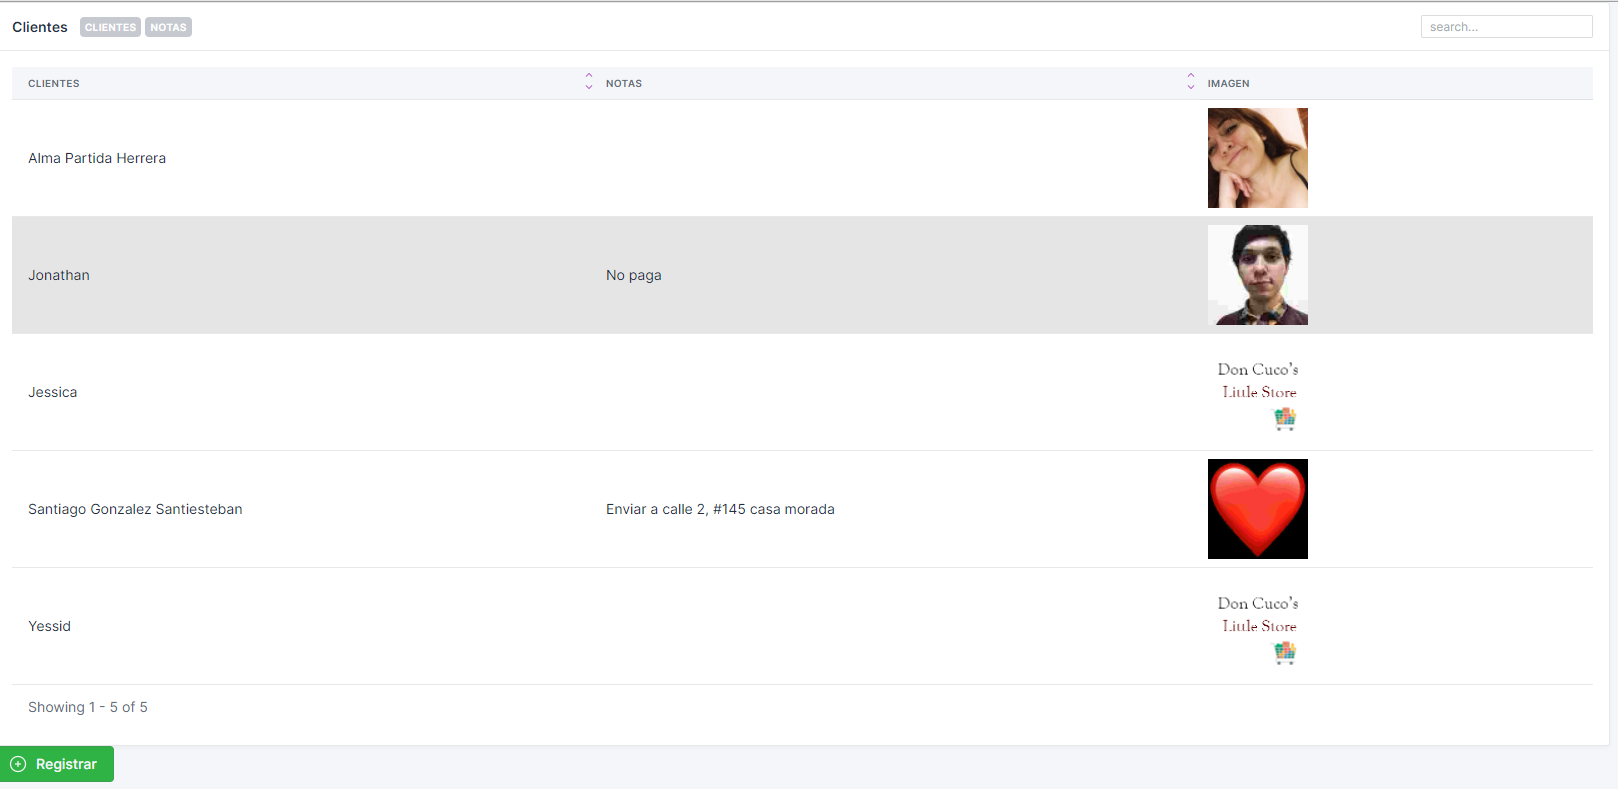
\includegraphics[scale=0.4]{CLIENTES.PNG}\\
		\caption{Vista general de nuestros clientes}
	\end{figure}
	Aquí encontraremos nuestra sección de clientes de nuestro menú este cuenta con un boton de registrar que nos abrirá la siguiente ventana:\\

	
		\begin{figure}[!htb]
		\centering
		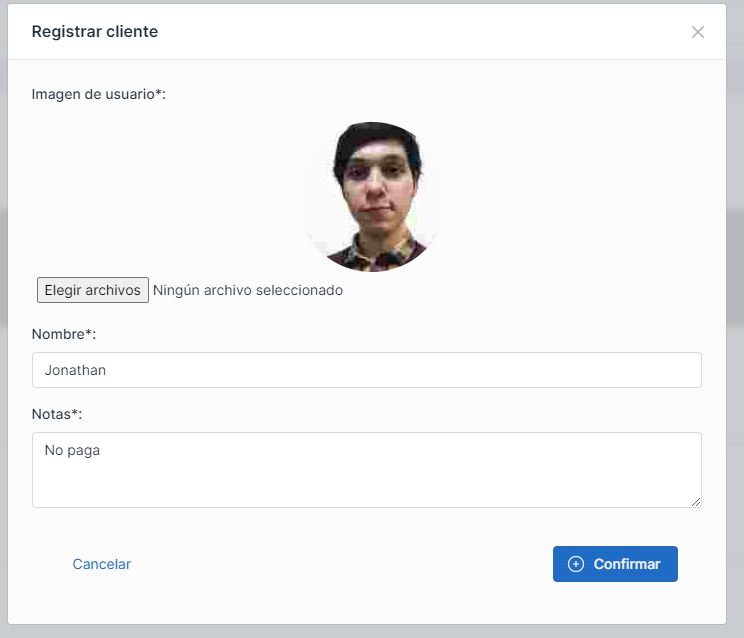
\includegraphics[scale=0.4]{REGISTRARCLIENTE.PNG}\\
		\caption{Ventana para dar de alta a un cliente}
	\end{figure}
'
	 Esta ventana tiene los siguientes botones:\\
	 \begin{itemize}
	\item Elegir archivo: Podremos subir una imagen para identificar nuestros clientes
	\item Nombre: En esta se pondrá el nombre de nuestros clientes 
	\item Cancelar: Cancelará la alta de un cliente
	\item Confirmar: Dará de alta nuestro cliente que queramos registrar
	\end{itemize}


\subsection{Usuarios}

	\begin{figure}[!htb]
		\centering
		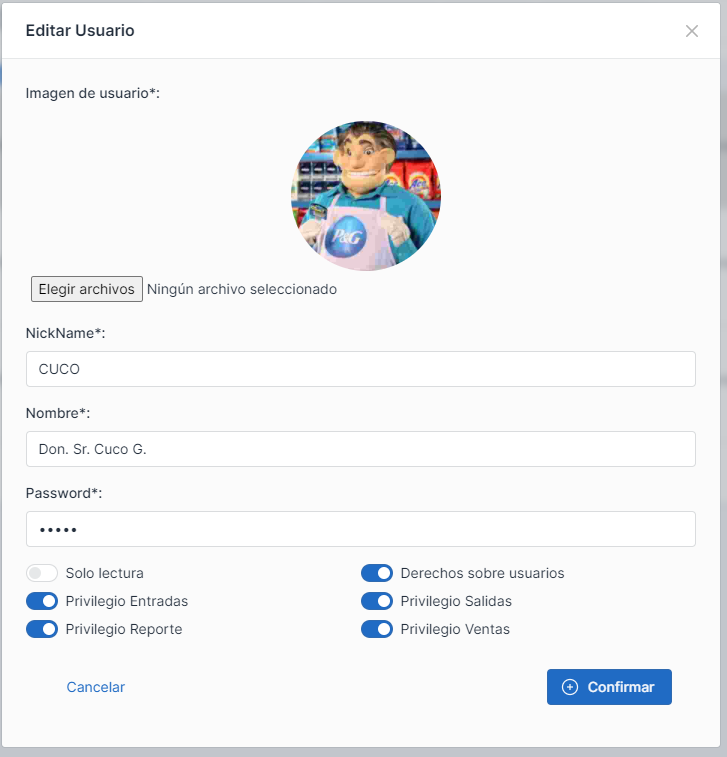
\includegraphics[scale=0.4]{ALTAUSUARIO.PNG}\\
		\caption{Ventana de Dar de alta un usuario}
	\end{figure}
	En esta parte se definirán los roles y privilegios que tendrán nuestros usuarios que vayan atender.\\
	\\ En esta parte damos de alta a nuestros usuarios, al igual cuenta con una opción para definir una imagen y nos sea más fácil identificar.
\begin{itemize}
	\item Elegir archivos: Vista previa de imagen de nuestro usuario
	\item Nombre: Nombre de nuestro usuario
	\item Botones de privilegios:
	\item Cancelar: Cancelará la opción d edar de alta un producto
	\item Confirmar: Se creará la nueva categoría en nuestro sistema
\end{itemize}
	
	
		\begin{figure}[!htb]
		\centering
		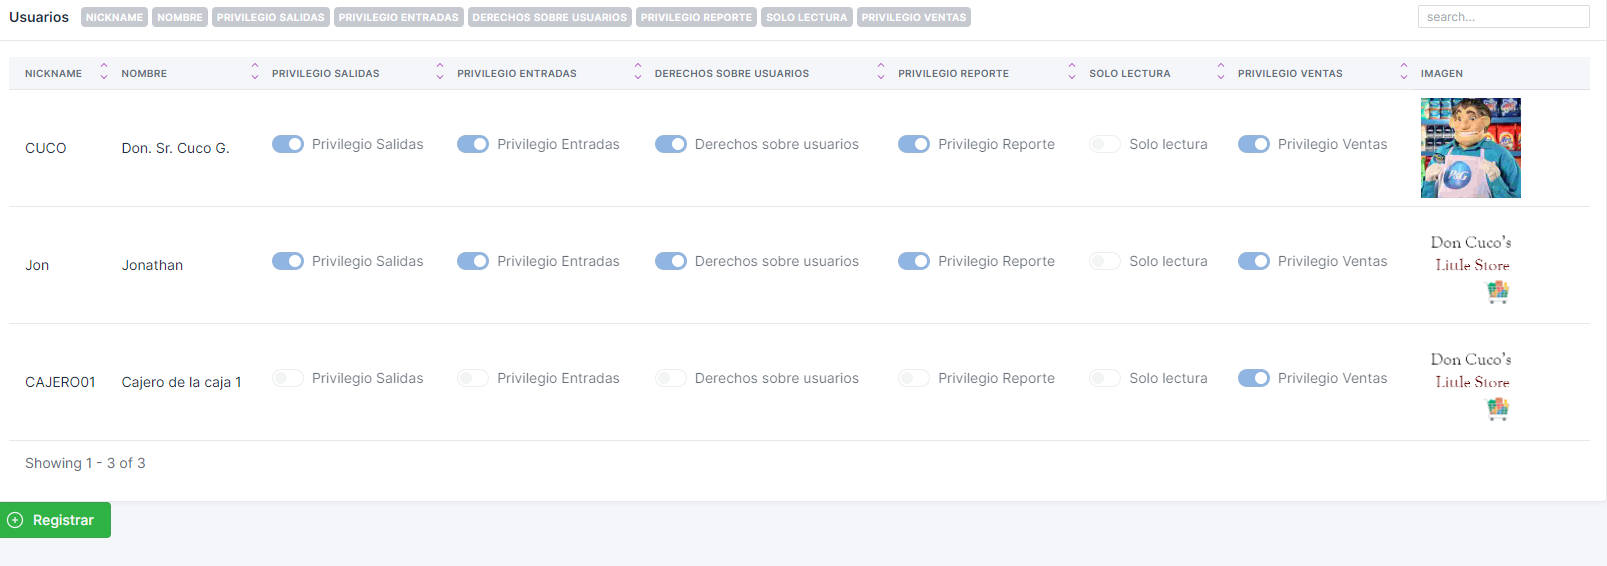
\includegraphics[scale=0.4]{USUARIOPS.PNG}\\
		\caption{Usuarios/Roles}
	\end{figure}

Aquí se podrá ver nuestos usuarios y que privilegios tendrán dentro de la aplicación, está vista solo será por el Administrador.\\



\subsection{Proveedores}

	\begin{figure}[!htb]
		\centering
		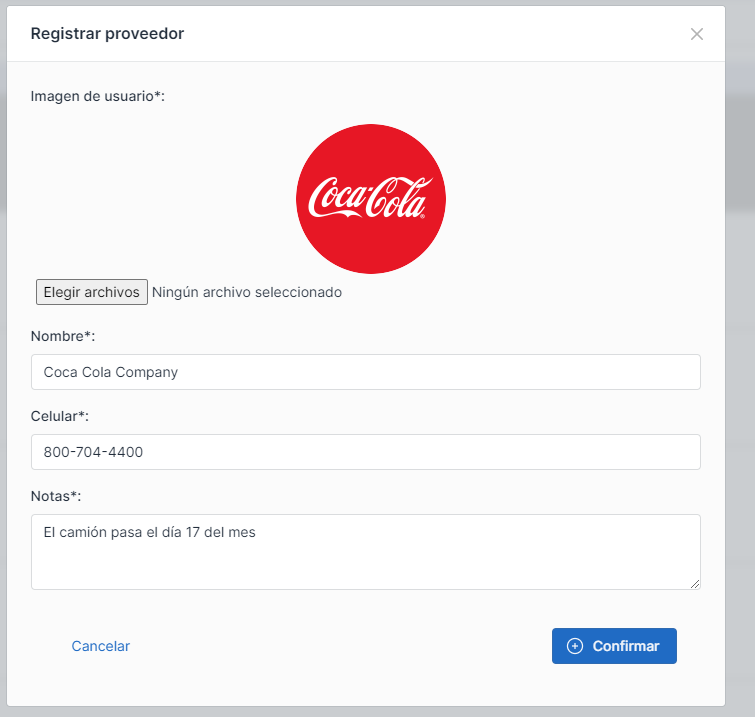
\includegraphics[scale=0.5]{ALTAPROVEEDOR.PNG}\\
		\caption{Venta para dar de Alta a nuestros Provedores}
	\end{figure}
		Cuenta con las siguientes opciones:
		\begin{itemize}
	\item Elegir archivos: Vista previa que tendremos para identificar con facilidar nuestro proveedor
	\item Nombre: Nombre de la empresa de nuestro provedor
	\item Celular: Tener el contacto de nuestro proveedor
	\item Cancelar: Cancelará la opción d edar de alta un producto
	\item Confirmar: Se creará la nueva categoría en nuestro sistema
	\end{itemize}
		\begin{figure}[!htb]
		\centering
		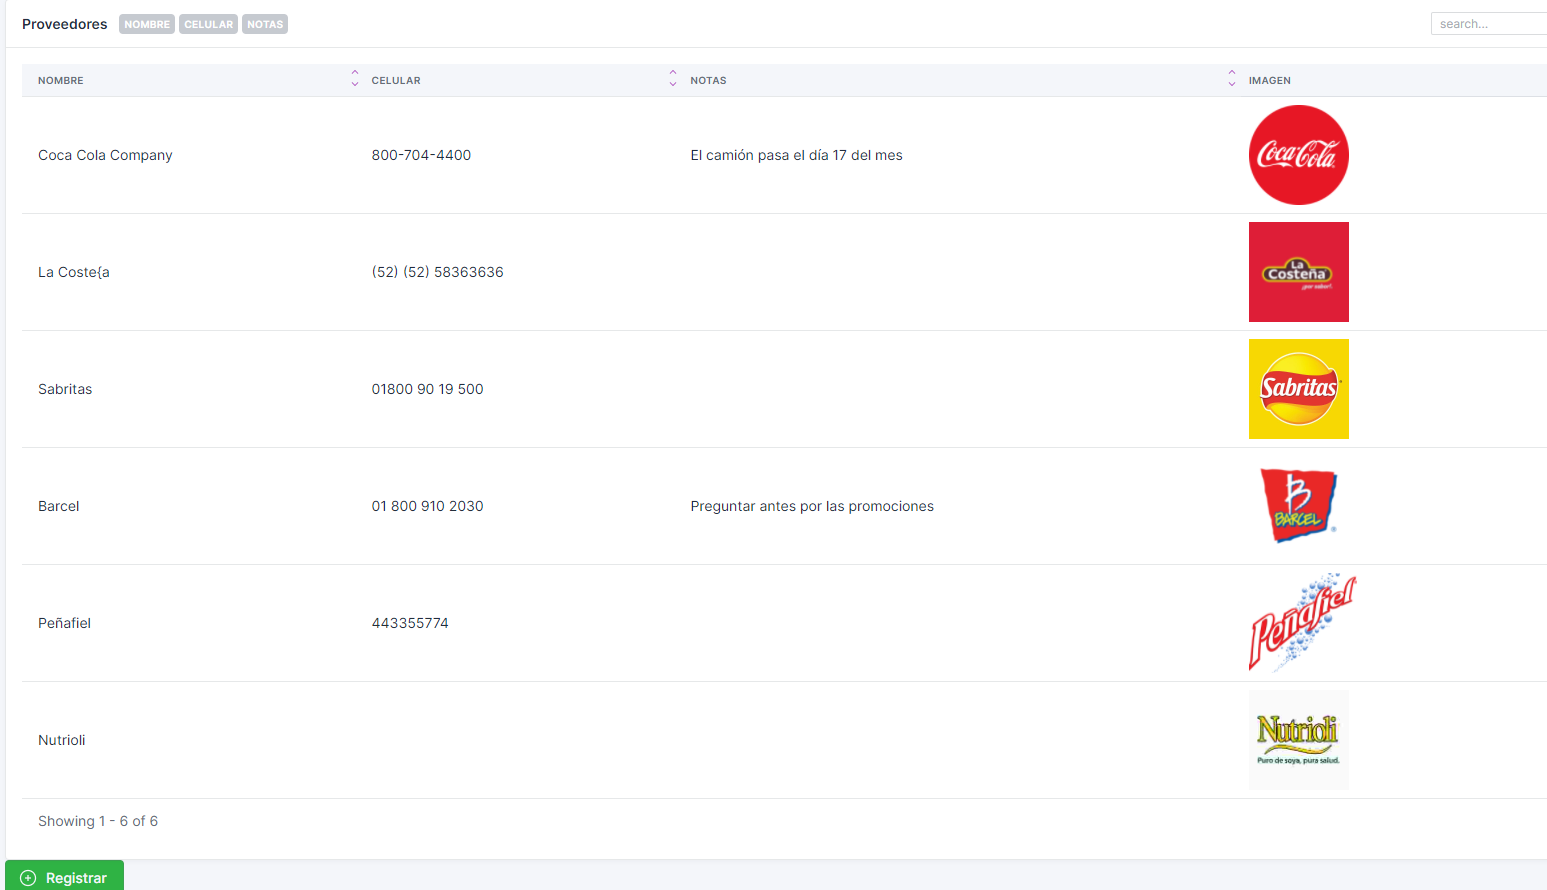
\includegraphics[scale=0.4]{PROVEEDORES.PNG}
		\caption{Vista de nuestra lista de proveedores}
	\end{figure}
	
	Vista rápida de nuestros proveedores con su respectivo número\\

\subsection{Compras}

	\begin{figure}[!htb]
		\centering
		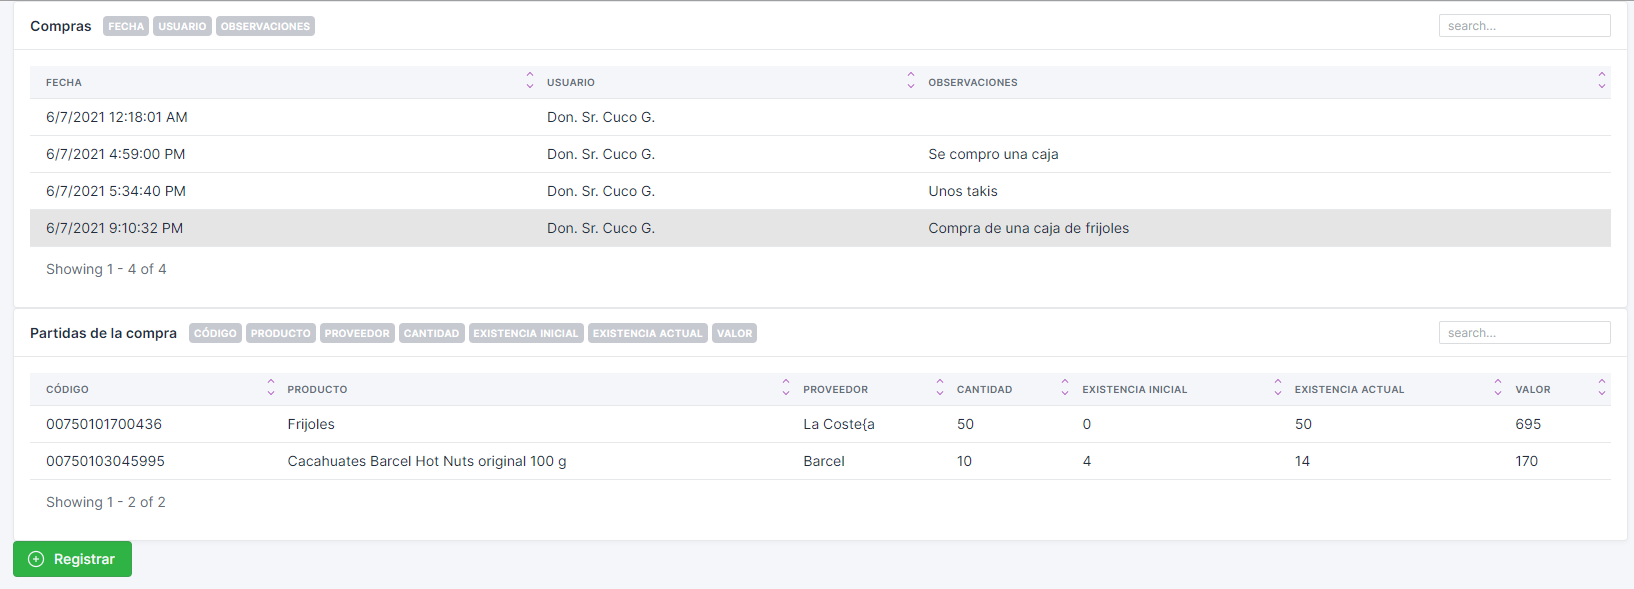
\includegraphics[scale=0.4]{COMPRAS.PNG}
		\caption{Vista de nuestras compras que se han realizado por nuestros usuarios}
	\end{figure}
	 En esta parte de la aplicación podemos tener mejor control de lo que saldrá de nuestra tienda y los gastos que se generarán.\\
		\begin{figure}[!htb]
		\centering
		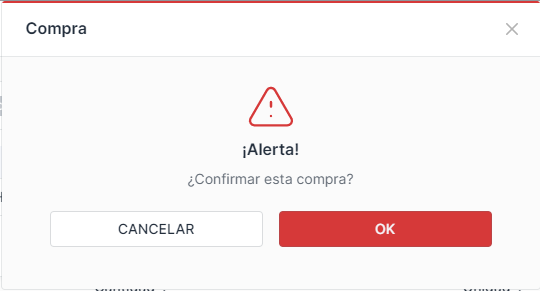
\includegraphics[scale=0.4]{CONFIRMAR.PNG}\\
		\caption{Ventana de alerta para confirmar nuestra compra}
	\end{figure}
	La ventana tiene los siguientes botones:\\
	\begin{itemize}
	
\item Cancelar: Cancelará la compra
\item Ok: Seguirá la compra
\item X: Cerrara la operación
\end{itemize}
	\begin{figure}[!htb]
		\centering
		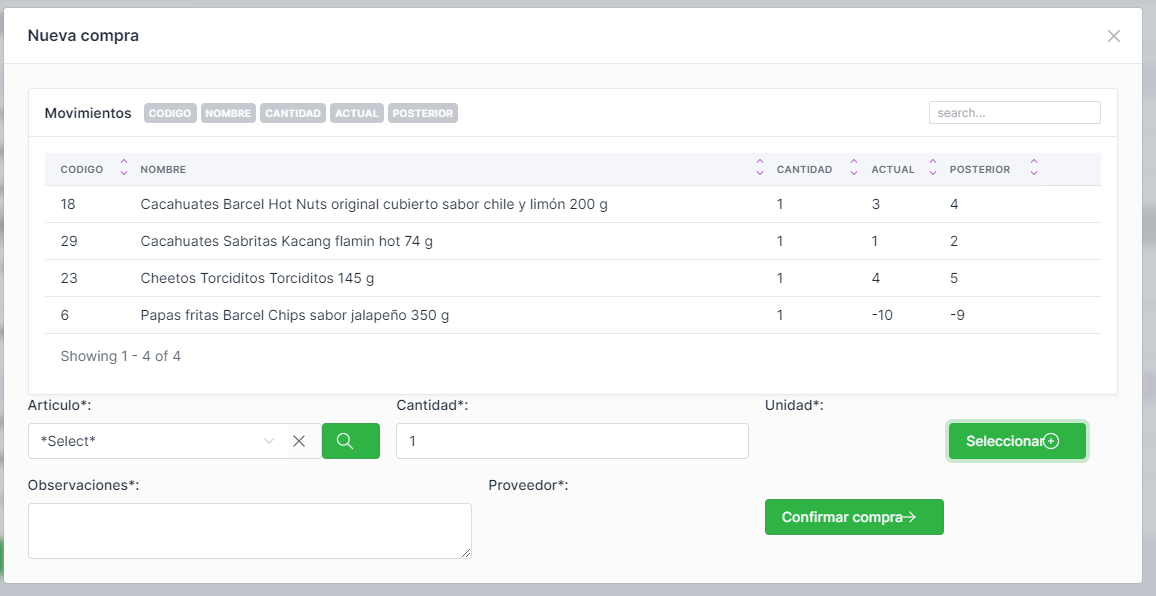
\includegraphics[scale=0.4]{NUEVACOMPRA.PNG}\\
		\caption{Ventana de nueva compra}
	\end{figure}
	\begin{figure}[!htb]
		\centering
		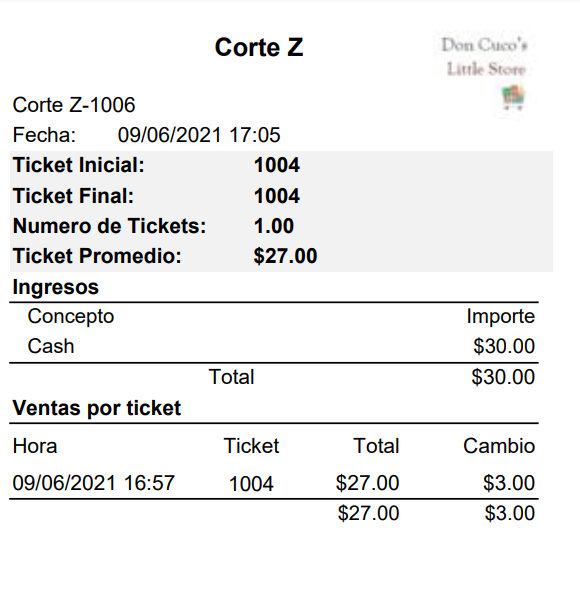
\includegraphics[scale=0.4]{CORTECAJA.PNG}
		\caption{Ticket de nuestra compra}
	\end{figure}
	
\clearpage

\subsection{Entrada/Salida}

	
		\begin{figure}[!htb]
		\centering
		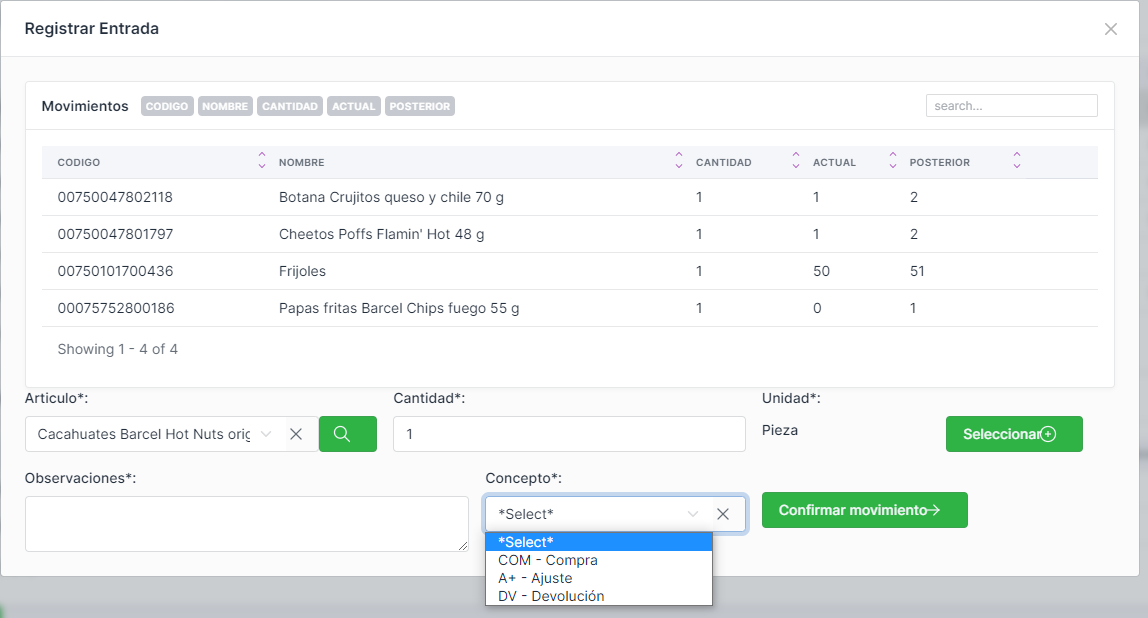
\includegraphics[scale=0.4]{ENTRADA.PNG}
		\caption{Entrada de nuestros productos}
	\end{figure}
Se tiene una ventana con los siguientes componentes: \\

\begin{enumerate}
	\item{\textbf{Cuadro de búsqueda:} Es un cuadro de búsqueda de productos, que permitirá realizar una búsqueda dentro de todo el inventario, remarcando y mostrando los que coindicen con la búsqueda, o mostrar un mensaje donde indique que no coincide ninguna búsqueda con lo ingresado.  }	
	\begin{itemize}
		\item{\textbf{Botón de Ordenar:} Es un filtro que permitirá ordenar los productos en el sistema, lo hará por todos los campos disponibles, id, alfabéticamente, según el nombre del proveedor. }
	\end{itemize}

	\item{\textbf{Campo de código:} Este campo permite tener una visualización de un identificador único a cada producto ingresado al inventario.}	
	\item{\textbf{Campo de texto:} Permitirá visualizar el nombre del producto, que se dio de alta en el inventario.}			
		
		
	\item{\textbf{Campo de texto:} Servirá para visualizar el número de los productos actuales en sistema.}	
	\item{\textbf{Campo de texto:} Servirá para visualizar el número posterior al movimiento de los productos actuales en sistema.}	
	
	\item{\textbf{Botón Cerrar:} Es el botón que cierra la ventana. Esta acción puede ser por medio de un botón o realizarse desde una equis (x) en el extremo superior derecho de la ventana actual.}	
\end{enumerate}
		\begin{figure}[h!]
		\centering
		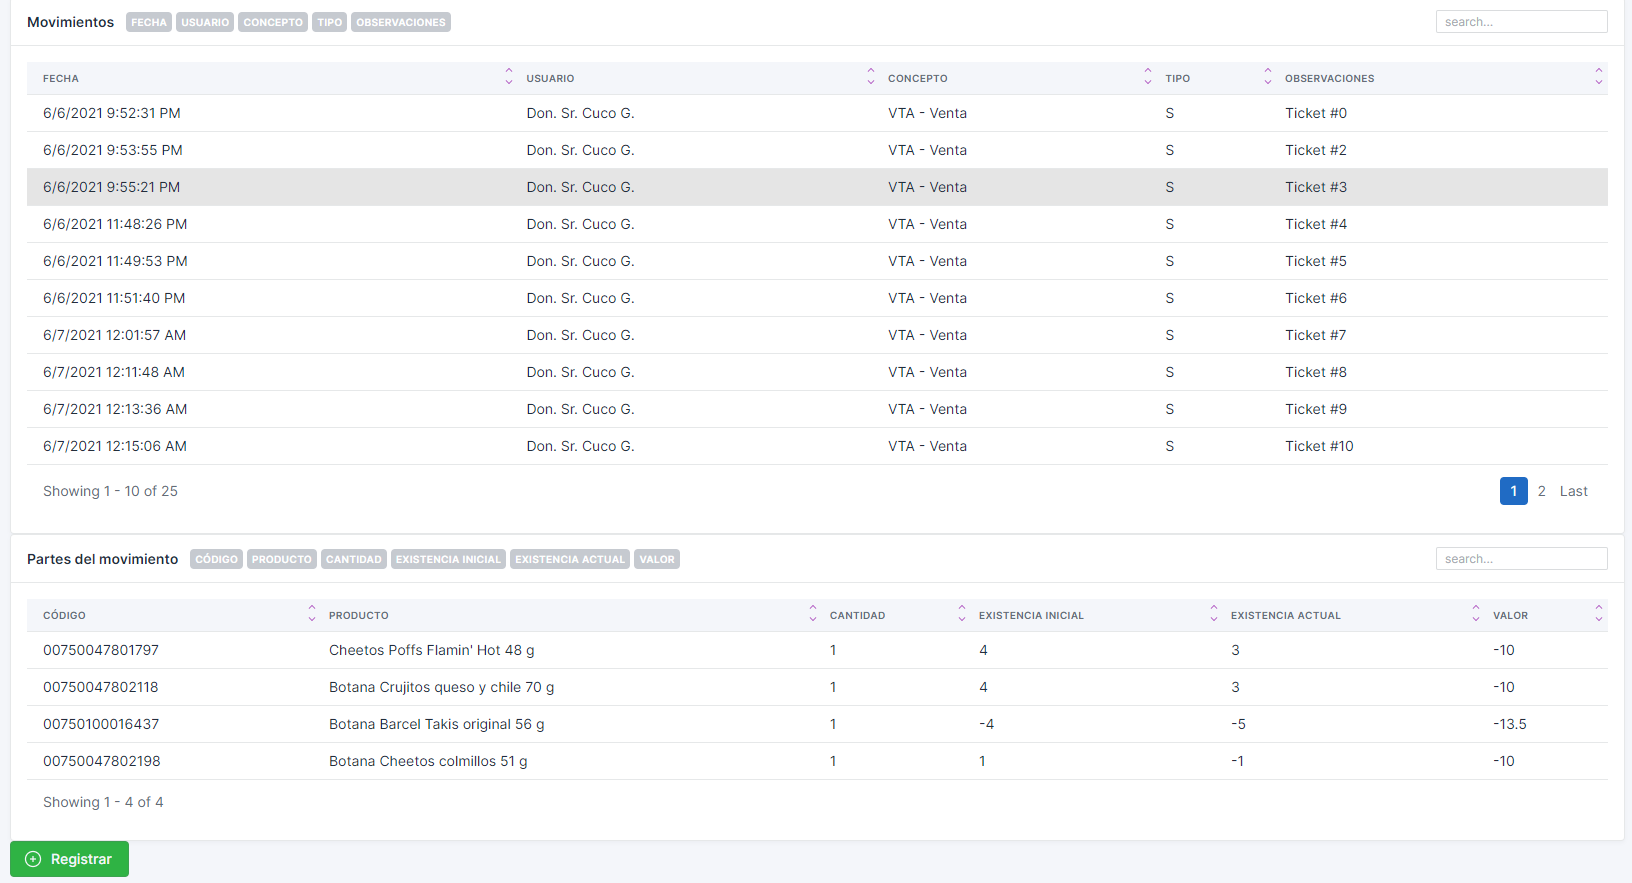
\includegraphics[scale=0.4]{SALIDAS.PNG}
		\caption{Salida de nuestros productos}
	\end{figure}
	Se tiene una ventana con los siguientes componentes: 

\begin{enumerate}
	\item{\textbf{Cuadro de búsqueda:} Es un cuadro de búsqueda de productos, que permitirá realizar una búsqueda dentro de todo el inventario, remarcando y mostrando los que coindicen con la búsqueda, o mostrar un mensaje donde indique que no coincide ninguna búsqueda con lo ingresado.  }	

	\item{\textbf{Campo de texto:} Permitirá visualizar el nombre del producto, que se dio de alta en el inventario.}			
    \item \textbf{Registrar:} Registrara una nueva salida del producto que seleccionemos 
	\item{\textbf{Botón Cerrar:} Es el botón que cierra la ventana. Esta acción puede ser por medio de un botón o realizarse desde una equis (x) en el extremo superior derecho de la ventana actual.}	
	\end{enumerate}
	
	\clearpage
	
\section{Reportes}

	\begin{figure}[h!]
		\centering
		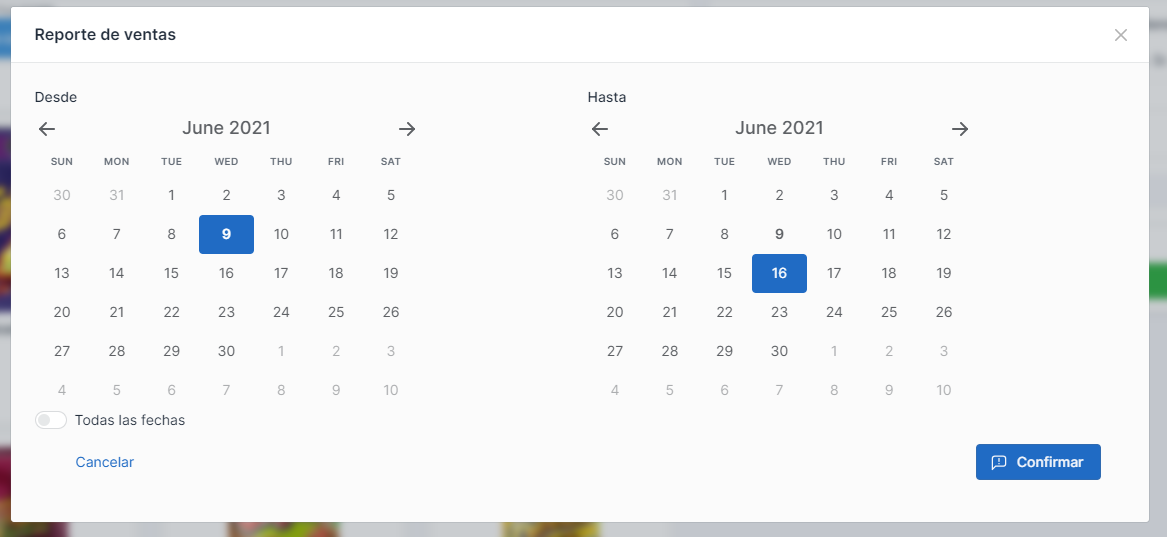
\includegraphics[scale=0.4]{FILTROREPORTES.PNG}
		\caption{Filtro de reportes}
	\end{figure}
	Esta ventana nos dará la opción de checar de que fecha a que fecha queremos ver los movimientos, la exitencia de nuestros productos y el reporte de ventas de nuestra tienda.\\
	
		\begin{figure}[h!]
		\centering
		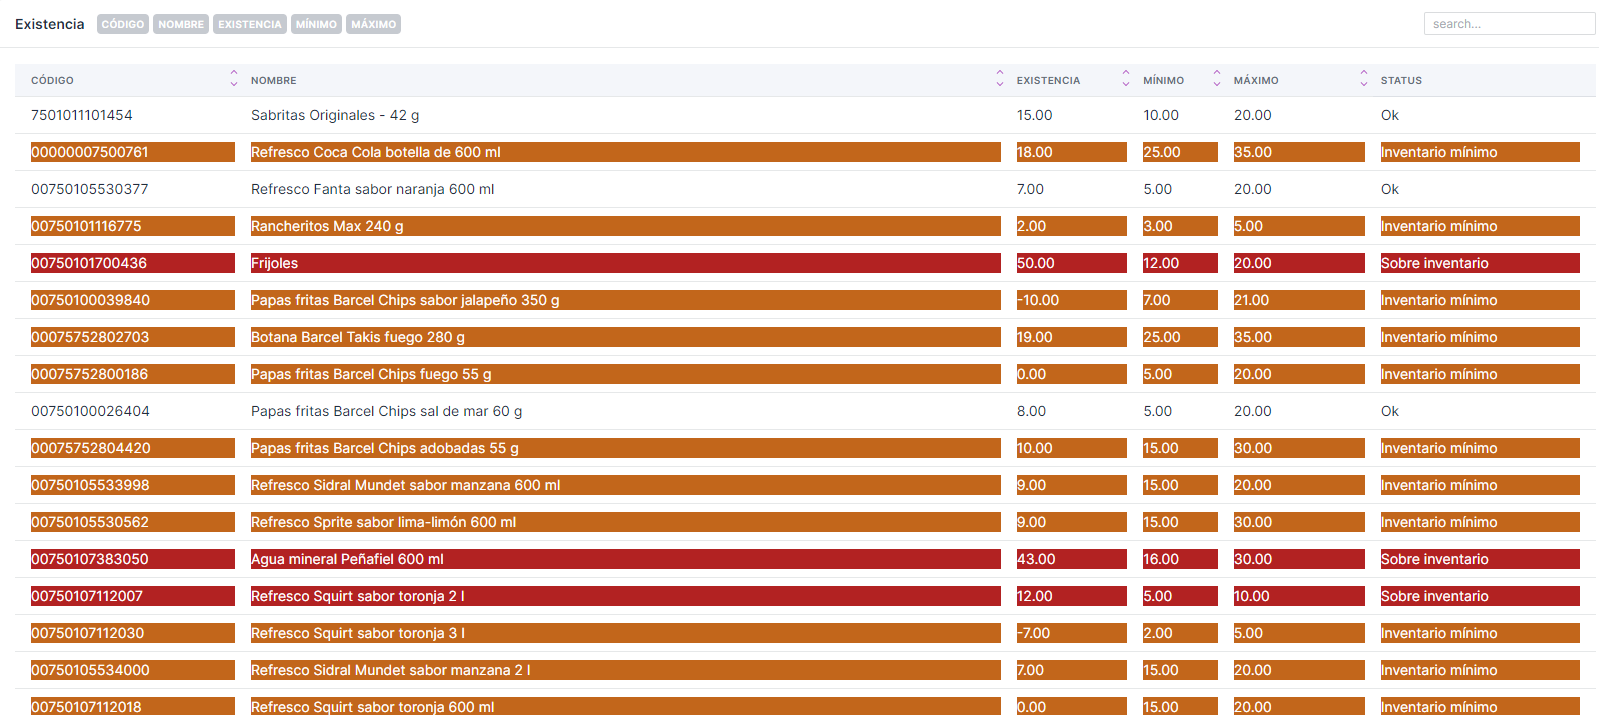
\includegraphics[scale=0.4]{REPORTEEXISTENCIA.PNG}\\
		\caption{Reporte de Existencia de nuestros productos}
	\end{figure}
	
		\begin{figure}[h!]
		\centering
		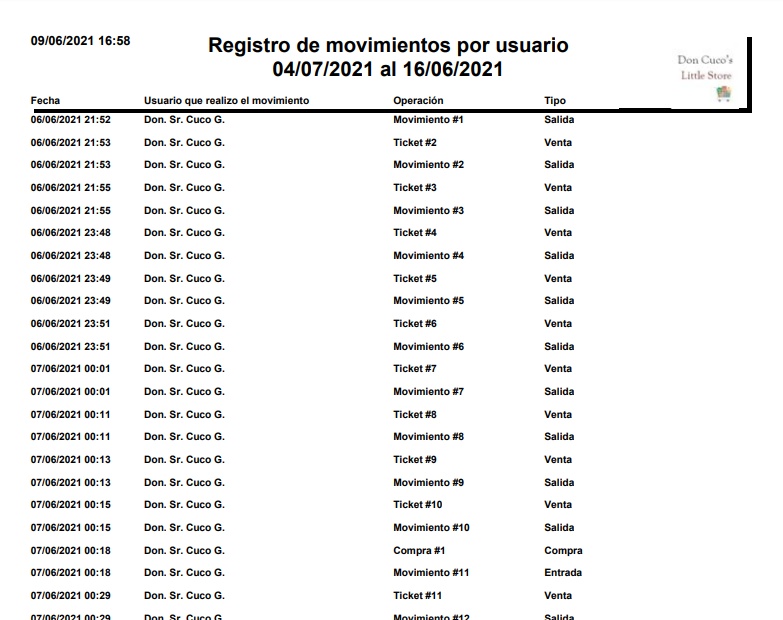
\includegraphics[scale=0.4]{REPORTEMOVIMIENTOS1.PNG}\\
		\caption{Reporte de movimientos de nuestros productos}
	\end{figure}
	
		\begin{figure}[h!]
		\centering
		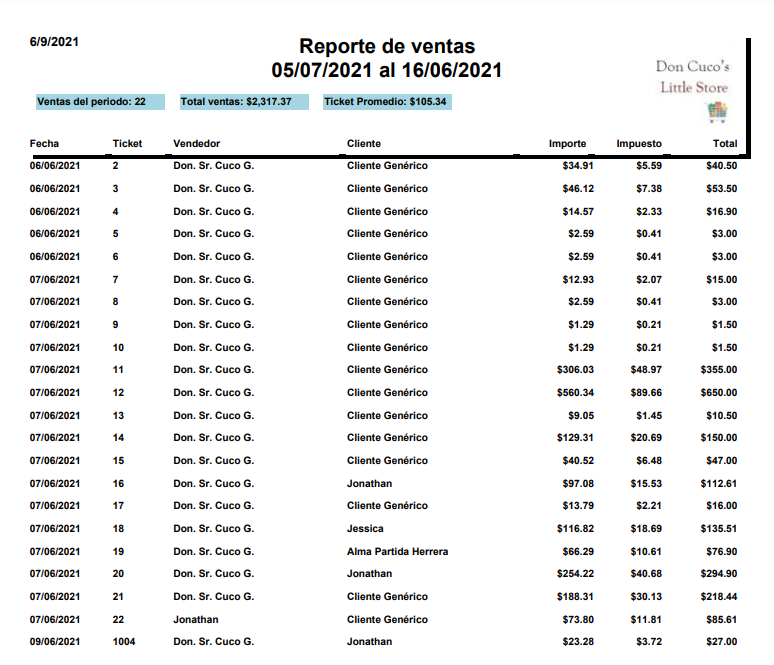
\includegraphics[scale=0.4]{REPORTEVENTAS.PNG}\\
		\caption{Reporte de Ventas de nuestros productos}
	\end{figure}
	
\clearpage

	\section{Movimientos}
		\begin{figure}[h!]
		\centering
		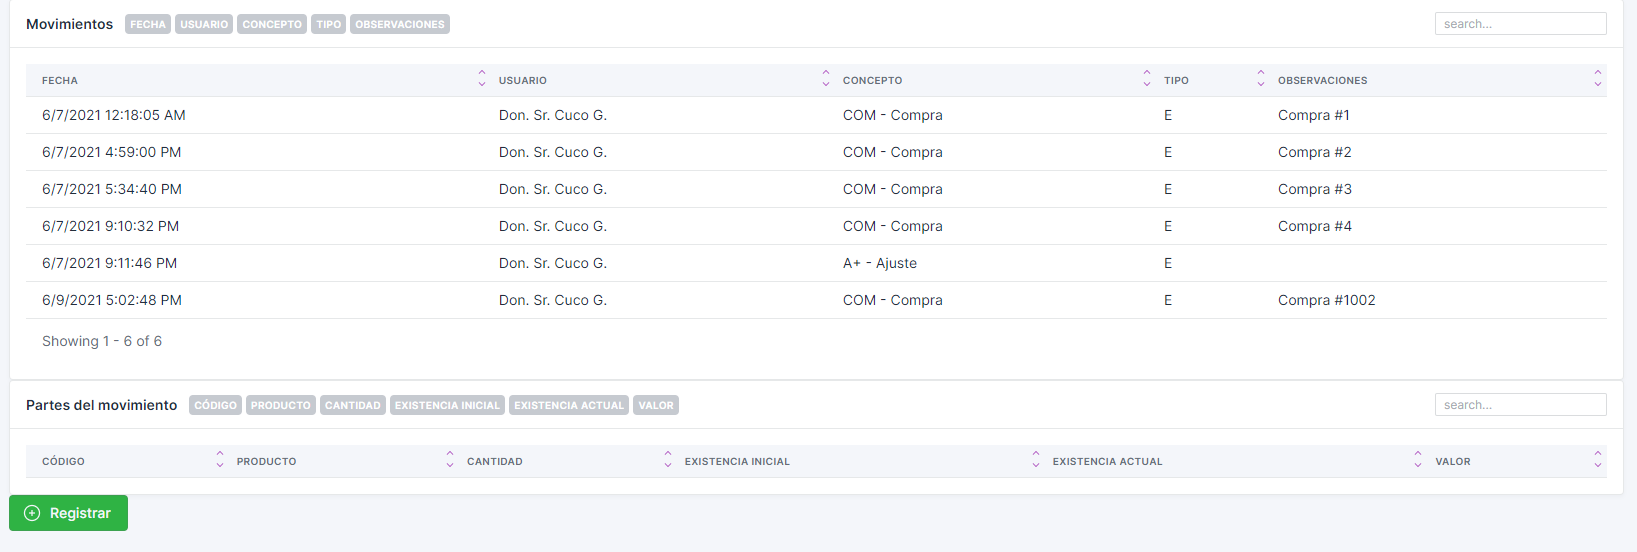
\includegraphics[scale=0.4]{MOVIMIENTOS1.PNG}
		\caption{Movimiento de existencia de productos}
	\end{figure}
	
	
	
		\begin{figure}[h!]
		\centering
		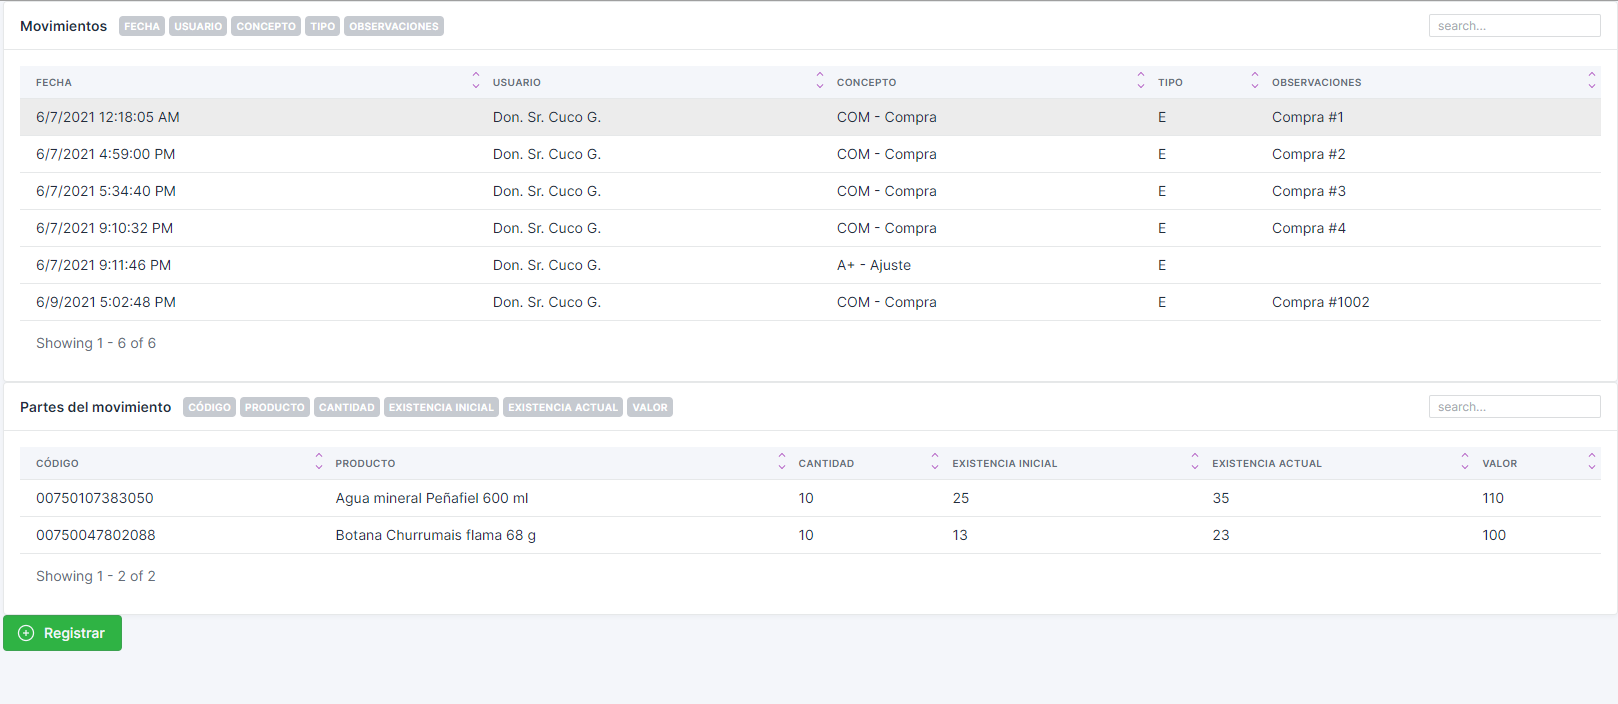
\includegraphics[scale=0.4]{MOVIMIENTOS2.PNG}
		\caption{Partes de los movimientos de productos}
		\end{figure}
		
		 En esta parte se visualizarán los movimientos relizados por el usuario, se verá quién hizo el ajuste o movimiento del productos y cuántos quedan en existencia actual e inicial.


%%%%%%%%%%%%%%% Manual Tecnico

 \section{Manual Técnico}
 \begin{figure}[!h]
     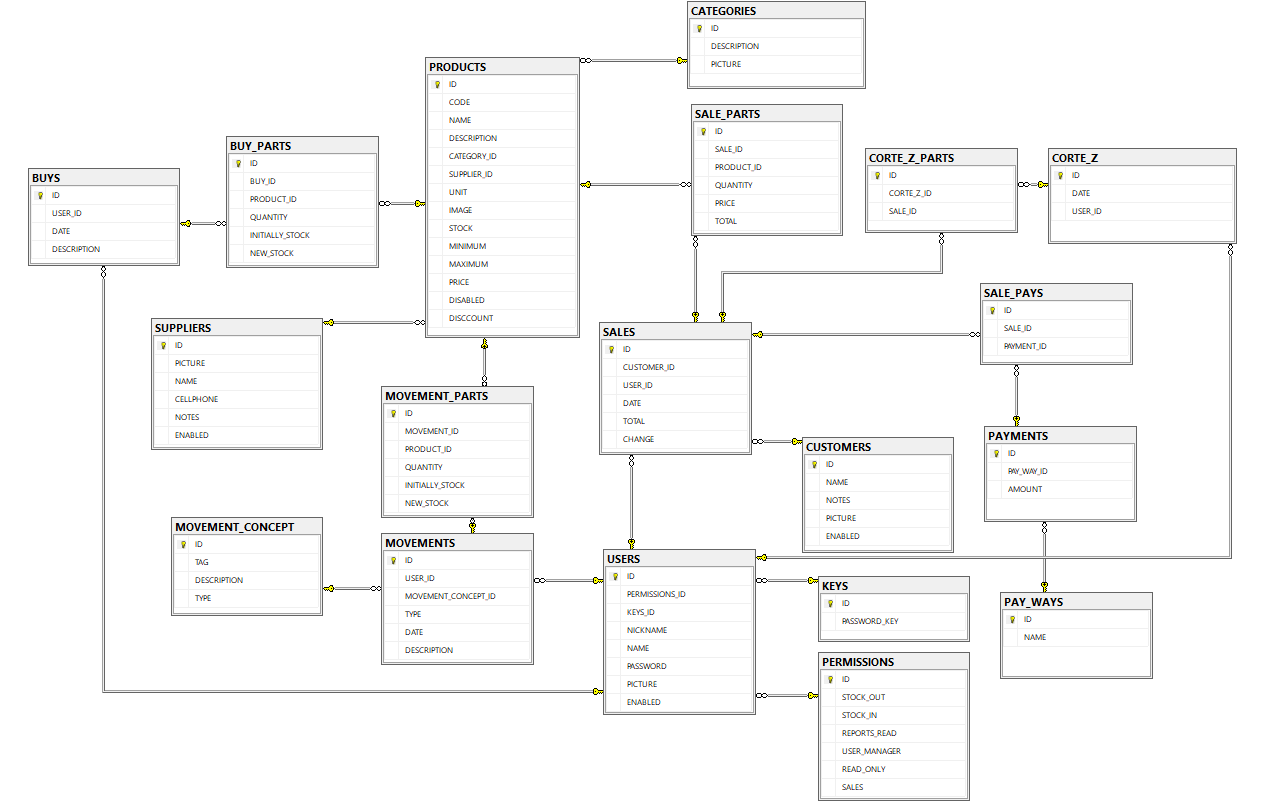
\includegraphics[width=16cm]{logico.png}\\
     \caption{Diseño lógico}
 \end{figure}
\begin{lstlisting}[language={SQL}]
    /* CREA UNA BASE DE DATOS EN BLANCO*/
    CREATE DATABASE DON_CUCO
    GO
    /* UTILIZA ESTA NUEVA BASE DE DATOS*/
    USE DON_CUCO
    GO
    ALMACENA LA INFORMACION SOBRE LAS CATEGORIAS DE PRODUCTOS\\
    CREATE TABLE CATEGORIES
    (
      ID INT PRIMARY KEY IDENTITY(1,1),
      DESCRIPTION VARCHAR(100) NOT NULL UNIQUE,
      PICTURE VARCHAR(MAX)
    );
    /*INFORMACION DE PROVEEDORES*/
    CREATE TABLE SUPPLIERS(
        ID INT PRIMARY KEY IDENTITY(1,1),
        PICTURE VARCHAR(MAX),
        NAME VARCHAR(100) NOT NULL,
        CELLPHONE VARCHAR(100),
        NOTES VARCHAR(MAX),
        ENABLED BIT NOT NULL DEFAULT 0
    
    );
    /*INFORMACION DE PRODUCTOS*/
    CREATE TABLE PRODUCTS(
        ID INT PRIMARY KEY IDENTITY(1,1),
        CODE VARCHAR(100) UNIQUE NOT NULL,
        NAME VARCHAR(100) NOT NULL,
        DESCRIPTION VARCHAR(MAX),
        CATEGORY_ID INT FOREIGN KEY REFERENCES CATEGORIES NOT NULL,
        SUPPLIER_ID INT FOREIGN KEY REFERENCES SUPPLIERS NOT NULL,
        UNIT VARCHAR(100) NOT NULL,
        IMAGE VARCHAR(MAX),
        STOCK REAL NOT NULL DEFAULT 0,
        MINIMUM REAL NOT NULL DEFAULT 0,
        MAXIMUM REAL NOT NULL DEFAULT 0,
        PRICE REAL NOT NULL DEFAULT 0,
        DISABLED BIT NOT NULL DEFAULT 0,
        DISCCOUNT INTEGER NOT NULL DEFAULT 0
    );
    /*INFORMACION/MATRIZ DE PERMISOS DE USUARIO*/
    CREATE TABLE PERMISSIONS
    (
        ID INT PRIMARY KEY IDENTITY (1,1),
        STOCK_OUT BIT DEFAULT 0,
        STOCK_IN BIT DEFAULT 0,
        REPORTS_READ BIT DEFAULT 0,
        USER_MANAGER BIT DEFAULT 0,
        READ_ONLY BIT DEFAULT 0,
        SALES BIT DEFAULT 0,
    );
    /* LLAVES,TOKENS DE SEGURIDAD PARA DESENCRIPTAR PASSWORDS DE USUARIO*/
    CREATE TABLE KEYS(
        ID INT PRIMARY KEY IDENTITY(1,1),
        PASSWORD_KEY VARCHAR(37) DEFAULT NEWID()
    );
    /*INFORMACION SOBRE USUARIOS DEL SITEMA */
    CREATE TABLE USERS(
        ID INT PRIMARY KEY IDENTITY(1,1),
        PERMISSIONS_ID INT FOREIGN KEY REFERENCES PERMISSIONS NOT NULL,
        KEYS_ID INT FOREIGN KEY REFERENCES KEYS NOT NULL,
        NICKNAME VARCHAR(100) NOT NULL UNIQUE,
        NAME VARCHAR(100) NOT NULL,
        PASSWORD VARBINARY(MAX) NOT NULL,
        PICTURE VARCHAR(MAX) DEFAULT NULL,
        ENABLED BIT NOT NULL DEFAULT 0
    );
    /*LISTADO DE CONCEPTOS DE MOVIMIENTOS*/
    CREATE TABLE MOVEMENT_CONCEPT
    (
        ID INT PRIMARY KEY IDENTITY(1,1),
        TAG VARCHAR(10) NOT NULL,
        DESCRIPTION VARCHAR(100),
        TYPE VARCHAR(1)
    );
    /*CABECERA DE LA COMPRA*/
    CREATE TABLE BUYS( --1 para que te de el id de movement
        ID INT PRIMARY KEY IDENTITY(1,1),
        USER_ID INT FOREIGN KEY REFERENCES USERS NOT NULL,
        DATE DATETIME NOT NULL DEFAULT GETDATE(),
        DESCRIPTION VARCHAR(100)
    );
    /*PARTIDAS DE LA COMPRA*/
    CREATE TABLE BUY_PARTS(  
        ID INT PRIMARY KEY IDENTITY(1,1),
        BUY_ID INT FOREIGN KEY REFERENCES BUYS NOT NULL,
        PRODUCT_ID INT FOREIGN KEY REFERENCES PRODUCTS NOT NULL,
        QUANTITY REAL NOT NULL DEFAULT 0,
        INITIALLY_STOCK REAL NOT NULL,
        NEW_STOCK REAL NOT NULL
    );
    /*CABECERA DE EL MOVIMIENTO (E/S)*/
    CREATE TABLE MOVEMENTS( --1 para que te de el id de movement
        ID INT PRIMARY KEY IDENTITY(1,1),
        USER_ID INT FOREIGN KEY REFERENCES USERS NOT NULL,
        MOVEMENT_CONCEPT_ID INT FOREIGN KEY REFERENCES MOVEMENT_CONCEPT NOT NULL,
        TYPE VARCHAR(1) NOT NULL,
        DATE DATETIME NOT NULL DEFAULT GETDATE(),
        DESCRIPTION VARCHAR(100)
    );
    /*PARTIDAS DEL MOVIMIENTO*/
    CREATE TABLE MOVEMENT_PARTS(  
        ID INT PRIMARY KEY IDENTITY(1,1),
        MOVEMENT_ID INT FOREIGN KEY REFERENCES MOVEMENTS NOT NULL,
        PRODUCT_ID INT FOREIGN KEY REFERENCES PRODUCTS NOT NULL,
        QUANTITY REAL NOT NULL DEFAULT 0,
        INITIALLY_STOCK REAL NOT NULL,
        NEW_STOCK REAL NOT NULL
    );
    /*REGISTRO DE CLIENTES*/
    CREATE TABLE CUSTOMERS(
        ID INT PRIMARY KEY IDENTITY(1,1),
        NAME VARCHAR(100) NOT NULL,
        NOTES VARCHAR(MAX),
        PICTURE VARCHAR(MAX),
        ENABLED BIT NOT NULL DEFAULT 0
    );
    /*LISTADO DE LAS FORMAS DE PAGO DISPONIBLES*/
    CREATE TABLE PAY_WAYS(	
        ID INT PRIMARY KEY IDENTITY(1,1),
        NAME VARCHAR(50)
    );
    /*LISTADO DE PAGOS RECIBIDOS */
    CREATE TABLE PAYMENTS
    (
        ID INT PRIMARY KEY IDENTITY(1,1),
        PAY_WAY_ID INT FOREIGN KEY REFERENCES PAY_WAYS,
        AMOUNT FLOAT NOT NULL DEFAULT 0
    );
    /*CABECERA DE UNA VENTA*/
    CREATE TABLE SALES(
        ID INT PRIMARY KEY IDENTITY(1,1),
        CUSTOMER_ID INT FOREIGN KEY REFERENCES CUSTOMERS NOT NULL,
        USER_ID INT FOREIGN KEY REFERENCES USERS NOT NULL,
        DATE DATETIME DEFAULT GETDATE(),
        TOTAL REAL,
        CHANGE REAL
    );
    /*PARTIDAS DE UNA VENTA*/
    CREATE TABLE SALE_PARTS(
        ID INT PRIMARY KEY IDENTITY(1,1),
        SALE_ID INT FOREIGN KEY REFERENCES SALES NOT NULL,
        PRODUCT_ID INT FOREIGN KEY REFERENCES PRODUCTS NOT NULL,
        QUANTITY REAL,
        PRICE REAL,
        TOTAL REAL
    );
    /*PAGOS REALIZADOS EN UNA VENTA ESPECIFICA*/
    CREATE TABLE SALE_PAYS(
        ID INT PRIMARY KEY IDENTITY(1,1),
        SALE_ID INT FOREIGN KEY REFERENCES SALES NOT NULL,
        PAYMENT_ID INT FOREIGN KEY REFERENCES PAYMENTS
    );
    GO
    /*REGISTRO DE CORTE DE CAJA DE CIERRE*/
    CREATE TABLE CORTE_Z(
        ID INT PRIMARY KEY IDENTITY(1,1),
        DATE DATETIME,
        USER_ID INT FOREIGN KEY REFERENCES USERS NOT NULL);
    GO
    /*LISTADO DE VENTAS POR CORTE DE CAJA*/
    CREATE TABLE CORTE_Z_PARTS(
        ID INT PRIMARY KEY IDENTITY(1,1),
        CORTE_Z_ID INT FOREIGN KEY REFERENCES CORTE_Z NOT NULL,
        SALE_ID INT FOREIGN KEY REFERENCES SALES NOT NULL,
    );
    GO
    /*REALIZA UN NUEVO CORTE DE CAJA, INSERTA LA LLAVE DE LAS VENTAS QUE PARTICIPAN EN ESTE CORTE*/
    CREATE PROCEDURE SP_CORTE_Z(@USER_ID INT)
    AS
    BEGIN
        DECLARE @CORTE_Z_ID INT
        INSERT INTO CORTE_Z(DATE,USER_ID) VALUES(GETDATE(),@USER_ID);
        SELECT @CORTE_Z_ID=SCOPE_IDENTITY();
        INSERT INTO CORTE_Z_PARTS(CORTE_Z_ID,SALE_ID) SELECT @CORTE_Z_ID,ID FROM SALES WHERE NOT EXISTS 
        (SELECT ID FROM CORTE_Z_PARTS CZ WHERE CZ.SALE_ID=SALES.ID)
        SELECT @CORTE_Z_ID
    END;
    GO
    /*RETORNA UNA VISTA DE LAS VENTAS QUE AUN NO ESTAN AGRUPADAS EN ALGUN CORTE DE CAJA*/
    CREATE VIEW VIEW_GETCORTEZ_SALES
    AS
    select SALES.ID,SALES.DATE as 'Fecha',SALES.TOTAL,
    SALES.CHANGE,USERS.NAME as 'User',CUSTOMERS.NAME as 'Customers' 
    From sales
    inner join USERS ON USERS.ID=SALES.USER_ID
    inner join CUSTOMERS ON CUSTOMERS.ID=SALES.CUSTOMER_ID
    WHERE NOT EXISTS 
    (SELECT ID FROM CORTE_Z_PARTS CZ WHERE CZ.SALE_ID=SALES.ID)
    GO
    /*RETORNA UN LISTADO DE LOS PRODUCTOS DE LAS VENTAS QUE AUN NO ESTAN AGRUPADAS EN ALGUN CORTE DE CAJA*/
    CREATE VIEW VIEW_GETCORTEZ_PRODUCTS
    AS
    select SALE_ID,NAME,QUANTITY,SALE_PARTS.PRICE,
    TOTAL/1.16 AS 'IMPUESTO',
    TOTAL-TOTAL/1.16 AS 'IMPORTE',
    TOTAL
    From SALE_PARTS
    INNER JOIN PRODUCTS ON PRODUCTS.ID=SALE_PARTS.PRODUCT_ID
    WHERE NOT EXISTS 
    (SELECT ID FROM CORTE_Z_PARTS CZ WHERE CZ.SALE_ID=SALE_PARTS.SALE_ID)
    GO
    /*RETORNA UN LISTADO DE TODOS LOS PAGOS QUE SE HICIERON EN LAS VENTAS QUE AUN NO ESTAN AGRUPADAS EN ALGUN CORTE DE CAJA*/
    CREATE VIEW VIEW_PAYMENTS_CORTE_Z
    AS
    select SALE_ID,NAME,AMOUNT
    From SALE_PAYS
    INNER JOIN PAYMENTS ON PAYMENTS.ID=SALE_PAYS.PAYMENT_ID
    INNER JOIN PAY_WAYS ON PAY_WAYS.ID=PAYMENTS.PAY_WAY_ID
    WHERE NOT EXISTS 
    (SELECT ID FROM CORTE_Z_PARTS CZ WHERE CZ.SALE_ID=SALE_PAYS.SALE_ID)
    GO
    /*INSERTA LA CABECERA DE UNA VENTA NUEVA Y RETORNA SU ID*/
    CREATE PROCEDURE SP_SAVE_SALE (@CUSTOMER_ID INT ,@USER_ID INT,@TOTAL FLOAT,@CHANGE FLOAT)
    AS
    BEGIN
    INSERT INTO SALES(CUSTOMER_ID,USER_ID,DATE,TOTAL,CHANGE) VALUES (@CUSTOMER_ID,@USER_ID,GETDATE(),@TOTAL,@CHANGE);
    SELECT SCOPE_IDENTITY();
    END
    GO
    /*INSERTA UNA PARTIDA DE UNA VENTA NUEVA Y RETORNA SU ID*/
    CREATE PROCEDURE SP_SAVE_SALE_PART
    (@SALE_ID INT ,@PRODUCT_ID INT,@PRICE FLOAT,@QUANTITY FLOAT,@TOTAL FLOAT)
    AS
    BEGIN
    --UPDATE PRODUCTS SET STOCK-=@QUANTITY WHERE ID=@PRODUCT_ID 
    INSERT INTO SALE_PARTS
    (SALE_ID,PRODUCT_ID,QUANTITY,PRICE,TOTAL) 
    VALUES (@SALE_ID,@PRODUCT_ID,@QUANTITY,@PRICE,@TOTAL);
    SELECT SCOPE_IDENTITY();
    END
    GO
    /*INSERTA LOS MÉTODOS DE PAGO DE UNA VENTA NUEVA*/
    CREATE PROCEDURE SP_SAVE_SALE_PAYS(@SALE_ID INT,@PAYMENT_ID FLOAT)
    AS
    BEGIN
    INSERT INTO SALE_PAYS(SALE_ID,PAYMENT_ID) VALUES (@SALE_ID,@PAYMENT_ID);
    END
    GO
    /*INSERTA LA CANTIDAD EN DINERO DE UN MÉTODO DE PAGO DE UNA VENTA NUEVA*/
    CREATE PROCEDURE SP_SAVE_PAYMENT(@PAY_WAY_ID INT,@AMOUNT FLOAT)
    AS
    BEGIN
    INSERT INTO PAYMENTS(PAY_WAY_ID,AMOUNT) VALUES (@PAY_WAY_ID,@AMOUNT);
    SELECT SCOPE_IDENTITY();
    END
    GO
    --INSERTA LOS TIPOS DE PAGO POR DEFECTO
    INSERT INTO PAY_WAYS (NAME) VALUES('Cash');
    INSERT INTO PAY_WAYS (NAME) VALUES('Vale');
    INSERT INTO PAY_WAYS (NAME) VALUES('Card');
    --Loguea al usuario pidiendo como parametros Nickname y Password y desencriptando a su vez la contraseña para validarla 
    GO
    CREATE PROCEDURE SP_LOGIN (@NICKNAME VARCHAR(100), @PASSWORD NVARCHAR(50))
    AS
    BEGIN
            DECLARE @USER_ID INT;
            SELECT @USER_ID=ID FROM USERS WHERE NICKNAME=@NICKNAME
            IF(@USER_ID>0)
                BEGIN
                  DECLARE @PASSWORD_KEY VARCHAR(37);
                  DECLARE @REAL_PASSWORD VARCHAR(50);
                  DECLARE @KEY_ID INT;
                  SELECT @KEY_ID=KEYS_ID FROM USERS WHERE ID=@USER_ID
    
                  SELECT @PASSWORD_KEY=PASSWORD_KEY FROM KEYS WHERE ID=@KEY_ID
                  
                  SELECT @REAL_PASSWORD=CONVERT(NVARCHAR(MAX), DECRYPTBYPASSPHRASE(@PASSWORD_KEY, PASSWORD)) FROM USERS WHERE ID=@USER_ID
                  IF (@REAL_PASSWORD=@PASSWORD)
                  BEGIN
                    SELECT 1 AS 'LOGIN_STATUS';
                    RETURN;
                  END
                END
                SELECT 0 AS 'LOGIN_STATUS';
        END;
    GO
    --Registra y/o Actualiza al usuario pidiendo como parametros nickname,contraseña,Nobre y una imagen. 
    --- Encripta la contraseña por seguridad del ususario
    CREATE PROCEDURE SP_REGISTER(@NICKNAME VARCHAR(100), @PASSWORD NVARCHAR(50),@NAME VARCHAR(100),@PICTURE VARCHAR(MAX),@ENABLED BIT,@ID INT)
    AS
    BEGIN
        IF(@ID<=0)
        BEGIN
        DECLARE @PERMISSIONS_ID INT;
        DECLARE @KEY_ID INT;
        DECLARE @KEY VARCHAR(MAX);
        DECLARE @ENCRYPTED_PASSWORD VARBINARY(MAX);
    
        INSERT INTO PERMISSIONS DEFAULT VALUES
        SELECT @PERMISSIONS_ID=SCOPE_IDENTITY();
    
        INSERT INTO KEYS DEFAULT VALUES
        SELECT @KEY_ID=SCOPE_IDENTITY();
        SELECT @KEY =PASSWORD_KEY FROM KEYS WHERE ID=@KEY_ID
    
        SELECT @ENCRYPTED_PASSWORD = ENCRYPTBYPASSPHRASE(@KEY, @PASSWORD);
            
        INSERT INTO USERS(PERMISSIONS_ID,KEYS_ID,NICKNAME,NAME,PASSWORD,PICTURE,ENABLED)
        VALUES(@PERMISSIONS_ID,@KEY_ID,@NICKNAME,@NAME,@ENCRYPTED_PASSWORD,@PICTURE,@ENABLED)
        END ELSE
        BEGIN
    
        SELECT @KEY_ID=KEYS_ID FROM USERS WHERE ID=@ID
        SELECT @KEY =PASSWORD_KEY FROM KEYS WHERE ID=@KEY_ID
        SELECT @ENCRYPTED_PASSWORD = ENCRYPTBYPASSPHRASE(@KEY, @PASSWORD);
        UPDATE USERS SET NICKNAME=@NICKNAME,NAME=@NAME,PASSWORD=@ENCRYPTED_PASSWORD,PICTURE=@PICTURE,ENABLED=@ENABLED
        WHERE ID=@ID
    
        END
    END;
    GO
    
    -------PRODUCTS--------
    GO
    --Obtiene la existencia de un producto mendante su Id
    CREATE PROCEDURE SP_GETSTOCK(@ID INT)
    AS
    BEGIN
    SELECT STOCK FROM PRODUCTS WHERE ID=@ID
    END;
    GO
    ---Obtiene los productos donde DISABLED sea igual a cero y ordnandolos por su nombre
    CREATE PROCEDURE SP_GET_PRODUCTS
    AS
    BEGIN
        SELECT * FROM PRODUCTS WHERE DISABLED=0 ORDER BY NAME
    END;
    GO
    ---Obtiene los productos por su codigo,donde DISABLED sea igual a cero y ordnandolos por su nombre
    CREATE PROCEDURE SP_FIND_PRODUCT(@CODE VARCHAR(100))
    AS
    BEGIN
        SELECT * FROM PRODUCTS WHERE DISABLED=0 AND CODE=@CODE ORDER BY NAME
    END;
    GO
    ---Obtiene todos los productos de la tabla Products
    CREATE PROCEDURE SP_GET_PRODUCT_BY_ID (@ID INT)
    AS
    BEGIN
        SELECT *FROM PRODUCTS WHERE ID=@ID
    END
    GO
    ---Procedure para la busqueda de un producto donde el patrón del codigo o del nombre coincida
    CREATE PROCEDURE SP_SEARCH_PRODUCT(@SEARCH VARCHAR(200))
    AS
    BEGIN
        SELECT * FROM PRODUCTS WHERE DISABLED=0 AND CODE LIKE '%'+@SEARCH+'%' OR NAME LIKE '%'+@SEARCH+'%' ORDER BY NAME
    END;
    GO
    ---Obtiene los productos de una categoria 
    CREATE PROCEDURE SP_GET_PRODUCTS_BY_CATEGORY(@CATEGORY_ID INT)
    AS
    BEGIN
    SELECT * FROM PRODUCTS WHERE DISABLED=0 AND CATEGORY_ID=@CATEGORY_ID ORDER BY NAME
    END;
    GO
    ---Obtiene los productos por la categoria buscada 
    CREATE PROCEDURE SP_GET_PRODUCTS_BY_CATEGORY_FIND(@CATEGORY_ID INT,@SEARCH VARCHAR(MAX))
    AS
    BEGIN
    SELECT * FROM PRODUCTS WHERE DISABLED=0 AND CATEGORY_ID=@CATEGORY_ID AND NAME LIKE '%'+@SEARCH+'%' ORDER BY NAME
    END;
    GO
    --Obtiene las categorias y las ordena por su descripcion
    CREATE PROCEDURE SP_GET_CATEGORIES
    AS
    BEGIN
        SELECT *FROM CATEGORIES order by DESCRIPTION
    END;
    GO
    --Busca las categorias donde el patrón de la descripción categoria o de la descripción del producto coincida ordenandolos por su descripción
    CREATE PROCEDURE SP_FIND_CATEGORIES (@SEARCH VARCHAR(MAX)) 
    AS
    BEGIN
        SELECT DISTINCT CATEGORIES.ID,CATEGORIES.DESCRIPTION FROM CATEGORIES 
        INNER JOIN PRODUCTS ON PRODUCTS.CATEGORY_ID=CATEGORIES.ID
        WHERE CATEGORIES.DESCRIPTION LIKE '%'+@SEARCH+'%' OR PRODUCTS.DESCRIPTION LIKE '%'+@SEARCH+'%' order by CATEGORIES.DESCRIPTION,CATEGORIES.ID
    END;
    GO
    ---Obtiene los categoria por la descripción 
    CREATE PROCEDURE SP_GET_CATEGORY_BY_NAME (@NAME VARCHAR(100))
    AS
    BEGIN
        SELECT *FROM CATEGORIES WHERE DESCRIPTION=@NAME
    END;
    GO
    ---Obtiene los categoria por el Id 
    CREATE PROCEDURE SP_GET_CATEGORY_BY_ID (@ID INT)
    AS
    BEGIN
        SELECT *FROM CATEGORIES WHERE ID=@ID
    END;
    GO
    ---Obtiene todos los provedores de la tabla SUPPLIERS
    CREATE PROCEDURE SP_GET_SUPPLIERS
    AS
    BEGIN
        SELECT *FROM SUPPLIERS
    END;
    GO
    ---Registra y actualizacion de productos con los paramentros de id en caso de actulizar,codigo,nombre,etc...
    CREATE PROCEDURE SP_ABC_PRODUCT (@ID INT,@CODE VARCHAR(100),@NAME VARCHAR(100),@DESCRIPTION VARCHAR(MAX),
    @CATEGORY_ID INT,@SUPPLIER_ID INT,@UNIT VARCHAR(100),@IMAGE VARCHAR(MAX),@STOCK REAL,@MINIMUM REAL,@MAXIMUM REAL,
    @PRICE REAL,@DISABLED BIT,@DISCCOUNT REAL)
    AS
    BEGIN
        IF(@ID<=0)
        BEGIN
            INSERT INTO PRODUCTS (CODE,NAME,DESCRIPTION,CATEGORY_ID,SUPPLIER_ID,UNIT,IMAGE,STOCK,MINIMUM,MAXIMUM,PRICE,DISABLED,DISCCOUNT)
            VALUES(@CODE,@NAME,@DESCRIPTION,@CATEGORY_ID,@SUPPLIER_ID,@UNIT,@IMAGE,@STOCK,@MINIMUM,@MAXIMUM,@PRICE,@DISABLED,@DISCCOUNT)
        END ELSE
        BEGIN
            UPDATE PRODUCTS SET CODE=@CODE,NAME=@NAME,DESCRIPTION=@DESCRIPTION,CATEGORY_ID=@CATEGORY_ID,
            SUPPLIER_ID=@SUPPLIER_ID,UNIT=@UNIT,IMAGE=@IMAGE,STOCK=@STOCK,MINIMUM=@MINIMUM,MAXIMUM=@MAXIMUM,PRICE=@PRICE,DISABLED=@DISABLED,DISCCOUNT=@DISCCOUNT
            WHERE ID=@ID
        END
    END;
    GO
    ---Registra y actualizacion de categosrias con los paramentros de id en caso de actulizar,descripción e imagen
    CREATE PROCEDURE SP_ABC_CATEGORY (@ID INT,@DESCRIPTION VARCHAR(100),@PICTURE VARCHAR(MAX))
    AS
    BEGIN
        IF(@ID<=0)
        BEGIN
            INSERT INTO CATEGORIES(DESCRIPTION,PICTURE) VALUES(@DESCRIPTION,@PICTURE) 
        END ELSE
        BEGIN
            UPDATE CATEGORIES SET DESCRIPTION=@DESCRIPTION,PICTURE=@PICTURE WHERE ID=@ID
        END
    END;
    GO
    ------ALERTS-------
    CREATE VIEW VIEW_OVERSTOCKED
    AS
    SELECT * FROM PRODUCTS WHERE STOCK>=MAXIMUM;
    GO
    CREATE VIEW VIEW_UNDERSTOCKED
    AS
    SELECT * FROM PRODUCTS WHERE STOCK<=MINIMUM;
    GO
    CREATE VIEW VIEW_ALL_ALERTS
    AS
    SELECT * FROM PRODUCTS WHERE STOCK >= MAXIMUM OR STOCK <= MINIMUM;
    GO
    -----MOVEMENTS-----
    GO
    ---Obtiene todos las compras de la tabla BUYS mediante su Id
    CREATE PROCEDURE SP_GET_BUY_BY_ID(@ID INT)
    AS
    BEGIN
    SELECT * FROM BUYS WHERE ID =@ID;
    END;
    GO
    ---Obtiene todos los movimientos de la tabla MOVEMENTS
    CREATE PROCEDURE SP_GET_MOVEMENT(@ID INT)
    AS
    BEGIN
    SELECT * FROM MOVEMENTS WHERE ID =@ID;
    END;
    GO
    ---Obtiene todos las partes de los movimientos de la tabla MOVEMENT_PARTS
    CREATE PROCEDURE SP_GET_MOVEMENTPART_BY_ID(@ID INT)
    AS
    BEGIN
    SELECT * FROM MOVEMENT_PARTS WHERE ID=@ID;
    END;
    GO
    ---Obtiene todos las partes de las compras de la tabla BUY_PARTS
    CREATE PROCEDURE SP_GET_BUY_PART_BY_ID(@ID INT)
    AS
    BEGIN
    SELECT * FROM BUY_PARTS WHERE ID=@ID;
    END;
    GO
    ---Obtiene todos las partes de las compras de la tabla BUY_PARTS ????????? Esta repetido?
    CREATE PROCEDURE SP_GET_BUY_PARTS_BY_ID(@ID INT)
    AS
    BEGIN
    SELECT * FROM BUY_PARTS WHERE BUY_ID=@ID;
    END;
    GO
    ---Obtiene todos las partes de los movimientos de la tabla MOVEMENT_PARTS DADO UN ID DE MOVIMIENTO
    CREATE PROCEDURE SP_GET_MOVEMENTPART(@ID INT)
    AS
    BEGIN
    SELECT * FROM MOVEMENT_PARTS WHERE MOVEMENT_ID=@ID;
    END;
    GO
    ---Obtiene todos los conceptos de la tabla MOVEMENT_CONCEPT 
    CREATE PROCEDURE SP_GET_MOVEMENTCONCEPT(@ID INT)
    AS
    BEGIN
    SELECT * FROM MOVEMENT_CONCEPT WHERE ID =@ID;
    END;
    GO
    ---Registra las compras con los paramentros de id del usuario,fecha y descripción
    CREATE PROCEDURE SP_ADD_BUY(
    @USER_ID INT,
    @DATE DATETIME,
    @DESCRIPTION VARCHAR(100))
    AS
    BEGIN
        INSERT INTO BUYS (USER_ID,DATE,DESCRIPTION)
        VALUES(@USER_ID,@DATE,@DESCRIPTION);
        SELECT SCOPE_IDENTITY();
    END;
    GO
    ---Registra las partes de las compras con los paramentros de id del movimeinto,id del producto y cantidad
    --ademas de que ajusta la existencia de los productos que s even afectados por los movimientos 
    CREATE PROCEDURE SP_ADD_BUY_PARTS(
    @BUY_ID INT,
    @PRODUCT_ID INT,
    @QUANTITY REAL)
    AS
    BEGIN
        DECLARE @INITIALLY_STOCK REAL
        DECLARE @NEW_STOCK REAL
        SELECT @INITIALLY_STOCK = STOCK FROM PRODUCTS WHERE ID=@PRODUCT_ID 
        SELECT @NEW_STOCK=@INITIALLY_STOCK+@QUANTITY
        INSERT INTO BUY_PARTS (BUY_ID,PRODUCT_ID,QUANTITY,INITIALLY_STOCK,NEW_STOCK)
        VALUES(@BUY_ID,@PRODUCT_ID,@QUANTITY,@INITIALLY_STOCK,@NEW_STOCK);
        SELECT SCOPE_IDENTITY();
    END;
    GO
    ---Registra los movimentos con los paramentros de id del usuario,id del concepto,tipo,fecha y descripción
    CREATE PROCEDURE SP_ADD_MOVEMENT(
    @USER_ID INT,
    @MOVEMENT_CONCEPT_ID INT,
    @TYPE VARCHAR(1),
    @DATE_M DATETIME,
    @DESCRIPTION VARCHAR(100))
    AS
    BEGIN
        INSERT INTO MOVEMENTS (USER_ID,MOVEMENT_CONCEPT_ID,TYPE,DATE,DESCRIPTION)
        VALUES(@USER_ID,@MOVEMENT_CONCEPT_ID,@TYPE,@DATE_M,@DESCRIPTION);
        SELECT SCOPE_IDENTITY();
    END;
    GO
    ---Registra las partes de los  movimentos con los paramentros de id del movimeinto,id del producto y cantidad
    --ademas de que ajusta la existencia de los productos que s even afectados por los movimientos 
    CREATE PROCEDURE SP_ADD_MOVENT_PARTS(
    @MOVEMENT_ID INT,
    @PRODUCT_ID INT,
    @QUANTITY REAL,
    @TYPE VARCHAR(1))
    AS
    BEGIN
        DECLARE @INITIALLY_STOCK REAL
        DECLARE @NEW_STOCK REAL
        SELECT @INITIALLY_STOCK = STOCK FROM PRODUCTS WHERE ID=@PRODUCT_ID 
        IF(@TYPE='S')
        BEGIN
            SELECT @QUANTITY=@QUANTITY*-1
        END
        SELECT @NEW_STOCK=@INITIALLY_STOCK+@QUANTITY
        UPDATE PRODUCTS SET STOCK=@NEW_STOCK WHERE ID=@PRODUCT_ID 
        INSERT INTO MOVEMENT_PARTS (MOVEMENT_ID,PRODUCT_ID,QUANTITY,INITIALLY_STOCK,NEW_STOCK)
        VALUES(@MOVEMENT_ID,@PRODUCT_ID,@QUANTITY,@INITIALLY_STOCK,@NEW_STOCK);
        SELECT SCOPE_IDENTITY();
    END;
    GO
    ---Registra los conceptos de movimientos con los paramentros de tag,descripción y tipo
    CREATE PROCEDURE SP_ADD_MOVEMENTCONCEPT(
    @TAG VARCHAR(10),
    @DESCRIPTION VARCHAR(100),
    @TYPE VARCHAR(1))
    AS
    BEGIN
    INSERT INTO MOVEMENT_CONCEPT (TAG,DESCRIPTION,TYPE)
        VALUES(@TAG,@DESCRIPTION,@TYPE);
    END;
    GO
    ---Obtiene todos las compras de la tabla BUYS
    CREATE VIEW VIEW_GET_ALL_BUYS
    AS
    SELECT * FROM BUYS ;
    GO
    ---Obtiene todos los movimientos de la tabla MOVEMENTS
    CREATE VIEW VIEW_GETALLMOVEMENTS
    AS
    SELECT * FROM MOVEMENTS ;
    GO
    ---Obtiene todos los conceptos de movimientos de la tabla MOVEMENT_CONCEPT
    CREATE VIEW VIEW_GETALLMOVEMENTCONCEPT
    AS
    SELECT * FROM MOVEMENT_CONCEPT ;
    GO
    GO
    ---Obtiene todos las partes de los movimientos de la tabla MOVEMENT_PARTS
    CREATE VIEW VIEW_GETALLMOVEMENTPART
    AS
    SELECT * FROM MOVEMENT_PARTS ;
    -----CUSTOMER-----
    GO
    ---Registra y actualizacion de categosrias con los paramentros de id en caso de actulizar,notas e imagen ademas de enabled para eliminar al cliente
    CREATE PROCEDURE SP_ABC_CUSTOMER (@ID INT, @NAME VARCHAR(100),@NOTES VARCHAR(MAX),@PICTURE VARCHAR(MAX),@ENABLED BIT)
    AS
    BEGIN
        IF(@ID<=0)
        BEGIN
            INSERT INTO CUSTOMERS(NAME,NOTES,PICTURE,ENABLED ) VALUES(@NAME,@NOTES,@PICTURE,@ENABLED ) 
        END ELSE
        BEGIN
            UPDATE CUSTOMERS SET NAME= @NAME,NOTES=@NOTES,PICTURE=@PICTURE,ENABLED=@ENABLED  WHERE ID=@ID
        END
    END;
    GO
    ---Obtiene los clientes de la tabla CUSTOMERS mediante su id
    CREATE PROCEDURE SP_SEARCHCUSTOMER(@ID INT)
    AS
    BEGIN
    SELECT * FROM CUSTOMERS WHERE ID= @ID;
    END;
    
    GO
    ---Obtiene todos los clientes de la tabla CUSTOMERS que no esten eliminados
    CREATE VIEW VIEW_GETALL
    AS
    SELECT * FROM CUSTOMERS WHERE ENABLED= 0;
    
    
    -----Supplier----
    GO
    ------Registra y actualizacion de proveedores con los paramentros de id en caso de actulizar,nombre,telefono,etc...
    CREATE PROCEDURE SP_ABC_SUPPLIERS(@ID INT,@NAME VARCHAR(100),@CELLPHONE VARCHAR(100),@NOTES VARCHAR(MAX),@PICTURE VARCHAR(MAX),@ENABLED BIT)
    AS
    BEGIN
        IF(@ID<=0)
        BEGIN
            INSERT INTO SUPPLIERS(NAME,CELLPHONE,NOTES,PICTURE,ENABLED) VALUES (@NAME,@CELLPHONE,@NOTES,@PICTURE,@ENABLED)
        END ELSE
        BEGIN
            UPDATE SUPPLIERS SET NAME=@NAME,CELLPHONE=@CELLPHONE,NOTES=@NOTES,PICTURE=@PICTURE,ENABLED=@ENABLED WHERE ID=@ID;
        END
    END;
    GO
    ---Obtiene a todos los proveedores de la tabla SUPPLIERS
    CREATE VIEW VIEW_GETALLSUPPLIERS
    AS
    SELECT * FROM SUPPLIERS WHERE ENABLED=0;
    GO
    ---Obtiene a  los proveedores de la tabla SUPPLIERS mediante su Id
    CREATE PROCEDURE SP_GETIDSUPPLIERS(@ID INT)
    AS
    SELECT * FROM SUPPLIERS WHERE ID=@ID;
    GO
    /*INSERTA O ACTUALIZA UN DETERMINADO REGISTRO DE PERMISOS GUIANDOSE POR SU ID*/
    CREATE PROCEDURE SP_ABC_PERMISSIONS
    ( @ID INT,@STOCK_OUT BIT,@STOCK_IN BIT ,@REPORTS_READ BIT,@USER_MANAGER BIT,@READ_ONLY BIT,@SALES BIT)
    AS
    BEGIN
    IF(@ID<=0)
    BEGIN
        INSERT INTO PERMISSIONS (STOCK_OUT,STOCK_IN,REPORTS_READ,USER_MANAGER,READ_ONLY,SALES)VALUES(@STOCK_OUT,@STOCK_IN ,@REPORTS_READ ,@USER_MANAGER,
        @READ_ONLY,@SALES)
    END ELSE
    BEGIN
        UPDATE PERMISSIONS SET STOCK_OUT=@STOCK_OUT,STOCK_IN=@STOCK_IN,REPORTS_READ=@REPORTS_READ,USER_MANAGER=@USER_MANAGER,READ_ONLY=@READ_ONLY,SALES=@SALES
        WHERE ID=@ID
    END
    END;
    GO
    /*RECUPERA UN REGISTRO DE PERMISOS POR SU ID*/
    CREATE PROCEDURE GET_PERMISSIONS_BY_ID  (@ID INT)
    AS
    BEGIN
        SELECT *fROM PERMISSIONS WHERE ID=@ID
    END;
    ----USERS-----
    GO
    /*OBTIENE LA INFORMACIÓN UN USUARIO POR SU NICKNAME*/
    CREATE PROCEDURE GET_USER_BY_NICKNAME  (@NICKNAME VARCHAR(100))
    AS
    BEGIN
    
     DECLARE @USER_ID INT;
     SELECT @USER_ID=ID FROM USERS WHERE NICKNAME=@NICKNAME
     DECLARE @PASSWORD_KEY VARCHAR(37);
     DECLARE @REAL_PASSWORD VARCHAR(50);
     DECLARE @KEY_ID INT;
     SELECT @KEY_ID=KEYS_ID FROM USERS WHERE ID=@USER_ID
     SELECT @PASSWORD_KEY=PASSWORD_KEY FROM KEYS WHERE ID=@KEY_ID
     SELECT @REAL_PASSWORD=CONVERT(NVARCHAR(MAX), DECRYPTBYPASSPHRASE(@PASSWORD_KEY, PASSWORD)) FROM USERS WHERE ID=@USER_ID
     SELECT ID,PERMISSIONS_ID,KEYS_ID,NICKNAME,NAME,@REAL_PASSWORD,PICTURE,ENABLED 
     FROM USERS WHERE ID=@USER_ID
    END;
    GO
    /*OBTIENE LA INFORMACIÓN UN USUARIO POR SU ID*/
    CREATE PROCEDURE GET_USER_BY_ID (@ID INT)
    AS
    BEGIN
     DECLARE @PASSWORD_KEY VARCHAR(37);
     DECLARE @REAL_PASSWORD VARCHAR(50);
     DECLARE @KEY_ID INT;
     SELECT @KEY_ID=KEYS_ID FROM USERS WHERE ID=@ID
     SELECT @PASSWORD_KEY=PASSWORD_KEY FROM KEYS WHERE ID=@KEY_ID
     SELECT @REAL_PASSWORD=CONVERT(NVARCHAR(MAX), DECRYPTBYPASSPHRASE(@PASSWORD_KEY, PASSWORD)) FROM USERS WHERE ID=@ID
     SELECT ID,PERMISSIONS_ID,KEYS_ID,NICKNAME,NAME,@REAL_PASSWORD,PICTURE,ENABLED 
     FROM USERS WHERE ID=@ID
    END;
    GO
    GO
    /*RETORNA TODOS LOS USUARIOS QUE NO HAN SIDO ELIMINADOS*/
    CREATE VIEW VIEW_GETALLUSERS
    AS
    SELECT * FROM USERS	WHERE ENABLED=0;
    GO
    /*RETORNA LA INFORMACIÓN DE NOMBRE Y STOCK DE TODOS LOS PRODUCTOS*/
    CREATE VIEW VIEW_GET_STOCK
    AS
    SELECT 
    code,NAME,stock,MINIMUM,MAXIMUM
    FROM products where DISABLED=0
    GO 
    /*RETORNA UN REPORTE DE VENTAS ENTRE UN RANGO DE FECHAS O BIEN TODOS LOS REGISTROS*/
    CREATE PROCEDURE SALES_REPORT(@BEGIN DATETIME,@END DATETIME,@ALL BIT)
    AS
    BEGIN
    select SALES.ID,SALES.DATE as 'Fecha',SALES.TOTAL,SALES.CHANGE,USERS.NAME as 'User',CUSTOMERS.NAME as 'Customers' 
    From sales
    inner join USERS ON USERS.ID=SALES.USER_ID
    inner join CUSTOMERS ON CUSTOMERS.ID=SALES.CUSTOMER_ID
    WHERE @ALL=1 OR (SALES.DATE>=@BEGIN AND SALES.DATE<=@END)
    END
    GO
    /*RETORNA UN REPORTE DE MOVIMIENTOS POR USUARIO ENTRE UN RANGO DE FECHAS O BIEN TODOS LOS REGISTROS*/
    CREATE PROCEDURE SP_MOVENTS_REGISTER (@BEGIN DATETIME,@END DATETIME,@ALL BIT)
    AS
    BEGIN
    SELECT 'Ticket #'+CAST(SALES.ID AS VARCHAR(MAX)) AS ID,USERS.NAME, DATE AS 'Fecha' ,'Venta'AS TYPE FROM SALES
    INNER JOIN USERS ON USERS.ID=SALES.USER_ID
    WHERE @ALL=1 OR (SALES.DATE>=@BEGIN AND SALES.DATE<=@END)
    UNION 
    SELECT 'Movimiento #'+CAST(MOVEMENTS.ID AS VARCHAR(MAX)) as ID,USERS.NAME, DATE AS 'Fecha',
    IIF(TYPE='S','Salida','Entrada') AS TYPE  
    FROM MOVEMENTS
    INNER JOIN USERS ON USERS.ID=MOVEMENTS.USER_ID
    WHERE @ALL=1 OR (MOVEMENTS.DATE>=@BEGIN AND MOVEMENTS.DATE<=@END)
    UNION 
    SELECT 'Compra #'+CAST(BUYS.ID AS VARCHAR(MAX)) as ID,USERS.NAME, DATE AS 'Fecha','Compra' AS TYPE  
    FROM BUYS
    INNER JOIN USERS ON USERS.ID=BUYS.USER_ID
    WHERE @ALL=1 OR (BUYS.DATE>=@BEGIN AND BUYS.DATE<=@END)
    END;
\end{lstlisting}

\subsection{Ejemplo de llamada a procedimiento}

\begin{lstlisting}[language={[Sharp]C}]
    AppData.SQL.EXEC("SP_ABC_PRODUCT", CommandType.StoredProcedure,
    new SqlParameter("ID", Id),
    new SqlParameter("CODE", Code),
    new SqlParameter("NAME", Name),
    new SqlParameter("DESCRIPTION", Description),
    new SqlParameter("CATEGORY_ID", Category.Id),
    new SqlParameter("SUPPLIER_ID", Supplier.Id),
    new SqlParameter("STOCK", Stock),
    new SqlParameter("UNIT", Unit),
    new SqlParameter("IMAGE", Picture),
    new SqlParameter("MINIMUM", Minimum),
    new SqlParameter("MAXIMUM", Maximum),
    new SqlParameter("PRICE", Price),
    new SqlParameter("DISABLED", Disabled),
    new SqlParameter("DISCCOUNT", Disccount)
    );

    using (IReader reader = AppData.SQL.Read("SP_GET_PRODUCT_BY_ID", CommandType.StoredProcedure, 
    new SqlParameter("ID", Id)))
{
    if (reader.Read())
    {
        producto = new Product()
        {
            Id = Convert.ToInt32(reader[0]),
            Code = Convert.ToString(reader[1]),
            Name = Convert.ToString(reader[2]),
            Description = Convert.ToString(reader[3]),
            Category = Category.GetById(Convert.ToInt32(reader[4])),
            Supplier = Supplier.GetById(Convert.ToInt32(reader[5])),
            Unit = Convert.ToString(reader[6]),
            Picture = reader[7].ToString(),
            Stock = Convert.ToSingle(reader[8]),
            Minimum = Convert.ToSingle(reader[9]),
            Maximum = Convert.ToSingle(reader[10]),
            Price = Convert.ToSingle(reader[11]),
            Disabled = Convert.ToBoolean(reader[12]),
            Disccount = Convert.ToInt32(reader[13])
        };
    }
}
\end{lstlisting}
    














%%%%%%%%%%END Manuales


%%%%%%%%%%%%%%% BEGIN 
\end{document}